\documentclass{article}

\usepackage[utf8]{inputenc}

% Language setting
% Replace `english' with e.g. `spanish' to change the document language
\usepackage[english]{babel}

% Set page size and margins
% Replace `letterpaper' with`a4paper' for UK/EU standard size
\usepackage[letterpaper,top=2cm,bottom=2cm,left=4cm,right=3cm,marginparwidth=6cm]{geometry}
% Useful packages
\usepackage{siunitx} 
\usepackage{amsthm,amsmath,amsfonts,amssymb, mathtools}
\usepackage{graphicx}
\usepackage[colorlinks=true, allcolors=blue]{hyperref}
\usepackage{xcolor}
\usepackage{tikz}
%\usepackage{url}
\usepackage[anythingbreaks]{breakurl}
%\usepackage{hyperref}
\usepackage{soul}
\allowdisplaybreaks
%\usepackage[french]{todonotes}
%\usepackage{enumerate}
%\usepackage{comment}
%\usepackage{ifthen}
%\usepackage{subcaption}
\usepackage[ruled,vlined]{algorithm2e}
\usepackage{lipsum}
\usepackage{authblk} % affiliations

\usepackage{url}

% Bibliography
\usepackage{natbib}

% For figures
\usepackage{float}
\usepackage{placeins}

%%  For pdf plots
\usepackage{pgfplots}
\usepgfplotslibrary{statistics}
\usepackage{pgfplotstable}
%\DeclareRobustCommand\sampleline[1]{%
%	\tikz\draw[#1] (0,0) (0,\the\dimexpr\fontdimen22\textfont2\relax)
%	-- (2em,\the\dimexpr\fontdimen22\textfont2\relax);%
%}
%\definecolor{nicegreen}{RGB}{39,174,96}

%%%% Cov correction areas colors %%%%%%%
\definecolor{regionA}{RGB}{255,165,0}     % orange
\definecolor{regionB}{RGB}{255,105,180}   % pink
\definecolor{regionC}{RGB}{100,149,237}   % cornflower blue
\definecolor{regionD}{RGB}{0,100,0}       % dark green
\definecolor{regionE}{RGB}{70,130,180}    % steel blue
\definecolor{regionF}{RGB}{34,139,34}     % forest green
\DeclareRobustCommand\sampleline[1]{%
	\tikz\draw[#1, thick] (0,0) -- (1.5em,0);%
}
%%%%%%%%%%%%%%%%%%%


\usepackage{xr}
%\externaldocument{main-2024-01-v1_SM}

% comment
\newcommand{\rouge}[1]{\textcolor{red}{#1}}

\mathtoolsset{showonlyrefs}

\title{Adaptive prediction for functional time series}
\author[1,2]{Hassan Maissoro}
\author[1]{Valentin Patilea}
\author[1]{Myriam Vimond}%\thanks{Corresponding author. E-mail: myriam.vimond@ensai.fr}}


\affil[1]{Univ Rennes, Ensai, CNRS, CREST (Center for Research in Economics and Statistics) - UMR 9194, F-35000 Rennes, France}
\affil[2]{Datastorm, F-91120 Palaiseau - France}


\newcommand{\Aa}{\mathcal{A}}
\newcommand{\Bb}{\mathcal{B}}
\newcommand{\Bg}{\mathfrak{C}}
\newcommand{\Cc}{\mathcal{C}}
\newcommand{\Dd}{\mathcal{D}}
\newcommand{\EE}{\mathbb{E}}
\newcommand{\Ee}{\mathcal{E}}
\newcommand{\epsb}{\boldsymbol{\epsilon}}
\newcommand{\Ff}{\mathcal{F}}
\newcommand{\GG}{\mathbb{G}}
\newcommand{\Gg}{\mathcal{G}}
\newcommand{\HH}{\mathcal{H}}
\newcommand{\Hh}{\mathcal{H}}
\newcommand{\Ii}{\mathcal{I}}
\newcommand{\Kk}{\mathcal{K}}
\newcommand{\Ll}{\mathcal{L}}
\newcommand{\LL}{\mathbb{L}}
\newcommand{\NN}{\mathbb{N}}
\newcommand{\MM}{\mathbb{M}}
\newcommand{\Oo}{\mathcal{O}}
\newcommand{\PP}{\mathbb{P}}
\newcommand{\Pp}{\mathcal{P}}
\newcommand{\RR}{\mathbb{R}}
\newcommand{\Rr}{\mathcal{R}}
\newcommand{\Ss}{\mathcal{S}}
\newcommand{\Uu}{\mathcal{U}}
\newcommand{\VV}{\mathbb{V}}
\newcommand{\Vb}{\mathbf{V}}
\newcommand{\XX}{\mathbb{X}}
\newcommand{\Xx}{\mathcal{X}}
\newcommand{\Xf}{\mathfrak{X}}
\newcommand{\Xbf}{\boldsymbol{X}}
\newcommand{\YY}{\mathbb{Y}}
\newcommand{\Yy}{\mathcal{Y}}
\newcommand{\Yb}{\mathbf{Y}}
\newcommand{\ZZ}{\mathbb{Z}}

% operator norm
\newcommand{\vertiii}[1]{{\left\vert\kern-0.25ex\left\vert\kern-0.25ex\left\vert #1 
    \right\vert\kern-0.25ex\right\vert\kern-0.25ex\right\vert}}

% Number on equation in align* env
\newcommand\numberthis{\addtocounter{equation}{1}\tag{\theequation}}



%%%%%%%%%%%%%%%%%%%%%%%%%%%%%%%%%%%%%%%%%%%%%%%%%%%%%%%%%%%%%%%%%%%%%%%%%%%%%%%%%%%%%%%%%%%%%
%% Packages
\RequirePackage{enumerate}
\RequirePackage{comment}
\RequirePackage{ifthen}
\RequirePackage{subcaption}
\RequirePackage{siunitx}
\RequirePackage[ruled,vlined]{algorithm2e}
\usepackage{dsfont}

%\usepackage{url}
%%%%%%%%%%%%%%%%%%%%%%%%%%%%%%%%%%%%%%%%%%%%%%
%%                                          %%
%% Uncomment next line to change            %%
%% the type of equation numbering           %%
%%                                          %%
%%%%%%%%%%%%%%%%%%%%%%%%%%%%%%%%%%%%%%%%%%%%%%
%\numberwithin{equation}{section}
%%%%%%%%%%%%%%%%%%%%%%%%%%%%%%%%%%%%%%%%%%%%%%
%%                                          %%
%% For Axiom, Claim, Corollary, Hypothezis, %%
%% Lemma, Theorem, Proposition              %%
%% use \theoremstyle{plain}                 %%
%%                                          %%
%%%%%%%%%%%%%%%%%%%%%%%%%%%%%%%%%%%%%%%%%%%%%%
\newcounter{stp}[section]
\newcounter{lemA}
\newcounter{lemSM}

\theoremstyle{plain}
\newtheorem{theorem}{Theorem}
\newtheorem{corollary}{Corollary}
\newtheorem{proposition}{Proposition}
\newtheorem{definition}{Definition}
\newtheorem{lemma}{Lemma}
\newtheorem{lemmaA}[lemA]{Lemma A.\!\!}
\newtheorem{lemmaSM}[lemSM]{Lemma S.\!\!}

\newtheorem{example}{Example}
\newtheorem{remark}{Remark}

\newtheorem{conjecture}{Conjecture}


\DeclareSIUnit{\octet}{o}
\sisetup{binary-units,per-mode=symbol}

%%%%%%%%%%%%%%%%%%%%%%%%%%%%%%%%%%%%%%%%%%%%%%
%%                                          %%
%% For Assumption, Definition, Example,     %%
%% Notation, Property, Remark, Fact         %%
%% use \theoremstyle{remark}                %%
%%                                          %%
%%%%%%%%%%%%%%%%%%%%%%%%%%%%%%%%%%%%%%%%%%%%%%
%\theoremstyle{remark}
%\newtheorem*{remark}{Remark}
\newtheorem{step}[stp]{Step}
%\newtheorem{???}{???}[???]
%\newtheorem{???}[???]{???}
%% Assumption
\newcounter{assumptionHt}
\newcounter{assumptionH}
\newcounter{assumptionE}
\newcounter{assumptionD}
%
\newenvironment{assumptionHt}%
{%
\begin{enumerate}[({G}1)]%
    \setcounter{enumi}{\value{assumptionHt}}%
    }{%
    \setcounter{assumptionHt}{\value{enumi}}%
\end{enumerate}
}
%%
%%
\newenvironment{assumptionH}%
{%
\begin{enumerate}[({H}1)]%
    \setcounter{enumi}{\value{assumptionH}}%
    }{%
    \setcounter{assumptionH}{\value{enumi}}%
\end{enumerate}
}
%%
%%
\newenvironment{assumptionE}%
{%
\begin{enumerate}[({E}1)]%
    \setcounter{enumi}{\value{assumptionE}}%
    }{%
    \setcounter{assumptionE}{\value{enumi}}%
\end{enumerate}
}
%%
%%
%%
\newenvironment{assumptionD}%
{%
\begin{enumerate}[({D}1)]%
    \setcounter{enumi}{\value{assumptionD}}%
    }{%
    \setcounter{assumptionD}{\value{enumi}}%
\end{enumerate}
}
%%
%%
\newcommand{\assrefHt}[1]{(\hyperref[#1]{G\ref{#1}})}
\newcommand{\assrefH}[1]{(\hyperref[#1]{H\ref{#1}})}
\newcommand{\assrefE}[1]{(\hyperref[#1]{E\ref{#1}})}
\newcommand{\assrefD}[1]{(\hyperref[#1]{D\ref{#1}})}

%%%%%%%%%%%%%%%%%%%%%%%%%%%%%%%%%%%%%%%%%%%%%%
%% Please put your definitions here:        %%
%%%%%%%%%%%%%%%%%%%%%%%%%%%%%%%%%%%%%%%%%%%%%%
%% Probability
\newcommand{\asympp}{\approx}
\newcommand{\EEE}{\mathcal{E}}
\newcommand{\ET}{{\widetilde\EE}}
\newcommand{\PT}{{\widetilde\PP}}
\newcommand{\PPP}{\mathcal{P}}
\newcommand{\EEn}{\mathbb{E}_{n}}
\newcommand{\EEMT}{\mathbb{E}_{M,T}}
\DeclareMathOperator{\Var}{\mathbb{V}ar}
\DeclareMathOperator{\Cov}{\mathbb{C}ov}
\newcommand{\1}{\mathbf{1}}
%
%% Different samples
\newcommand{\n}[1]{{n_{#1}}}
\newcommand{\N}[1]{{N_#1}}
% Regularity parameters
\newcommand{\degree}{\mathbf{d}}
\newcommand{\hdegree}{\hat {\mathbf{d}}}
\newcommand{\T}{{t_0}}
\newcommand{\HT}{H_\T}
\newcommand{\KT}{\degree}
\newcommand{\ST}{\varsigma_\T}
\newcommand{\hHT}{\widehat{H}_\T}
\newcommand{\hKT}{\hdegree}
\newcommand{\hST}{\widehat{\varsigma}_\T}
% Process
\newcommand{\Xtemp}[1]{%
	\ifthenelse{\equal{#1}{0}}
		{X^{(\n0)}}
		{
			\ifthenelse{\equal{#1}{1}}
				{X^{[\n1]}}
				{X^{(#1)}}
		}
	}
\newcommand{\hXtemp}[1]{%
	\ifthenelse{\equal{#1}{0}}
		{\widehat X^{(\n0)}}
		{
			\ifthenelse{\equal{#1}{1}}
				{\widehat X^{[\n1]}}
				{\widehat X^{(#1)}}
		}
	}
%
\newcommand{\Xp}[1]{X^{(#1)}}
\newcommand{\Xc}[1]{X^{[#1]}}
%
\newcommand{\X}[1]{{\Xtemp{#1}}}
\newcommand{\Xt}[1]{{\Xtemp{#1}_t}}
\newcommand{\XT}[1]{{\Xtemp{#1}_\T}}
\newcommand{\Xn}{{\Xtemp{n}}}
\newcommand{\Xtn}{{\Xtemp{n}_t}}
\newcommand{\XTn}{{\Xtemp{n}_\T}}       
%
\newcommand{\hX}[1]{{\hXtemp{#1}}}
\newcommand{\hXt}[1]{{\hXtemp{#1}_t}}
\newcommand{\hXT}[1]{{\hXtemp{#1}_\T}}
\newcommand{\hXn}{{\hXtemp{n}}}
\newcommand{\hXtn}{{\hXtemp{n}_t}}
\newcommand{\hXTn}{{\hXtemp{n}_\T}}       
%
\newcommand{\Ynk}{{Y_{n,k}}}
\newcommand{\Yni}{{Y_{n,i}}}
\newcommand{\Tnk}{{T_{n,k}}}
\newcommand{\Tni}{{T_{n,i}}}
\newcommand{\Tnlm}{{T^{[n_1]}_m}}
\newcommand{\Wnk}{{W_{n,k}}}
\newcommand{\Wni}{{W_{n,i}}}
\newcommand{\Wmk}{{W_{m,k}}}
\newcommand{\e}{{\varepsilon}}
\newcommand{\enk}{{\varepsilon_{n,k}}}
\newcommand{\eni}{{\varepsilon_{n,i}}}
\newcommand{\unk}{{u_{n,k}}}

\newcommand{\Ostar}{\mathcal{O}}
\newcommand{\rhostar}{{\rho_*}}
\newcommand{\deltastar}{{\Delta_*}}
\newcommand{\epsilonstar}{\epsilon_*}

%
\newcommand{\Mmu}{\mathfrak{m}}

\def\lf{\left\lfloor}   
\def\rf{\right\rfloor}


%% Dependence
\newcommand{\Nnu}{\mathcal{V}}

%% Argmin and Argmax
\DeclareMathOperator*{\argmax}{arg\,max}
\DeclareMathOperator*{\argmin}{arg\,min}

%%%%%%%%%%%%%%%%%%%%%%%%%%%%% To delete %%%%%%%%%%%%%%%%%%%%%%%%%%%%%%%%
\setlength{\textwidth}{16cm}
\setlength{\textheight}{22cm}
\setlength{\hoffset}{-1.4cm}
\topmargin -1cm 


\newtheorem{assump}{Assumption}
\newtheorem{assumpA}{Assumption}

\renewcommand\theassump{H\arabic{assump}}


%%%%%%%%% Definitions

\newcommand{\EEi}{\mathbb{E}_i}
\newcommand{\EEj}{\mathbb{E}_j}
\newcommand{\EEB}{\mathbb{E}_{\mathcal B}}
\newcommand{\EEAn}{\mathbb{E}_{\mathcal A_n}}
\DeclareMathOperator{\sign}{sgn}
%%%%%%%%%%%%%%
\newcommand{\Tcirc}{{\mathcal T_k^\circ}}
\newcommand{\STcirc}{\hat\alpha_k}
%%%%%%%%%%%%%%

%%
%% Classical sets
%%

%%%%%%%%%%%%%%




%%
%% Number of curves
%%
\newcommand{\WN}{\mathcal W_N}

%%
%% Processes
%%
%
\newcommand{\hXni}{{\hXtemp{i}}}
\newcommand{\hXnj}{{\hXtemp{j}}}
%
\newcommand{\Ynm}{{Y^{(i)}_m}}
\newcommand{\Tnm}{{T^{(i)}_m}}
%\newcommand{\Tnlm}{{T^{[n_1]}_m}}
\newcommand{\enm}{{\varepsilon^{(i)}_m}}
\newcommand{\unm}{{e^{(i)}_m}}
%
\newcommand{\Ynlm}{{Y^{(n)}_m}}
\newcommand{\enlm}{{\varepsilon^{(n)}_m}}
\newcommand{\unlm}{{e^{(n)}_m}}

\newcommand{\Xnl}{{Y^{(n)}}}


\begin{document}
	
	\maketitle
	
	\begin{abstract}
%	We propose an adaptive curve prediction method for stationary functional time series (FTS) with
%	irregular sample paths that are observed with error at discrete domain points. Our approach is based on the best linear unbiased predictor and requires knowledge of the mean, covariance and autocovariance functions of the FTS, as well as the conditional variance of the measurement errors. We introduce new adaptive non-parametric estimators for the covariance and autocovariance functions, using adaptive local bandwidth rules. These estimators adapt to the local regularity of the FTS, resulting in improved prediction accuracy. We derive pointwise and uniform convergence rates for the covariance and autocovariance estimators. We also establish a uniform convergence rate for the adaptive mean estimator. A simulation study and a real data application illustrate the good performance of the new predictor.
	\end{abstract}
	
	\textbf{Key words:} TODO %BLUP; Adaptive estimator; Mean function; Autocovariance function; Kernel smoothing 
	
	%\textbf{MSC2020: } 62R10; 62G05; 62M10

	%
	%\newpage
	%
	\tableofcontents
	%
	\newpage
	
	\section{Introduction}
   % \input{introduction}
Some facts : 
\begin{itemize}
\item When the curves are fully observed, a linear predictor have a closed and intuitive form,
$$
  \mathfrak{X}_{N+1} = \mu + \psi(X_N-\mu) 
$$
where $\psi$ is a linear bounded operator. This predictor is a BLUP is if it is solution of the moment equation $C_1=\psi C_0$. However $C_0$ is compact and its eignevalues accumulates at $0.$ Solving the moment equation is an ill-posed problem : if a solution exist, this solution may be not unique.

\item \citet{kuhnert2026} consider the estimation of $\psi$ in FAR(1) model :
$$
	\widehat{\psi}(\cdot,K,\alpha_N) = \widehat{C}_1 (\widehat{C}_0 + \alpha_N \mathrm{Id})^{-1} \coprod_{\widehat\phi_1}^{\widehat\phi_K}
$$	
where $K=K_N\to\infty,$ $\alpha=\alpha_N\to 0,$ $\coprod_{\phi_1}^{\phi_K}$ is the orthogonal projection on the $K$ eigenfunctions $\{\phi_i\}$ of $C_0$ associated to the $K$ largest eigenvalues. Their assumptions are : 
\begin{itemize}
\item $C_0$ is injective (Proposition 3.1) and its eigenvalues admit a polynomial decay of degree $a$ ;
\item the eignevalues $\{\beta_k\}$ of $\psi$ satisfy $\sum_k k^{2\beta} \beta_k^2<\infty$.
\end{itemize}
Corollary 5.1 ensures that $K$ and $\alpha$ can be chosen so that,
$$
\|\widehat\psi -\psi\|_{HS} =\Oo_\PP(N^{-\beta/(5+4a+2\beta)})
$$
There is a double regularization (Tikhonov and projection onto the first $K$ eigenfunctions of $C_0$).

\item \cite{zhao2026functional} consider the estimation of $\psi$ in FAR(1) model :
$$
	\widehat{\psi}(\cdot,\alpha_N) = \widehat{C}_1 (\widehat{C}_0 + \alpha_N \mathrm{Id})^{-1}
$$	
where $\alpha=\alpha_N\to 0.$ Their assumptions are : 
\begin{itemize}
\item $C_0$ is injective and its eigenvalues admit a polynomial decay of degree $a$ ;
\item $\psi=FC_0^\beta$ with $\beta>0$ and $\|F\|_{HS}\leq \rho.$
\end{itemize}
$\alpha_N \sim N^{-1/(2\min(\beta,1)+2)}$ would be the optimal rate in Tikhonov statistique regularization (Cavalier, Bissantz–Hohage–Munk, Engl–Hanke–Neubauer). $\alpha_N$ is selected by cross validation.
Theorem 1 ensures that $\alpha$ can be chosen so that,
$$
\|\widehat\psi -\psi\|_{HS} =\Oo_\PP(N^{-\min(\beta,1)/(2+2\min(\beta,1))})
$$
There is only one regularization (Tikhonov). 
\end{itemize}   
    	



\section{Functional time series prediction}\label{sec:blup:FTS_prediction}


We model functional data as noisy sampled points from a collection of trajectories that are assumed to be a strictly stationary functional time series $\{X_n\} =\{X_n(u),\ u\in I,n\in\ZZ\}.$
Typically, $I$ is a bounded domain on the real line on which the random functions are defined, and without loss of generality we consider $I=(0,1]$.
The processes $X_n$ belong to the Hilbert space $\Hh=\LL^2(I)$ of real-valued square integrable functions defined on $I$.
Moreover, almost surely, the paths $X_n$ are assumed to belong to the Banach space $\Cc=\Cc(I)$ of continuous functions, equipped with the sup-norm $\|\cdot\|_\infty$.

Throughout, we assume there exist $p\geq 2$ such that $\nu_p(\|X_0\|_\infty)<\infty,$ where $\nu_p(Z) = \left(\EE\left[ |Z|^p \right]\right)^{1/p} < \infty$ for real valued random variable $Z$.
We denote respectively as $\LL^p_\Hh$ and $\LL^p_\Cc$ the spaces of $\Hh$-valued and  $\Cc$-valued random functions $X$ such that $\nu_p\left(\|X\|_\Hh \right) < \infty$ and  $\nu_p\left(\|X\|_\infty \right) < \infty$, respectively.
Then the mean of $X_n$ is well defined, belongs to $\Hh$ and is independent of $n$ by stationarity,
$$
\mu(t)=\EE X_n(t),\qquad t\in I.
$$
The autocovariance function at lag $\ell\geq 0$ is also defined by,
$$
c_\ell (s,t) =  \EE\left[ \left\{X_n(s) - \mu(s)\right\}  \left\{X_{n+\ell}(t)-\mu(t)\right\} \right],\quad  \forall s,t\in I.
$$

\subsection{Model with measurement errors}

The model of the observations incorporates uncorrelated measurement errors with mean $0$ and bounded variance.
Let $Y_{n,i}$ be the $i$th observation of the random function $X_n(\cdot)$ made at the design point $T_{n,i}\in I$. The model is,
\begin{equation}\label{eq:model}
	Y_{n,i} = X_n(T_{n,i}) + \sigma(T_{n,i})\e_{n,i},   
	\qquad 1\leq n \leq N,  \; \; 1\leq i \leq M_n,
\end{equation}
where $\e_{n,i}$ are independent copies of a centred variable $\e$ with unit variance, and $\sigma(t)$ is an unknown bounded function that accounts for possible heteroscedastic measurement errors. 
The following hypotheses formalise the data generation process described in \eqref{eq:model}.

\begin{assumptionH}
	\item   \label{H:model:stationarity} \!The series  $\{X_n\}$ is a (strictly) stationary $\mathcal H-$valued series.
	
	\item\label{H:model:Mn}  \!The $M_1,\dotsc,M_N$ are random  draws of an integer-valued variable\footnote{For the prediction, the cases $M_n=0$ and $M_n>0$ can be investigated (keep in mind)} $M\geq 2$, with the expectation $\lambda$. 
	
	\item\label{H:model:Tni}  The design points are~: either, for all $n$ it holds $M_n=\lambda$ and $T_{n,i}=i/\lambda$, $1\leq i \leq n$ (common design case); or, all the design $M_1+\cdots+M_N$ points are independent copies of a  variable $T$ which admits a positive density with derives up to order $r$ for some integer $r>1$  (independent design case). Moreover,  $g_{\rm min}=\inf_{t\in I} g(t) >0$ and the derivative $g^{(r)}$ of order $r$ is bounded. 
	
	\item\label{H:model:epsni} \!The $\varepsilon_{n,i} $  are independent copies of a centered sub-gaussian error variable $\e$ with   unit variance, and  $\sigma^2(\cdot)$ is a Lipschitz continuous function. 
	
	\item\label{H:model:ind} \!The series $\{X_n\}$ and the copies of  $M$, $T$ and $\varepsilon$ are mutually independent.
\end{assumptionH}


%%


\subsection{Notation}

In the following, the subscript $M,T$ for the expectation, variance, and covariance operators denotes the latter operator conditional on $M$ and $T$. For example, $\EEMT(\cdot)$ denotes the conditional expectation given $M_n$ and $\{T_{n,1}, \ldots, T_{n,M_n}\}$ for $n \geq 1$:
\begin{equation}
	\EEMT(\cdot) = \EE \left( \cdot \mid M_n, \{T_{n,i}, 1 \leq i \leq M_n\}, 1 \leq n \leq N \right).
\end{equation}
Similarly, $\Var_{M,T}(\cdot)$ and $\Cov_{M,T}(\cdot,\cdot)$ denote the associated conditional variance and covariance operators.
Let $Q_n$ be a weighted empirical measure with the  mass concentrated on $\{T_{n,i},\ i=1\ldots M_n\},$ that is
\begin{equation}\label{def_Qn}
Q_n = \sum_{i=1}^{M_n}\varrho_{n,i} \delta_{T_{n,i}}, \quad \text{ with }\quad  \varrho_{n,i}>0,\;  \sum_{i=1}^{M_n} \varrho_{n,i} = 1.
\end{equation}
Two types of weights $\varrho_{n,i}$ will be considered, that are deterministic and random, corresponding to the common and independent design, respectively. Let us defined the $(M_n\times M_n)$ invertible matrix
$$
\Dd_n = \operatorname{diag} (\varrho_{n,1},...,\varrho_{n,M_n}).
$$


We introduce the  operator $\Pi_{n,0}:\Hh \to \mathbb R^{M_n}$ which is defined as 
$$
\Pi_{n,0} (f)=\mathcal \Dd_n ^{1/2} \big(f(T_{n,1}),\ldots,f(T_{n,M_n})\big)^\top,\quad f\in\Hh.
$$
We also define $\Pi_{n,0}^\star: \mathbb R^{M_n}\to\Hh$ and $\Pi_{n,1}^\star: \mathbb R^{M_n}\to\Hh$ such that 
\begin{align*}
[\Pi_{n,0}^\star v ](\cdot) = \sum_{i=1}^{M_n} v_i c_0(T_{n,i},\cdot)\sqrt{\varrho_{n,i}}
%\frac{1}{M_n}\sum_{i=1}^{M_n}  v_i c_0(\cdot,T_{n,i}), 
\quad\text{and}\qquad
[\Pi_{n,1}^\star v](\cdot) =  \sum_{i=1}^{M_n} v_i c_1(T_{n,i},\cdot)\sqrt{\varrho_{n,i}} ,\quad v=(v_1,\ldots,v_{M_n})^\top\in\RR^{M_n}.
\end{align*}
Note that $[\Pi_{n,0}^\star \Pi_{n,0} f](\cdot)$, $[\Pi_{n,1}^\star \Pi_{n,0} f ](\cdot) $, can be written under the matrix forms  
\begin{equation}\label{matrix_form1}
	[\Pi_{n,0}^\star \Pi_{n,0} f ](s)= C_{n,0}(t)^\top \Dd_n^{1/2} \Pi_{n,0}f  ,   \qquad [\Pi_{n,1}^\star \Pi_{n,0} f ](s) = C_{n,1}(s) \Dd_n^{1/2} \Pi_{n,0}f ,
\end{equation}
where 
$$
C_{n,0}(t)=\left(c_0(T_{n,1},t),\ldots ,c_0(T_{n,M_n},t)\right)^\top=\Dd_n^{-1/2}\Pi_{n,0} c_0(\cdot,t) ,
$$
and
$$
C_{n,1}(t)=\left(c_0(T_{n,1},t),\ldots ,c_1(T_{n,M_n},t)\right)^\top=\Dd_n^{-1/2}\Pi_{n,0} c_1(\cdot,t).
$$
Furthermore, $\Pi_{n,0}\Pi_{n,0}^\star$ is a linear operator from $\mathbb R^{M_n}$  to $\mathbb R^{M_n}$  which can be identified with the $(M_n\times M_n)-$matrix 
\begin{equation}\label{matrix_form2}
\Dd_n^{-1/2}\Pi_{n,0}\Pi_{n,0}^\star \Dd_n^{-1/2}= \big( c_0(T_{n,i},T_{n,j})\big)_{1\leq i,j\leq M_n}.
\end{equation}



With this new notation,  rewrite the model \eqref{eq:model} as,
$$
\mathbf{Y}_n = \Dd_n^{-1/2}\Pi_{n,0} X_n + \sigma \epsb_n \in\RR^{M_n},\quad n=1\ldots N,
$$
where $\Yb_{n}=(Y_{n,1}, \ldots, Y_{n,M_{n}})^\top$ is the stacked observation vector associated with the curve $X_{n}$, and $\epsb_n=(\e_{n,1}, \ldots, \e_{n,M_{n}})^\top.$
Moreover, note that if $Q_n$ converges weakly to the uniform distribution on $I=(0,1]$ in probability, then for any continuous function $f$ in $\mathcal H$ and any $s\in\mathcal H$,
$$
\text{for } k\in\{0,1\},\quad [\Pi_{n,k}^\star \Pi_{n,0} f ] - (C_kf)(s)  \rightarrow 0,\quad \text{in probability},
$$
where
\begin{equation}
	[\Pi_{n,k}^\star \Pi_{n,0} f ](s)=\int_0^1 f(t)c_k(s,t)dQ_n(t)
	\quad \text{and} \quad  (C_kf)(s)=\int_0^1 f(t) c_k(s,t)dt.
\end{equation}

%%%%%%%%%%%%%%
%%%%%%%%%%%%%%
%%%%%%%%%%%%%%

\subsection{Regularized linear predictor}

Let $n_0 \in \{1, \ldots, N\}$ be fixed. We aim to constructing a predictor for the curve $\{X_{n_0+1}(u),\ u \in I\}$ using the observations of the $L$ lagged curves, starting from $n_0$. 
To simplify the presentation, we set $L=1$.
Let  $ \Yb_{n_0}\in\RR^{M_{n_0}} $ be the stacked observation vector associated with the curve $X_{n_0}$.






In the case of perfectly observed curves (in particular, $\sigma^2=0$), following \citet[Section 1.6]{bosq2000linear}, the Best Linear Unbiased Predictor of $X_{n_0+1}-\mu$ given $X_{n_0}-\mu$ is the orthogonal projection of $X_{n_0+1}-\mu$ onto the $\Ll$-closed subspace,
$$
\mathcal{G}=\left\{\psi(X_{n_0}-\mu),\quad \psi\in\Ll\right\}.
$$ 
%This means that
%$$
%\mathfrak{X}_{n_0+1}(t) = \mu(t) + \int_0^1 \psi(t,s)\big\{X_{n_0}(s)-\mu(s)\big\}ds,
%$$
%for some function $\psi$. 
This predictor is the BLUP in the sense that it minimizes the mean squared error in $\LL^2_\Hh$:
\begin{equation}\label{psi_bosq}
\psi \in \arg\min_{\phi\in\Ll} \EE\left[ \| X_{n_0+1} - \mu - \phi (X_{n_0}-\mu)\|^2_\Hh\right].
\end{equation}
The function $\psi$ defining the projection and attaining the minimum in the optimization problem above can be shown to be a solution of the equation $C_1=\psi C_0$ \citep[Section 3.2]{hormann2012functional},
where $C_0$ and $C_1$ are  the lag-0 and lag-1  autocovariance  operators, respectively.
The operator $C_0$ is a Hilbert-Schmidt operator whose inverse is
generally unbounded, leading to an ill-posed problem. Therefore, the solution in~\eqref{psi_bosq} cannot simply be defined as $\psi = C_0^{-1}C_1$.

Tikhonov regularization is a classical tool in the theory of ill-posed
problems and has been applied to functional data analysis
\citep[and references therein]{zhao2026functional}.
The Tikhonov-regularized predictor of $X_{n_0+1}$ in the case of perfectly observed
curves is
\begin{equation}\label{formula_tik_th}
\mathfrak{X}_{n_0+1}(t;\alpha) = \mu(t)
+ \left\{C_1(C_0+\alpha\,\mathrm{Id})^{-1}(X_{n_0}-\mu)\right\}(t),\quad t\in I,
\end{equation}
where $\mathrm{Id}$ denotes the identity operator and $\alpha>0$ is the regularization parameter. In Proposition \ref{prop:tikhonov}, we introduce a sample-based approximation, $\mathfrak{X}^{(M_{n_0})}_{n_0+1} $, and  study its uniform convergence in probability. 

In the following, for a sample of design points $T_{n_0,i}$, $1\leq i\leq M_{n_0}$, let $g_{n_0,i}(T_{n_0,i})$'s be the leave-one-out Parzen-Rosenblatt estimator computed at sample points, that is 
\begin{equation}\label{PR_weights}
\widehat g_{n_0,i}(T_{n_0,i}) = \frac{1}{M_{n_0}-1} \sum_{1\leq j \leq M_{n_0}, j\neq i} K_h(T_{n_0,i} - T_{n_0,j}),\qquad 1\leq i \leq M_{n_0}.
\end{equation}
Here, $K_h(\cdot) = K_h(\cdot/h)$ with $K(\cdot)$ an univariate kernel function and $h$ the bandwidth.  \color{red} ***TBC assumption on this kernel and bandwidth *** \color{black} 

\medskip

\begin{proposition}\label{prop:tikhonov}
\color{red} ***TBC assumptions required here *** $M_{n_0}h^{2r}=O_{\mathbb P}(1)$  ***  $c_0$ uniform Hölder continuous *** perhaps take $r=2$ to make things simple ***\color{black} Assume that, almost surely, the trajectories of  $X_{n}$ are $\beta$-Hölder continuous for some $\beta \in(0,1]$, and 
\begin{equation}\label{Lisch_cst}
\EE \big[\mathfrak L_{n} (\beta)^2\big] <\infty \quad \text{ where } \quad 	\mathfrak L_n (\beta) = \sup_{u,v\in I, u\neq v}\frac{|X_n(u)-X_n(v)|}{|u-v|^\beta}.
\end{equation}
Let $Q_{n_0}$ be defined as in \eqref{def_Qn} and $\Dd_{n_0} = \operatorname{diag} (\varrho_{n_0,1},...,\varrho_{n_0,M_{n_0}})$ with
$$
	\varrho_{n_0,i} =  
\begin{cases}
	M_{n_0}^{-1} & \text{if equidistant common design}\\
	\{M_{n_0} \widehat g_{n_0,i}(T_{n_0,i})\}^{-1}	& \text{if independent design.}
	\end{cases}
$$ 
For $\alpha>0$, consider the following  Tikhonov regularized the predictor~: $\forall t\in I$,
\begin{equation}\label{our_reg_blup}
\mathfrak{X}^{(M_{n_0})}_{n_0+1}(t;\alpha,\sigma^2 \Dd_{n_0} )= \mu(t) + \left\{\Pi_{n_0,1}^\star \left( \Pi_{n_0,0}\Pi_{n_0,0}^\star 
	+  \sigma^2  \Dd_{n_0} +\alpha  I_{M_{n_0}}
	%+(\alpha+\frac{\sigma^2}{M_{n_0}}) I_{M_{n_0}}
	\right)^{-1}( \Dd_{n_0}^{1/2}\mathbf{Y}_{n_0}-\Pi_{n_0,0}\mu)\right\}(t).
\end{equation}
Then
$$
 \EEMT \left[\sup_{t\in I}\Big|\mathfrak{X}^{(M_{n_0})}_{n_0+1}(t;\alpha,\sigma^2 \Dd_{n_0} ) - \mathfrak{X}_{n_0+1}(t;\alpha)\Big|\right] = \alpha^{-2}O_{\mathbb P}\big( r(M_{n_0};\beta)\big), 
$$
where
$$
	r(M_{n_0};\beta) = 
	\begin{cases}
		M_{n_0}^{-\beta} & \text{if } \; \varrho_{n_0,i} = M_{n_0}^{-1} \\
		M_{n_0}^{-1/2} h^{\beta} + h^r + \log(1/h) M_{n_0}^{-1}h^{-1} & \text{if } \;\varrho_{n_0,i} = \{M_{n_0} \widehat g_{n_0,i}(T_{n_0,i})\}^{-1} .
	\end{cases}
$$
\end{proposition}

\medskip

\begin{remark}
A marked distinction exists between the the approximation error rates of the theoretical Tikhonov-regularized predictor. With $r=2$ \assrefH{H:model:Tni} and a second order kernel $K$, the best achievable rate in the independent design case  (up to logarithm factors) is $M_{n_0}^{-1/2} h^{\beta/3} + M_{n_0}^{-2/3}$, which is faster than attainable under an equidistant  common design if $\beta <2/3$. Smoother curves $X_n$ with $\beta>2/3$ allow for smaller error rate in the common design case. It is important to note that in the independent design setting, even if the density $g$ is given or can be estimated very accurately from other data sets, estimating it using the $M_{n_0}$ design points corresponding to $X_{n_0}$ is 
preferable, as this leads to an improved convergence rate.
\end{remark}

\medskip

\begin{remark}
It is worthwhile to notice that our predictor introduce in \eqref{our_reg_blup} becomes an usual BLUP (Best linear unbiased estimator) if $\alpha=0$ (no regularization) and the $T_{n_0,i}$ are the points of an equidistant design. 
The usual BLUP value at a point $t\in I$ is solution of the problem  
$$
\min_{b\in\RR^{M_{n_0}}} \EEMT \left[ \left\{ b^\top \big( \mathbf{Y}_{n_0}-\Dd_{n_0}^{-1/2}\Pi_{n_0,0}\mu\big)- \big(X_{n_0+1}(t) - \mu(t)\big)\right\}^2\right].
$$	
See  \cite{Robinson1991blup}. Our Proposition \ref{prop:tikhonov} implicitly implies that this type of predictor is inappropriate for prediction in FTS if the design points $T_{n_0,i}$ are random with a non-uniform density \textcolor{red}{and for equidistant common design}. 
\end{remark}

\medskip




\color{purple}
In practice, the unknown parameters involved in the construction of the predictor must be replaced by suitable estimators.
Let $\widehat{\mu},$ $\widehat{c}_0$ and $c_1$ be uniformly consistent estimators of $\mu,$ $c_0$ and $c_1$ respectively. 
Then, the Tikhonov-regularized predictor is given, for every $t\in I,$ by
$$
\widehat{\Xf}^{(M_{n_0})}_{n_0+1}(t;\alpha,\sigma^2 \Dd_{n_0} )= \widehat\mu(t) + \left\{\widehat\Pi_{n_0,1}^\star \left( \Pi_{n_0,0}\widehat\Pi_{n_0,0}^\star 
	+  \widehat\sigma^2  \Dd_{n_0} +\alpha  I_{M_{n_0}}	\right)^{-1}( \Dd_{n_0}^{1/2}\mathbf{Y}_{n_0}-\Pi_{n_0,0}\widehat\mu)\right\}(t),
$$ 
where 
$$
\widehat\Pi_{n_0,\ell}^\star : \RR^{M_{n_0}}\mapsto\Hh,\quad v\rightarrow \sum_{i=1}^{M_{n_0}} \sqrt\rho_{n_0,i} c_\ell(T_{n_0,i},\cdot) v_i,\qquad \ell=0,1.
$$
\begin{proposition}\label{prop:unif:conv}
Under the assumptions of Theorems \ref{thm:mean_unif_cv}, \ref{thm:autocov_unif_cv}, and \ref{thm:cov_unif_cv}, together with those of Proposition \ref{prop:tikhonov},
\begin{multline*}
\|\widehat{\Xf}^{(M_{n_0})}_{n_0+1}(t;\alpha,\sigma^2 \Dd_{n_0} )-{\Xf}^{(M_{n_0})}_{n_0+1}(t;\alpha,\sigma^2 \Dd_{n_0} )\|_\infty=\Oo_\PP\left(\|\widehat{\mu}-\mu\|_\infty(1+\alpha^{-1}\|c_1\|_\infty)\right.\\ 
+ \left.\sqrt{2\|X_{n_0}-\mu\|_\infty^2 +2\sigma^2}\left\{\alpha^{-1}\|\widehat{c}_1-c_1\|_{\infty}+\alpha^{-2}\left(\|\widehat{c}_0-c_0\|_\infty + |\widehat{\sigma}-\sigma| \max_{i}\rho_{n,i}  \right)\|c_1\|_\infty \right\}\right)
\end{multline*}
\end{proposition}

\subsection{Choice of $\alpha$}
Let $\psi$ an unknown Hilbert-Schmidt operator solution of $C_1=\psi C_0.$
Assume that,
\begin{assumptionH}
	\item   \label{H:C0} The covariance operator $C_0$ is injective, compact and of trace class. Its eigenvalues $\lambda_1\geq\lambda_2\geq\ldots >0$ admit the polynomial decay
	$$ c_1 k^{-a}\leq\lambda_k\leq c_2k^{-a}$$
	for some constants $0<c_1\leq c_2<\infty$ and $a>1.$
	
	\item\label{H:source}  There exist constant $\gamma>0$ and $\rho<\infty$ and a Hilbert-Schmidt operator $F$ with $\| F\|_{HS}\leq \rho$ such that $\psi=F C_0^\gamma$ and $\|\psi\|_{op}<\infty.$

\end{assumptionH}


From \cite{zhao2026functional} (\textcolor{red}{ils sont sous FAR(1)}),
$$
\|\mathfrak{X}_{n_0+1}(\cdot,\alpha) - (\mu+\psi(X_{n_0}-\mu)\|_\Hh \leq \|X_{n_0}-\mu\|_\Hh \Oo_\PP(\alpha^{\min(\gamma,1)}+ \alpha^{-1}/\sqrt{N})  
$$
where $\psi$ is a solution of $C_1=\psi C_0$ satisfying the source condition with constant $\gamma$

\paragraph{Equidistant common design}
$$
\alpha^{\min(\gamma,1)}+ \alpha^{-1}(1/\sqrt{N}+\|\widehat{\mu}-\mu\|_\infty+\|\widehat{c}_1-c_1\|_\infty) + \alpha^{-2}(M_{n_0}^{-\beta} +\|\widehat{c}_0-c_0\|_\infty + |\widehat{\sigma}-\sigma| \max_{i}\rho_{n,i} )
$$

\paragraph{Independent design} Choix de $h$
$$
\alpha^{\min(\gamma,1)}+ \alpha^{-1}(\sqrt{N}+\|\widehat{\mu}-\mu\|_\infty+\|\widehat{c}_1-c_1\|_\infty) + \alpha^{-2}(M_{n_0}^{-1/2}h^\beta+\ldots +\|\widehat{c}_0-c_0\|_\infty + |\widehat{\sigma}-\sigma| \max_{i}\rho_{n,i} )
$$


\subsection{Prediction interval}

Next, we construct confidence bands with pointwise coverage for the trajectory $X_{n_0}$. We assume that both the stationary FTS and the measurement errors are Gaussian processes:
\begin{assumptionH}
	\item\label{H:chap3:gaussian_assumption_FTS} The stationary FTS $\{X_n\}$ is a Gaussian process. That is, for any finite collection of indices $i_1, \ldots, i_n \in \ZZ$, and any $t_1, \ldots, t_n \in I$, the random vector $( X_{i_1}(t_1), \ldots, X_{i_n}(t_n))^\top$ follows a multivariate normal distribution.
	\item\label{H:chap3:gaussian_assumption_error} The measurement errors $\{\varepsilon_{n,i}\}$ are Gaussian random variables.
\end{assumptionH}

In this setting, \citet{rubin2020sparsely} propose de built an prediction interval using the conditional distribution of $X_{n_0+1}(t)$ given $\Yb_{n_0},$ which is a Gaussian distribution.
But the expectation of this conditional distribution is the BLUP which diverges ($C_0$ is not injective), and its variance is ill-conditioned for large $M_{n_0}.$
A such approach based on the conditional distribution is excluded.

\paragraph{Firts option: prediction interval based on the prediction error}
The aim is to caracterize the distribution of
$X_{n_0+1}(t) - \mathfrak{X}^{(M_{n_0})}_{n_0+1}(t;\alpha).$
Under the Gaussian assumption, this distribution is gaussian, its expectation is the bias of the predictor.

\paragraph{Second option: bootstrap interval}
\cite{paparoditis2023boot} propose bootstrap prediction interval based on the Karhunen–Loève representation. Maybe not appropriate in our settings.


\paragraph{Third option: conformal prediction}
This approach is distribution-free and does not require knowledge of the conditional distribution. It relies solely on the exchangeability of the observations $X_1,\ldots,X_N$ to construct prediction intervals that are valid at a finite confidence level. The regularized predictor serves as a non-compliance score. 

The conformal prediction is based on a simple principe : if $X_1,\ldots,X_N$ are exchangeable, then for any non-conformity score $s(\cdot)$,
 $$\frac{1}{N+1}\sum_{n=1}^{N} \mathbf{1}[s(X_n) \leq s(X_{N+1})]$$
is uniformly distributed on $\{1/N,\ldots,1\}$. This allows for the construction of valid prediction intervals at a finite level, without any assumptions about the distribution:
\begin{description}
\item[Exchangeabality:] $\{X_n\}$ is stationary, but not necessarily exchangeable.
\item[Non-conformity score:] a natural choice is
$$
s_n(\alpha) = \sup_{t\in I} \left|X_n(t) - \mathfrak{X}^{(M_{n-1})}_{n}(t;\alpha)\right|
$$
that is, the sup-norm prediction error of the regularized predictor applied to each past observation.
\item[Prediction interval:] The empirical quantile of the scores gives the width of the prediction band. 
\end{description}


 
%Under these conditions, it follows that, for any $t \in [0,1]$, the conditional distribution of $X_{n_0}(t)$ given $\Yb_{n_0}$ is Gaussian, with mean equal to the BLUP $\mathfrak{X}_{n_0}(t)$ and variance $\Sigma(t,t)$,which corresponds to the mean squared error of the BLUP. Therefore, a $(1 - \alpha)$-pointwise confidence interval for $X_{n_0}(t)$ is given by
%\begin{equation}\label{eq:conf_interval}
%	\mathfrak{X}_{n_0}(t) \pm \Phi^{-1}(1 - \alpha/2) \sqrt{\Sigma(t,t)},
%\end{equation}
%where $\Phi^{-1}(1 - \alpha/2)$ is the $(1 - \alpha/2)$-quantile of the standard normal distribution. As both $\mathfrak{X}_{n_0}(t)$ and $\Sigma(t,t)$ vary continuously with $t$, the resulting intervals form a continuous confidence band over $[0,1]$.
%
%The construction of simultaneous confidence bands for the trajectory $X_{n_0}$ is now considered.
%These bands are designed to provide global coverage of the entire interval $[0,1]$, such that the entire function is within the band with a high probability. Following \citet{degras_2011}, for all $t \in [0,1]$, the simultaneous bands are defined as
%\begin{equation}
%	\mathfrak{X}_{n_0}(t) \pm c_{\alpha} \sqrt{\Sigma(t,t)},
%\end{equation}
%where $c_{\alpha}$ is the $(1 - \alpha)$-quantile of the distribution of $\sup_{t \in [0,1]} |Z(t)|$, and $\{Z(t), t \in [0,1]\}$ is a zero-mean Gaussian process with covariance function $R$ given by
%\begin{equation}
%	R(s,t) = 
%	\begin{cases}
%		\displaystyle \frac{\Sigma(s,t)}{\sqrt{\Sigma(s,s)} \sqrt{\Sigma(t,t)}} & \text{if } \Sigma(s,s) > 0 \text{ and } \Sigma(t,t) > 0, \\
%		0 & \text{otherwise}.
%	\end{cases}
%\end{equation}
%
%
%	Let $\widehat{\mathfrak{X}}_{n_0}$, $\widehat{\Sigma}$, and $\widehat{R}$ be adaptive estimators of $\mathfrak{X}_{n_0}$, $\Sigma$, and $R$, respectively. Then, as $N, \lambda \to \infty$, we have:
%	\begin{align*}
%		\sup_{t \in [0,1]} \left| \widehat{\mathfrak{X}}_{n_0}(t) - \mathfrak{X}_{n_0}(t) \right| &= o_{\PP}(1), \\
%		\sup_{s,t \in [0,1]} \left| \widehat{\Sigma}(s,t) - \Sigma(s,t) \right| &= o_{\PP}(1), \\
%		\sup_{s,t \in [0,1]} \left| \widehat{R}(s,t) - R(s,t) \right| &= o_{\PP}(1).
%	\end{align*}
%	Moreover, we have:
%	\begin{enumerate}
%		\item Asymptotic coverage of the pointwise confidence band for fixed $t \in [0,1]$:
%		\begin{equation}
%			\lim_{N, \lambda \to \infty} \PP\left( \left| \widehat{\mathfrak{X}}_{n_0}(t) - X_{n_0}(t) \right| \leq \Phi^{-1}(1 - \alpha/2) \sqrt{\widehat{\Sigma}(t,t)} \right) = 1 - \alpha.
%		\end{equation}
%		\item Asymptotic coverage of the simultaneous confidence band:
%		\begin{equation}
%			\lim_{N, \lambda \to \infty} \PP\left( \forall t \in [0,1]: \left| \widehat{\mathfrak{X}}_{n_0}(t) - X_{n_0}(t) \right| \leq \widehat{c}_{\alpha} \sqrt{\widehat{\Sigma}(t,t)} \right) = 1 - \alpha.
%		\end{equation}
%	\end{enumerate}


\color{black}

\newpage
\section{Numerical study}\label{sec:blup:numerical_study} 
%In this section, we present a finite-sample Monte Carlo simulation study and a real data application using national electricity consumption and production data for France, available on the ODR\'E platform \citep{odre_data}. We consider daily consumption curves as well as photovoltaic and hydroelectric production curves. First, the consumption curves are used to estimate the parameters of a first-order autoregressive process (FAR(1)), which are then used to generate new curves for the Monte Carlo simulations. Second, for the real data application, we apply our methods directly to each type of curve. The results were obtained using the R package \texttt{adaptiveFTS} and additional code, both publicly available at \url{https://github.com/hmaissoro}. An Epanechnikov kernel ($K(u) = (3/4)(1-u^2)$ for $|u|\leq 1$, and $0$ otherwise) is used in all experiments.

In this section, we present a finite-sample Monte Carlo simulation study and a real data application. The simulation study is based on national electricity consumption curves for France, available from the ODR\'E platform \citep{odre_data}. These curves are used to estimate the parameters of a first-order autoregressive process (FAR(1)), which are then used to generate synthetic curves for the Monte Carlo simulations. For the real data application, we analyse daily Facebook stock volume curves, available at \url{https://firstratedata.com/}. All results were obtained using the \texttt{R} package \texttt{adaptiveFTS} and supplementary code, both of which are publicly available at \url{https://github.com/hmaissoro}. An Epanechnikov kernel ($K(u) = (3/4)(1 - u^2)$ for $|u| \leq 1$, and $0$ otherwise) is used in all experiments.


 

\subsection{Simulation setting}\label{blup:sec:simu_exp}
The Monte Carlo simulation is based on France's daily national electricity consumption curves from June to September 2024. The dataset contains 122 curves, one for each day within this period. Each curve represents electricity consumption recorded at 96 evenly spaced time points throughout the day, with measurements taken every 15 minutes. For readability, we normalise the curves to the interval $[0,1]$ by dividing each value by the maximum consumption observed over the entire period. Figure~\ref{fig:conso_last_curves} displays the last four consumption curves from the dataset. 

To simulate FTS with patterns similar to those of the observed curves, we estimate the parameters of a FAR(1) model from the data and use them to generate synthetic FTS samples. We consider the FAR(1) process with an associated innovation process $\{\xi_n\}$, defined as:
\begin{equation}\label{blup:FTS_mod1}
	X_n(u) = \mu(u) + \int_0^1\psi(u,s)(X_{n-1}(s)-\mu(s))\,ds + L_t\xi_n(u),
\end{equation}
where the mean function $\mu$ and the kernel of the autoregressive operator $\psi$ are estimated from the real consumption curves. The innovation process $\{\xi_n\}$ is independently generated as a multi-fractional Brownian motion, with the Hurst index function also estimated from the real consumption curves \citep[see][]{taqqu2006}. Let us note that, as shown in Example 2 of \citet{Maissoro2025}, if the kernel $\psi(\cdot,s)$ is Hölder continuous with a Hölder exponent greater than the regularity of $\{\xi_n\}$, then the FTS $\{X_n\}$ inherits the regularity of the innovation process. In particular, $\{X_n\}$ has a local Hölder exponent corresponding to the Hurst index function of $\{\xi_n\}$ and a Hölder constant $L_t^2$.


The estimation procedure for $\mu$ and $\psi$ using Fourier expansion is detailed in the supplementary material of \citet{Maissoro2025}. The local Hölder exponent is estimated from the real dataset using the local regularity estimators proposed by \citet{Maissoro2025} over a grid of points and smoothed using natural cubic splines. Figure~\ref{fig:simu_param} shows the estimated local exponent $\widehat{H}_t$, along with the estimated mean function $\mu$ and the autoregressive kernel $\psi$, where the kernel norm is normalised to $0.5$.

\begin{figure}[t!]
	\centering
	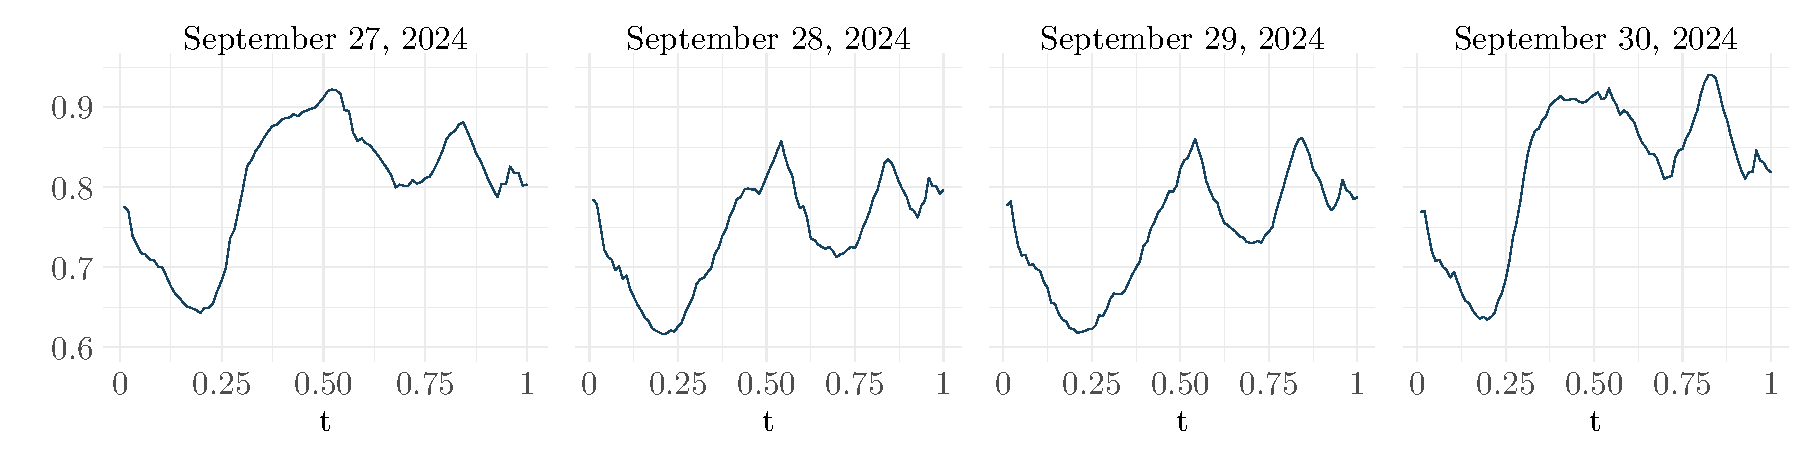
\includegraphics[width=\textwidth]{./figures/real_data_conso_4last_curves.pdf}
	\caption{\small The last four daily national electricity consumption curves in France from the dataset, with values normalised to the interval $[0,1]$.}
	\label{fig:conso_last_curves} 
\end{figure}

\begin{figure}[h!]
	\centering
	\begin{tabular}{ccc}
		\small (a) $\footnotesize \widehat{H}_t$ for simulation & \small (b) $\footnotesize \widehat{\mu}$ for simulation & \small (c) $\footnotesize \widehat{\psi}$ for simulation\\
		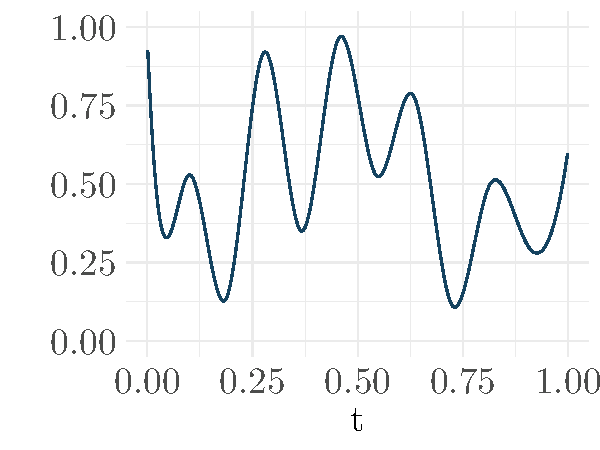
\includegraphics[width=0.3\textwidth]{./figures/local_exponent_conso.pdf} & 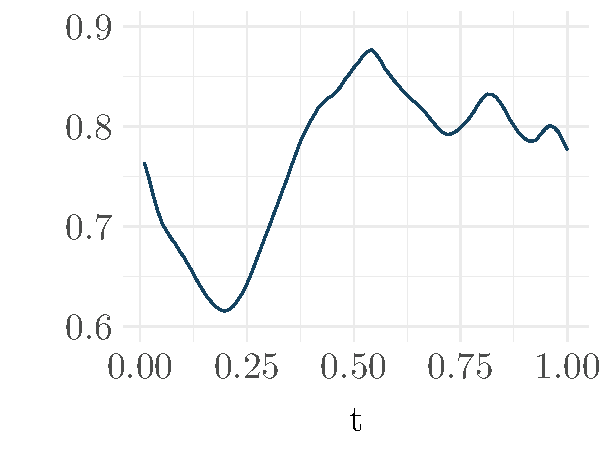
\includegraphics[width=0.3\textwidth]{./figures/smooth_mean_conso.pdf} &
		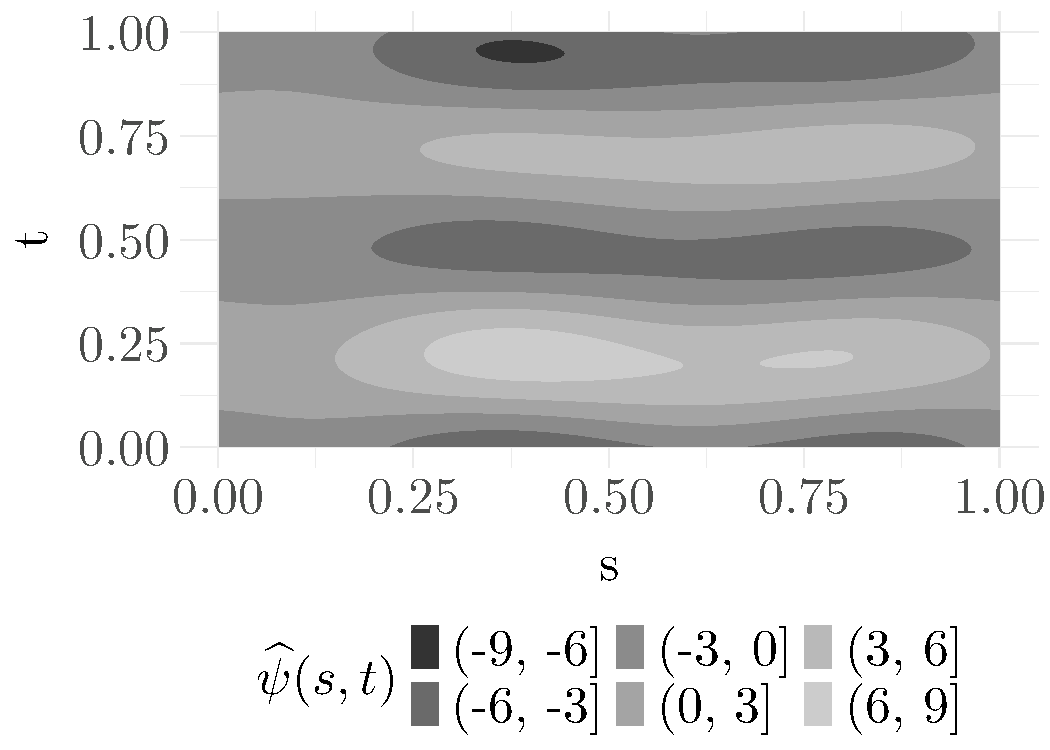
\includegraphics[width=0.3\textwidth]{./figures/far_kernel_conso.pdf}
	\end{tabular}
	\caption{\small Simulation parameters estimated from consumption curves: (a) estimated local exponent function, (b) estimated mean function, (c) estimated autoregressive kernel.}
	\label{fig:simu_param}
\end{figure}

To obtain the data points according to \eqref{eq:model}, the number of points on each curve, $M_n$, is randomly generated from a uniform distribution between $0.8\lambda$ and $1.2\lambda$, while the observation times $\{T_{n,i}\}$ are drawn independently from a uniform distribution on the interval $(0,1]$. We set $L_t = 0.1$, corresponding to the mean of the estimates of the local Hölder constant of the consumption curves, evaluated over an equidistant grid of $99$ points between $0.01$ and $0.99$, and obtained using the estimator proposed by \citet{Maissoro2025}. For the observation error term, we set $\sigma(T_{n,i}) = 0.007$, corresponding to the mean standard deviation of the consumption curves estimated using \eqref{eq:blup:sigma_estimator} over the observation grid, and the $\varepsilon_{n,i}$ are centred Gaussian variables with unit variance. A sequence of $100$ burn-in steps is used to initialise \eqref{blup:FTS_mod1}. Figure~\ref{fig:generated_last_curves} illustrates the simulated sample paths and the randomly observed points for a sample size of $(N, \lambda) = (150, 25)$.      


\begin{figure}[t!]
	\centering
	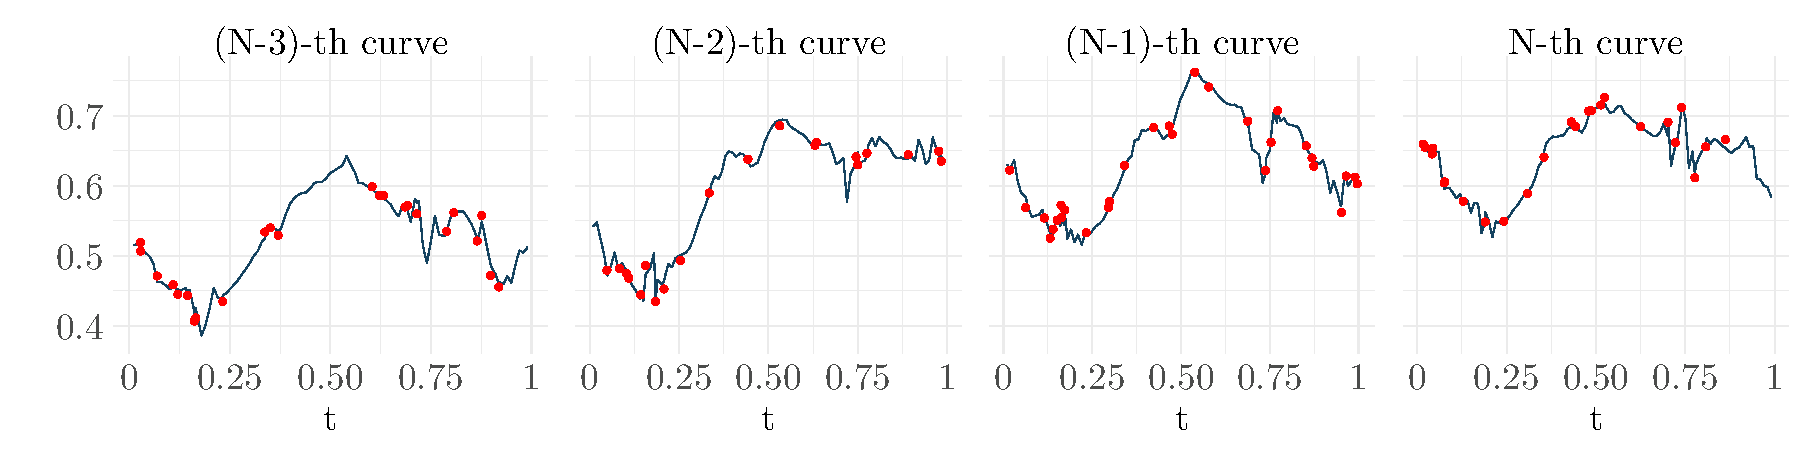
\includegraphics[width=\textwidth]{./figures/generated_conso_4last_curves.pdf}
	\caption{\small Last four simulated curves generated using the simulation setting with a sample size of $(N, \lambda) = (150, 25)$. The solid lines represent the sample paths, while the dots indicate the randomly observed noisy points on each curve, with an average of $\lambda = 25$ points per curve.}  
	\label{fig:generated_last_curves} 
\end{figure}

Finally, for the (auto)covariance study we generate different samples of FTS, whereas for the BLUP study we generate a single sample of FTS and regenerate its last curve. The aim of the (auto)covariance study is to show that the proposed method performs at least as well as the approach of \cite{Maissoro2025}, which uses a single bandwidth. Meanwhile, the aim of the BLUP study is to show that a curve, here the last curve, is accurately reconstructed.

\begin{figure}[h!]
	\centering
	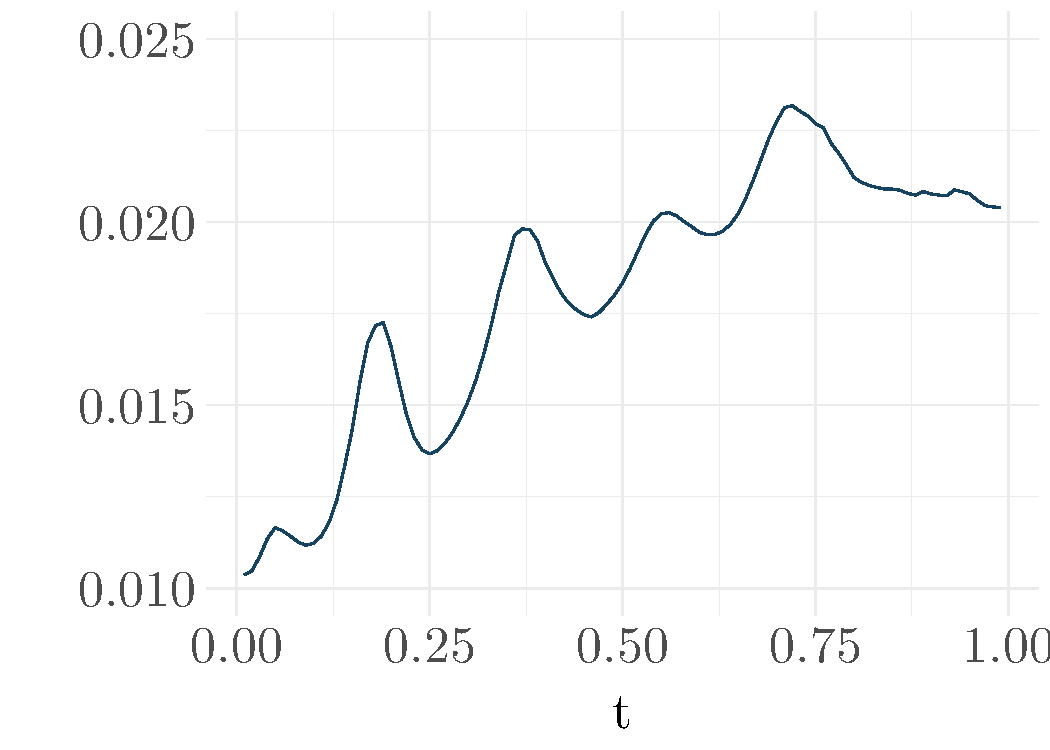
\includegraphics[width=0.4\textwidth]{./figures/variance_FTS_new_design_conso_lag=0.pdf} 
	\caption{\small Variance of the constructed FTS process from \eqref{blup:FTS_mod1} and the consumption curves.}
	\label{fig:var_FTSConso}
\end{figure}


\subsection{Implementation details}
The estimation of the lag-$\ell$, $\ell \geq 0$, (auto)covariance using the estimators in \eqref{eq:hat_Gamma_ell}, \eqref{eq:hat_Gamma_0:diagonal_outside}, and \eqref{eq:hat_Gamma_0:diagonal} involves selecting optimal bandwidths based on the data-driven rules given in \eqref{eq:gamma:risk-minimization}, \eqref{eq:gamma_0:diagonal_outside:risk-minimization}, and \eqref{eq:gamma_0_diag:risk-minimization}, respectively. Computing $\widehat{R}_{\Gamma_\ell}$ requires estimating the dependence coefficients $\mathbb{D}_\ell(s, t; h_s, h_t)$, $\mathbb{D}_\ell(t,h_t|s,h_s)$, and $\mathbb{D}(t; h_t)$, which is computationally intensive.
To reduce computation time, we adopt a simplified approach. Let $\widetilde{X}_n$ denote the NW estimator of the curve $X_n$, obtained using a bandwidth selected via cross-validation. Given a set of sample points $\{(Y_{n,1}, T_{n,1}), \ldots, (Y_{n,M_n}, T_{n,M_n})\}$ for a curve $X_n$, the cross-validated optimal bandwidth for the estimator in \eqref{eq:blup:LP_est_v} is defined as
\begin{equation}\label{eq:NW_bw_cv}
	h^* \in \argmin_h \sum_{i = 1}^{M_n}\left\{Y_{n,i} - \widetilde{X}_n^{(-i)}(T_{n,i};h)\right\}^2,
\end{equation}
where $\widetilde{X}_n^{(-i)}(T_{n,i};h)$ denotes the estimator in \eqref{eq:blup:LP_est_v} computed without the $i$-th observation and using bandwidth $h$. Moreover, let $\widetilde{Z}_n(t) = \widetilde{X}_n(t) - \widetilde{\mu}_N(t)$, and define, for all $s, t \in I$,
\begin{equation*}
	\widetilde{\mu}_N(t) = \frac{1}{N} \sum_{n=1}^{N} \widetilde{X}_{n}(t), \qquad
	\widetilde{\Gamma}_\ell(s, t) = \frac{1}{N - \ell} \sum_{n = 1}^{N - \ell} \widetilde{Z}_n(s) \widetilde{Z}_{n + \ell}(t), \quad \ell \geq 1.
\end{equation*}
Then, instead of estimating $\mathbb{D}_\ell(s, t; h_s, h_t)$, $\mathbb{D}_\ell(t,h_t|s,h_s)$, and $\mathbb{D}(t; h_t)$, we simply consider the following 
\begin{multline}
	\widehat{\mathbb{D}}_\ell(s,t;h_s, h_t) 
	= \frac{1}{N-\ell} \sum_{n=1}^{N - \ell} \left\{\widetilde{Z}_n(s) \widetilde{Z}_{n + \ell}(t) - \widetilde{\Gamma}_\ell (s,t)\right\}^2 \\
	+ \!\!\!\!\sum_{k = 1}^{N-\ell - 1}\frac{2 P_{N,\ell}^{-1}(s, t; h_s, h_t)}{N - \ell - k} \Biggl|\sum_{n = 1}^{N - \ell - k - 1}\!\left\{\widetilde{Z}_n(s) \widetilde{Z}_{n + \ell}(t) - \widetilde{\Gamma}_\ell (s,t)\right\} \left\{\widetilde{Z}_{n + k}(s) \widetilde{Z}_{n + \ell + k}(t) - \widetilde{\Gamma}_\ell (s,t)\right\}\!\Biggr|,
\end{multline}
\begin{multline}
	\widehat{\mathbb{D}}_\ell(t,h_t|s,h_s)  = 24 \!\!\!\!\!\!\!\!\!\!\!\!\!\!\!\!\!\sum_{1\leq n_1<n_2<n_3\leq \ell_{\max}}\!\!\!\!\!\!\!\!\!\!\!\!\!\!\!\!(N - n_3)^{-1}\left|\sum_{k=1}^{N - n_3} \!\! \frac{p_{k,n_1, n_2}(t;h_t)}{P_{N,\ell}^{3}(s, t; h_s, h_t)} \left\{\widetilde{Z}_k \widetilde{Z}_{k + n_1} \widetilde{Z}_{k + n_2} \widetilde{Z}_{k + n_3}\right\}(t) \right| \\
	+ 6 \!\!\!\!\!\!\!\!\!\!\!\!\!\!\sum_{1\leq n_1<n_2\leq \ell_{\max}} \!\!\!\!\!\!\!\!\!\!\!\!\!(N - n_2)^{-1}\left|\sum_{k=1}^{N - n_2} \! \frac{p_{k,n_1, n_2, n_3}(t;h_t)}{P_{N,\ell}^{3}(s, t; h_s, h_t)} \left\{\widetilde{Z}_k^2 \widetilde{Z}_{k + n_1} \widetilde{Z}_{k + n_2} + \widetilde{Z}_k \widetilde{Z}_{k + n_1}^2 \widetilde{Z}_{k + n_2} + \widetilde{Z}_k \widetilde{Z}_{k + n_1} \widetilde{Z}_{k + n_2}^2\right\}(t)\right|,
\end{multline}
\begin{multline}
	\widehat{\mathbb{D}}(t; h_t)  = 24 \!\!\!\!\!\!\!\!\!\!\!\!\!\!\!\!\!\sum_{1\leq n_1<n_2<n_3\leq \ell_{\max}}\!\!\!\!\!\!\!\!\!\!\!\!\!\!\!\!(N - n_3)^{-1}\left|\sum_{k=1}^{N - n_3} \!\! \frac{p_{k,n_1, n_2}(t;h_t)}{P_N^{3}(t; h_t)}\left\{\widetilde{Z}_k \widetilde{Z}_{k + n_1} \widetilde{Z}_{k + n_2} \widetilde{Z}_{k + n_3}\right\}(t) \right| \\ 
	+ 6 \!\!\!\!\!\!\!\!\!\!\!\!\!\!\sum_{1\leq n_1<n_2\leq \ell_{\max}} \!\!\!\!\!\!\!\!\!\!\!\!\!(N - n_2)^{-1}\left|\sum_{k=1}^{N - n_2} \!\frac{p_{k,n_1, n_2, n_3}(t;h_t)}{P_N^{3}(t; h_t)} \left\{\widetilde{Z}_k^2 \widetilde{Z}_{k + n_1} \widetilde{Z}_{k + n_2} + \widetilde{Z}_k \widetilde{Z}_{k + n_1}^2 \widetilde{Z}_{k + n_2} + \widetilde{Z}_k \widetilde{Z}_{k + n_1} \widetilde{Z}_{k + n_2}^2\right\}(t)\right|,
\end{multline}
where $N \gg \ell_{\max} = 3$ to avoid $\Oo(N^4)$ or $\Oo(N^3)$ complexity, and 
\begin{align}
	p_{k,n_1, n_2}(t;h_t) &= \pi_k(t;h_t)\pi_{k+n_1}(t;h_t)\pi_{k+n_2}(t;h_t), \\
	p_{k,n_1, n_2, n_3}(t;h_t) &= \pi_k(t;h_t)\pi_{k+n_1}(t;h_t)\pi_{k+n_2}(t;h_t)\pi_{k+n_3}(t;h_t).
\end{align}

\subsection{Autocovariance function estimation}\label{sec:emp_study:autocov}
We consider the pairs $(N, \lambda) \in \{150, 300, 600\} \times \{25, 50, 100, 200\}$ and generate $R = 400$ independent FTS. For each sample, the aim is to estimate the autocovariance using both the single-bandwidth estimator proposed by \cite{Maissoro2025} and our new estimator, which uses two bandwidth parameters. Hereafter, we refer to the estimator of \cite{Maissoro2025} as \texttt{MPV24}. The adaptive estimation of the autocovariance function via the estimator given in \eqref{eq:hat_Gamma_ell} involves selecting optimal bandwidths by minimising the risk function defined in \eqref{eq:risk-Gamma}. First, we consider the estimation of this risk function and then present a performance comparison with \color{magenta}the \texttt{MPV24} estimator\color{black}.

To this end, we consider four pairs $(s, t)$ and compute the average of the lag-$1$ autocovariance risk function $\widehat{R}_{\Gamma_1}(s, t; h_s, h_t)$, as defined in \eqref{eq:risk-Gamma}, over a bandwidth grid $\Hh_N \times \Hh_N$ based on the $R = 400$ FTS replications. Figure~\ref{fig:autocov_risk_2bw} shows the mean of the $400$ replications of the estimates of the lag-$1$ autocovariance risk function for $(N, \lambda) = (150, 100)$ at four locations $(s,t)$. The estimates of the risk function are a convex function of $(h_s, h_t)$ for all pairs $(s,t)$. Furthermore, since the regularity varies along the domain (see Figure~\ref{fig:simu_param}-(a)), as expected, the minima bandwidth pairs $(h_1^*(s|t), h_1^*(t|s))$ are reached such that $h_1^*(s|t) \neq h_1^*(t|s)$, when $H_s \neq H_t$. Moreover, the difference between the selected bandwidths is greater for pairs $(s,t)$ such that $|H_s-H_t|$ is large. 
%For instance, at $(s,t) = (0.2, 0.8)$, the optimal bandwidths are $(h_1^*(s|t), h_1^*(t|s)) = (0.022, 0.010)$, reflecting the regularity $(H_s, H_t) \approx (0.4, 0.8)$. In contrast, at $(s,t) = (0.7, 0.8)$, where the regularity is approximately $(H_s, H_t) \approx (0.8, 0.8)$, the optimal bandwidths are identical, $(h_1^*(s|t), h_1^*(t|s)) = (0.022, 0.022)$.
\begin{figure}[h!]
	\centering
	\begin{tabular}{cc}
		$(s, t)= (0.2, 0.3)$ & $(s, t)= (0.5, 0.2)$\\
		$(H_s, H_t)= (0.199, 0.844)$ & $(H_s, H_t)= (0.784, 0.199)$\\
		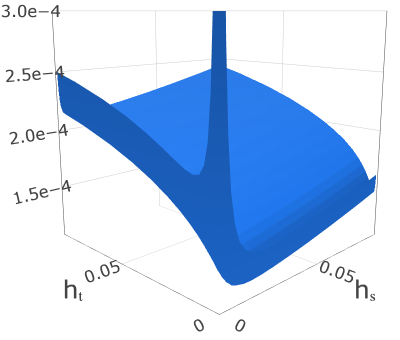
\includegraphics[width=0.35\textwidth]{./figures/autocov/plt_autocov_risk_conso_new_design_N=150_lambda=100_s=0.2_t=0.3.png} & 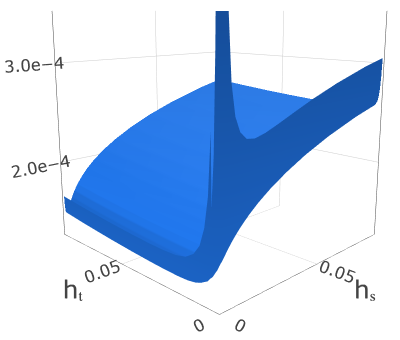
\includegraphics[width=0.35\textwidth]{./figures/autocov/plt_autocov_risk_conso_new_design_N=150_lambda=100_s=0.5_t=0.2.png}\\
		$(h_1^*(s|t), h_1^*(t|s)) = (0.001, 0.016)$ & $ (h_1^*(s|t), h_1^*(t|s)) = (0.021, 0.001)$ \\
		& \\
		& \\
		$(s, t)= (0.1, 0.4)$ & $(s, t)= (0.8, 0.5)$\\
		$(H_s, H_t)= (0.529, 0.527)$ & $(H_s, H_t)= (0.445, 0.784)$\\
		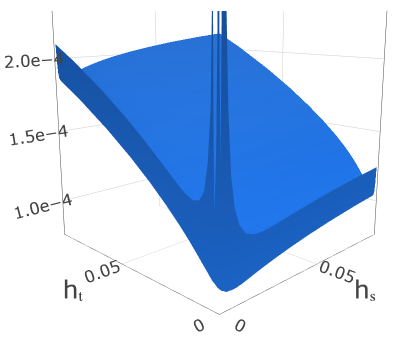
\includegraphics[width=0.35\textwidth]{./figures/autocov/plt_autocov_risk_conso_new_design_N=150_lambda=100_s=0.1_t=0.4.png} &
		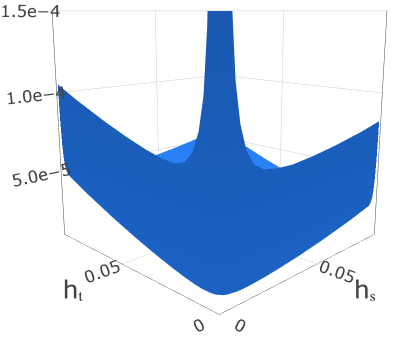
\includegraphics[width=0.35\textwidth]{./figures/autocov/plt_autocov_risk_conso_new_design_N=150_lambda=100_s=0.8_t=0.5.png}\\
		$(h_1^*(s|t), h_1^*(t|s)) = (0.003, 0.007)$ & $(h_1^*(s|t), h_1^*(t|s)) = (0.009, 0.012)$ 
	\end{tabular}
	\caption{\small Empirical average of the risk function $\widehat{R}_{\Gamma_1}(s,t;h_s, h_t)$ at $(s,t) \in \{ (0.2, 0.3)$, $(0.5, 0.2)$, $(0.1, 0.4)$, $(0.8, 0.5)\}$ computed over $400$ independent replications of the FTS for the sample size $(N, \lambda) = (150, 100)$. For each $(s,t)$, the optimal bandwidths $(h_1^*(s|t), h_1^*(t|s))$ corresponding to the plotted risk function are indicated at the bottom of the respective panel.}
	\label{fig:autocov_risk_2bw}
\end{figure}

We conclude this section with a performance comparison of the new autocovariance estimator against the \texttt{MPV24} estimator, which uses a single bandwidth. Let $\widehat{\Gamma}_{N,\ell}^{(i)}$ denote our new estimator computed from the $i$-th replication ($i = 1, \ldots, R = 400$), and let $\widehat{\Gamma}_{\texttt{MPV24}, \ell}^{(i)}$ denote the corresponding \texttt{MPV24} estimator. For benchmarking, we use the empirical infeasible estimator, denoted by ${\widehat{\Gamma}}_{N', \ell}$, which is computed on a large sample of size $N'$. This estimator is feasible in simulation settings. That is,
\begin{equation}
	\widehat{\Gamma}_{N', \ell}(s, t) = \frac{1}{N' - \ell} \sum_{n=1}^{N' - \ell} \left\{X_{n}(s) - \widehat{\mu}_{N'}(s)\right\} \left\{X_{n+\ell}(t) - \widehat{\mu}_{N'}(t)\right\},
	\qquad \text{where} \quad
	\widehat{\mu}_{N'}(t) = \frac{1}{N'} \sum_{n=1}^{N'} X_n(t).
\end{equation}
Then, for each $i = 1, \ldots, R$, we compute the pointwise error ratio:
\begin{equation}\label{eq:error_ratio_autocov}
	\forall (s, t) \in I^2, \quad
	E_\ell^{(i)}(s, t) = \frac{\left| \widehat{\Gamma}_{N,\ell}^{(i)}(s, t; h_\ell^*(s|t), h_\ell^*(t|s)) - \widehat{\Gamma}_{N',\ell}(s, t) \right|}{\left| \widehat{\Gamma}_{\texttt{MPV24}, \ell}^{(i)}(s, t; h^*) - \widehat{\Gamma}_{N',\ell}(s, t) \right|}.
\end{equation}
With $N' = 5000$, we compute the error ratios $\{E_1^{(i)}(s, t),\; i = 1, \ldots, R\}$ for the lag-1 autocovariance estimator at four locations $(s, t)$. Figure~\ref{fig:autocov_ratio_FTS_Conso} presents the corresponding boxplots across all $(N, \lambda)$ configurations. As anticipated from Theorem~\ref{thm:Gamma}, the new estimator significantly outperforms \texttt{MPV24} when the local regularities $H_s$ and $H_t$ differ, with greater gains observed for pairs $(s, t)$ such that $|H_s - H_t|$ is large. For instance, the largest improvements are found at $(s, t) = (0.2, 0.3)$ and $(0.5, 0.2)$, where $(H_{0.2}, H_{0.3}) = (0.199, 0.844)$ and $(H_{0.5}, H_{0.2}) = (0.784, 0.199)$, respectively. In contrast, at $(s, t) = (0.8, 0.5)$, where $(H_{0.8}, H_{0.5}) = (0.445, 0.784)$, the two estimators tend to perform similarly as the sample size increases.

\begin{figure}[h!]
	\centering
	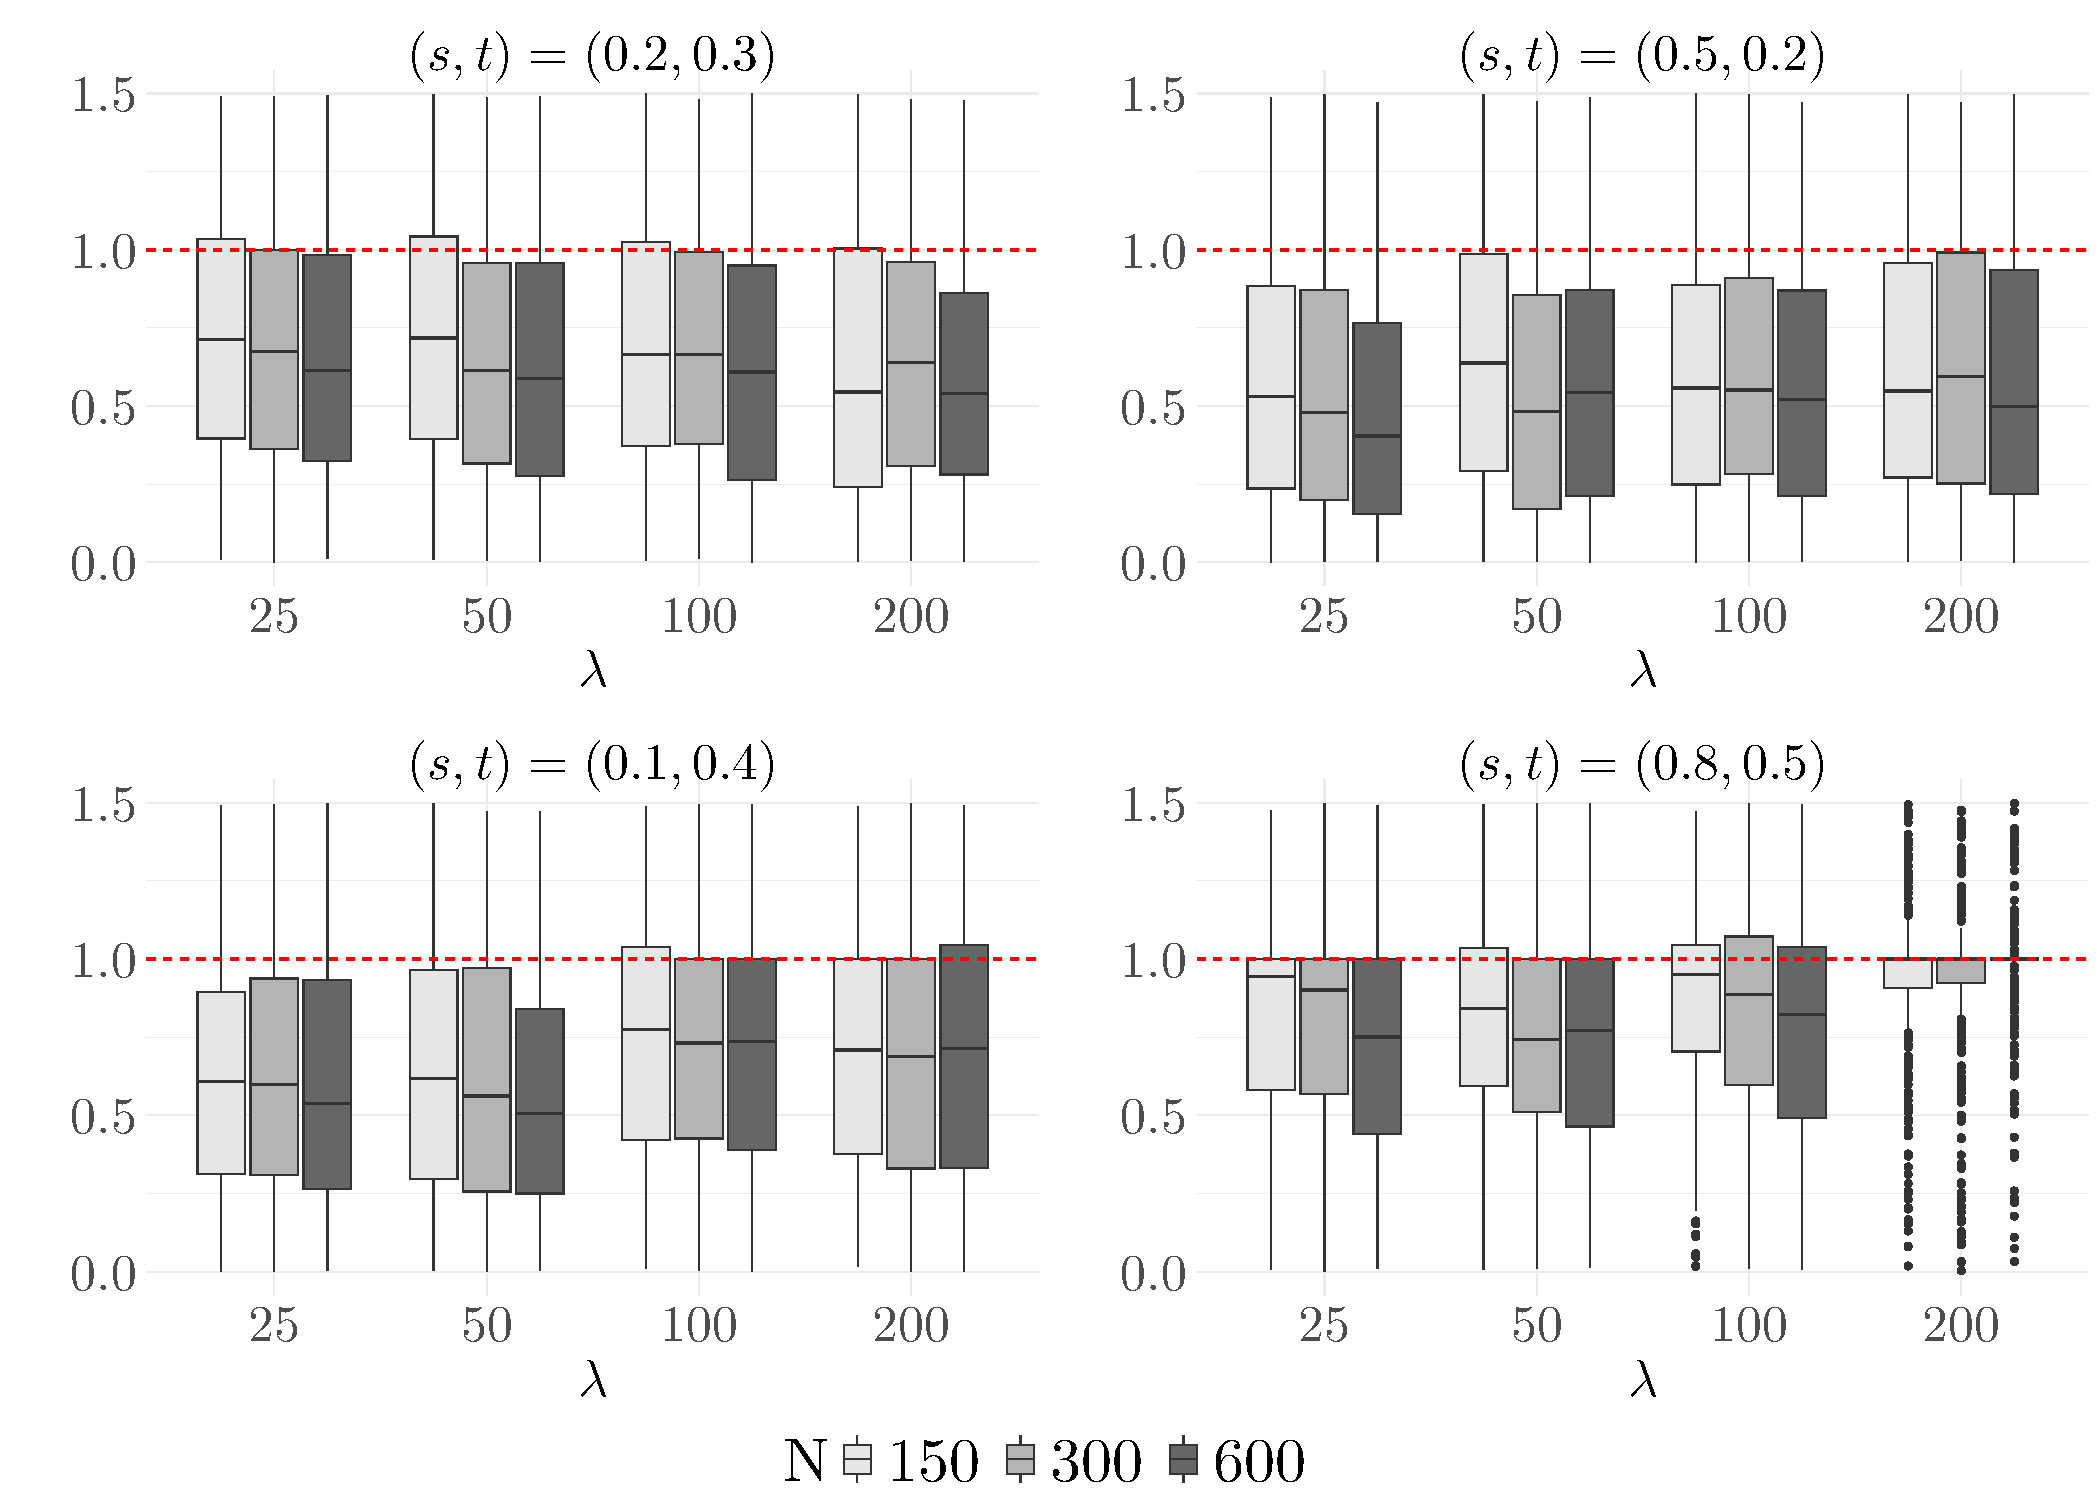
\includegraphics[width=0.9\textwidth]{./figures/autocov/boxplot_conso_autocov_ratio_new_design_lag=1_all_bis.pdf}
	\caption{\small Boxplots of the error ratio \eqref{eq:error_ratio_autocov} of the lag-1 autocovariance estimator for four pairs $(s, t) \in \{(0.2, 0.3)$, $(0.5, 0.2)$, $(0.1, 0.4)$, $(0.8, 0.5)\}$. For each pair, the corresponding values of the local exponent function are $(H_{0.2}, H_{0.3}) = (0.199, 0.844)$, $(H_{0.5}, H_{0.2}) = (0.784, 0.199)$, $(H_{0.1}, H_{0.4}) = (0.529, 0.527)$, and $(H_{0.8}, H_{0.5}) = (0.445, 0.784)$.}
	\label{fig:autocov_ratio_FTS_Conso}
\end{figure}

\subsection{Covariance function estimation}\label{sec:emp_study:cov}
Our new adaptive covariance estimator involves selecting optimal bandwidths by minimising both the estimates of the bivariate risk function \eqref{eq:risk-Gamma_0:diagonal_outside} outside the diagonal band and the estimates of the univariate risk function given in \eqref{eq:risk-Gamma_0} for the diagonal line estimator. We consider the same scenario and generated data as in the autocovariance estimation study to illustrate the performance of our new covariance estimator.  

First, regarding the risk function estimation, Figure~\ref{fig:cov_risk_2bw} shows the average over the $400$ replications of the estimates of the covariance risk function \eqref{eq:risk-Gamma_0:diagonal_outside} for $(N, \lambda) = (150, 100)$ at four locations. These plots provide evidence that the risk function is convex and can thus be effectively minimised to obtain optimal bandwidth pairs. Similarly, Figure~\ref{fig:diagonal_risk} illustrates that the risk function for the diagonal line is also convex, allowing straightforward selection of the optimal bandwidth for its estimation.

Furthermore, for the bivariate risk function \eqref{eq:risk-Gamma_0:diagonal_outside}, since the regularity varies across the domain (see Figure~\ref{fig:simu_param}-(a)), the optimal bandwidth pairs $(h_0^*(s|t), h_0^*(t|s))$ are typically such that $h_0^*(s|t) \neq h_0^*(t|s)$ when $H_s \neq H_t$. The difference between the selected bandwidths becomes more pronounced for pairs $(s, t)$ with large differences in local regularity, that is, when $|H_s - H_t|$ is large.

\begin{figure}[h!]
		\centering
	\begin{tabular}{cc}
		$(s, t)= (0.2, 0.3)$ & $(s, t)= (0.5, 0.2)$\\
		$(H_s, H_t)= (0.199, 0.844)$ & $(H_s, H_t)= (0.784, 0.199)$\\
		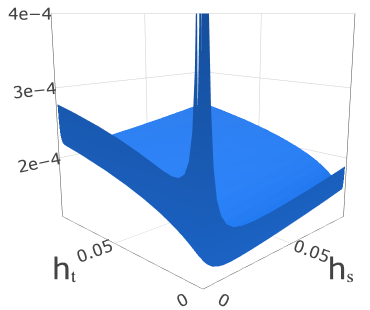
\includegraphics[width=0.35\textwidth]{./figures/cov/plt_cov_risk_conso_new_design_N=150_lambda=100_s=0.2_t=0.3.png} & 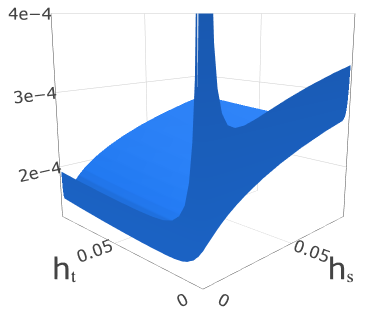
\includegraphics[width=0.35\textwidth]{./figures/cov/plt_cov_risk_conso_new_design_N=150_lambda=100_s=0.5_t=0.2.png}\\
		$(h_0^*(s|t), h_0^*(t|s)) = ( 0.002, 0.016)$ & $ (h_0^*(s|t), h_0^*(t|s)) = (0.021, 0.002)$ \\
		& \\
		& \\
		$(s, t)= (0.1, 0.4)$ & $(s, t)= (0.8, 0.5)$\\
		$(H_s, H_t)= (0.529, 0.527)$ & $(H_s, H_t)= (0.445, 0.784)$\\
		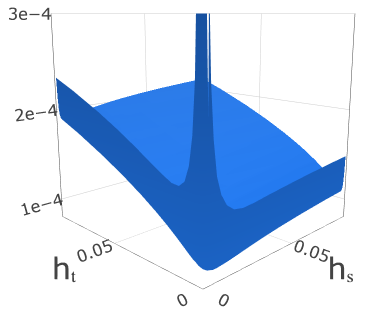
\includegraphics[width=0.35\textwidth]{./figures/cov/plt_cov_risk_conso_new_design_N=150_lambda=100_s=0.1_t=0.4.png} &
		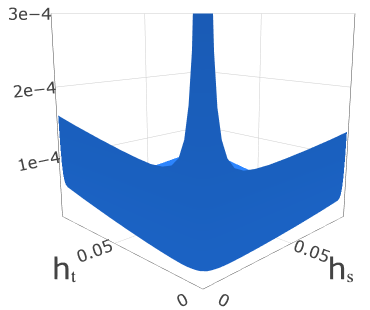
\includegraphics[width=0.35\textwidth]{./figures/cov/plt_cov_risk_conso_new_design_N=150_lambda=100_s=0.8_t=0.5.png}\\
		$(h_0^*(s|t), h_0^*(t|s)) = (0.003, 0.007)$ & $(h_0^*(s|t), h_0^*(t|s)) = (0.009, 0.016)$
	\end{tabular}
	\caption{\small Empirical average of the risk function $\widehat{R}_{\Gamma_0}(s,t;h_s, h_t)$ at $(s,t) \in \{ (0.2, 0.3)$, $(0.5, 0.2)$, $(0.1, 0.4)$, $(0.8, 0.5)\}$ computed over $400$ independent replications of the FTS for the sample size $(N, \lambda) = (150, 100)$. For each $(s,t)$, the optimal bandwidths $(h_0^*(s|t), h_0^*(t|s))$ corresponding to the plotted risk function are indicated at the bottom of the respective panel.}
	\label{fig:cov_risk_2bw}
\end{figure}
\begin{figure}[th]
	\vspace{.1cm}
	\centering
	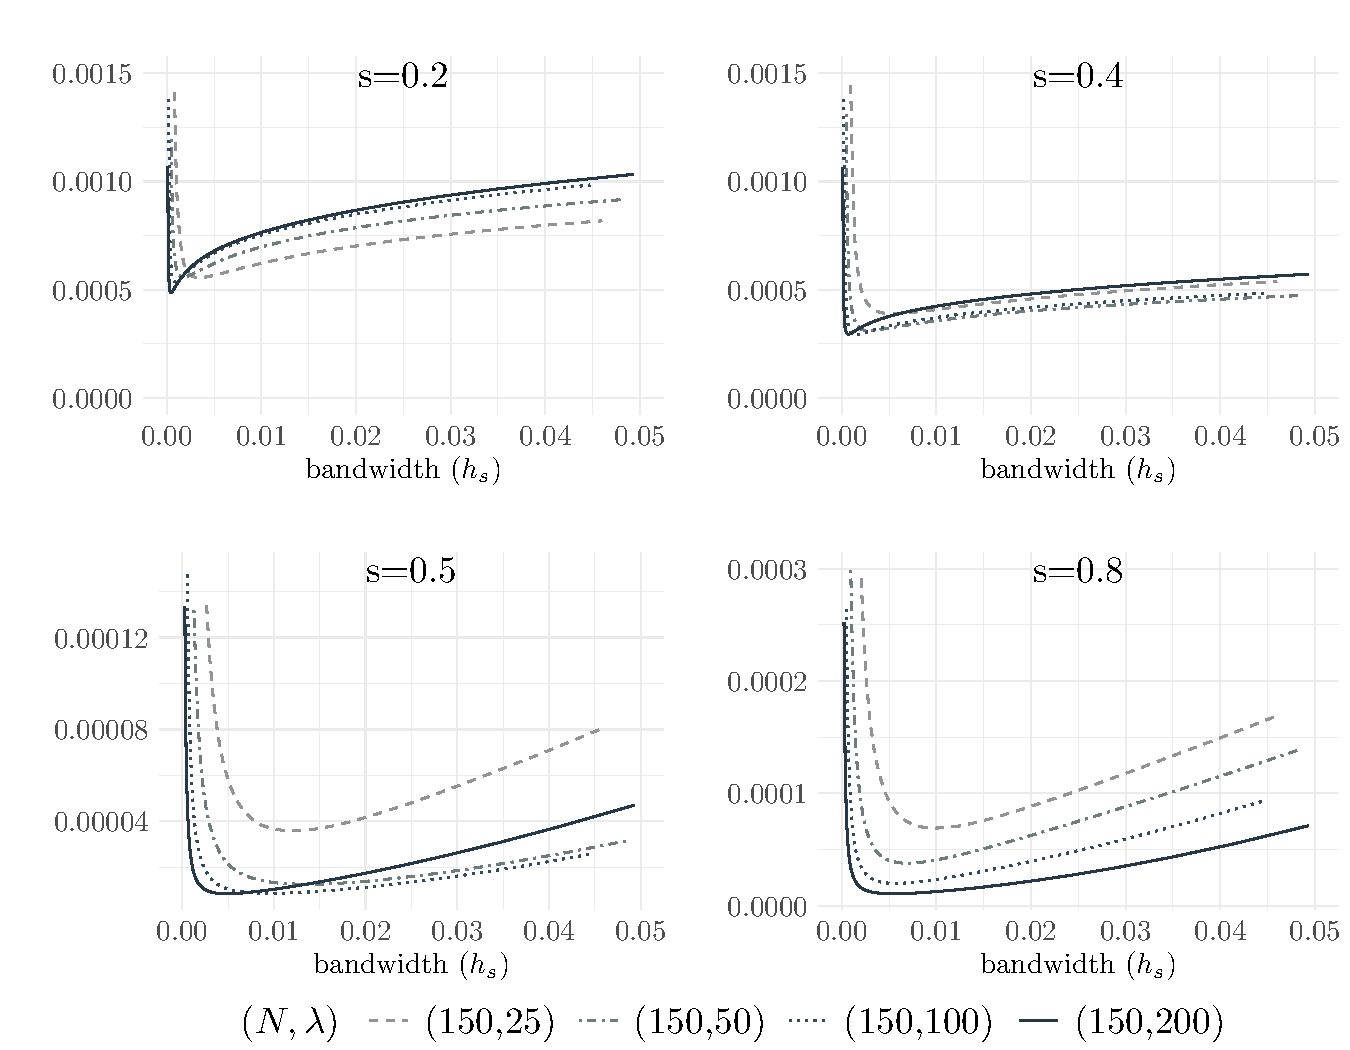
\includegraphics[width=0.9\linewidth]{./figures/cov/plt_diag_cov_risk_conso_new_design_N=150_all_lambda_all_s.pdf}
	\caption{\small Empirical average of the risk function $\widehat{R}_\mu(s, h_s)$ at $s \in \{0.2, 0.4, 0.5, 0.8\}$, computed over $400$ independent replications of the FTS for sample sizes $(N, \lambda) \in \{(150, 25), (150, 50), (150, 100), (150, 200)\}$.}
	\label{fig:diagonal_risk}
\end{figure}

We conclude this section with a performance comparison between our proposed covariance estimator and its version that selects the same bandwidth for both arguments of the function. The error in \eqref{eq:error_ratio_autocov} is then computed with respect to that covariance estimator instead of to the \texttt{MPV24} estimator. For simplicity, we do not restate the formula. Figure~\ref{fig:cov_ratio_FTS_Conso} shows boxplots of the error ratio of the covariance estimator for four $(s, t)$ pairs across different sample size configurations $(N, \lambda)$. As anticipated from Theorem~\ref{thm:Gamma_0}, our estimator significantly outperforms the covariance estimator that uses the same local optimal bandwidth for both arguments, when the local regularities $H_s$ and $H_t$ differ, and the gain increases with larger values of $|H_s - H_t|$.

\begin{figure}[h!]
	\centering
	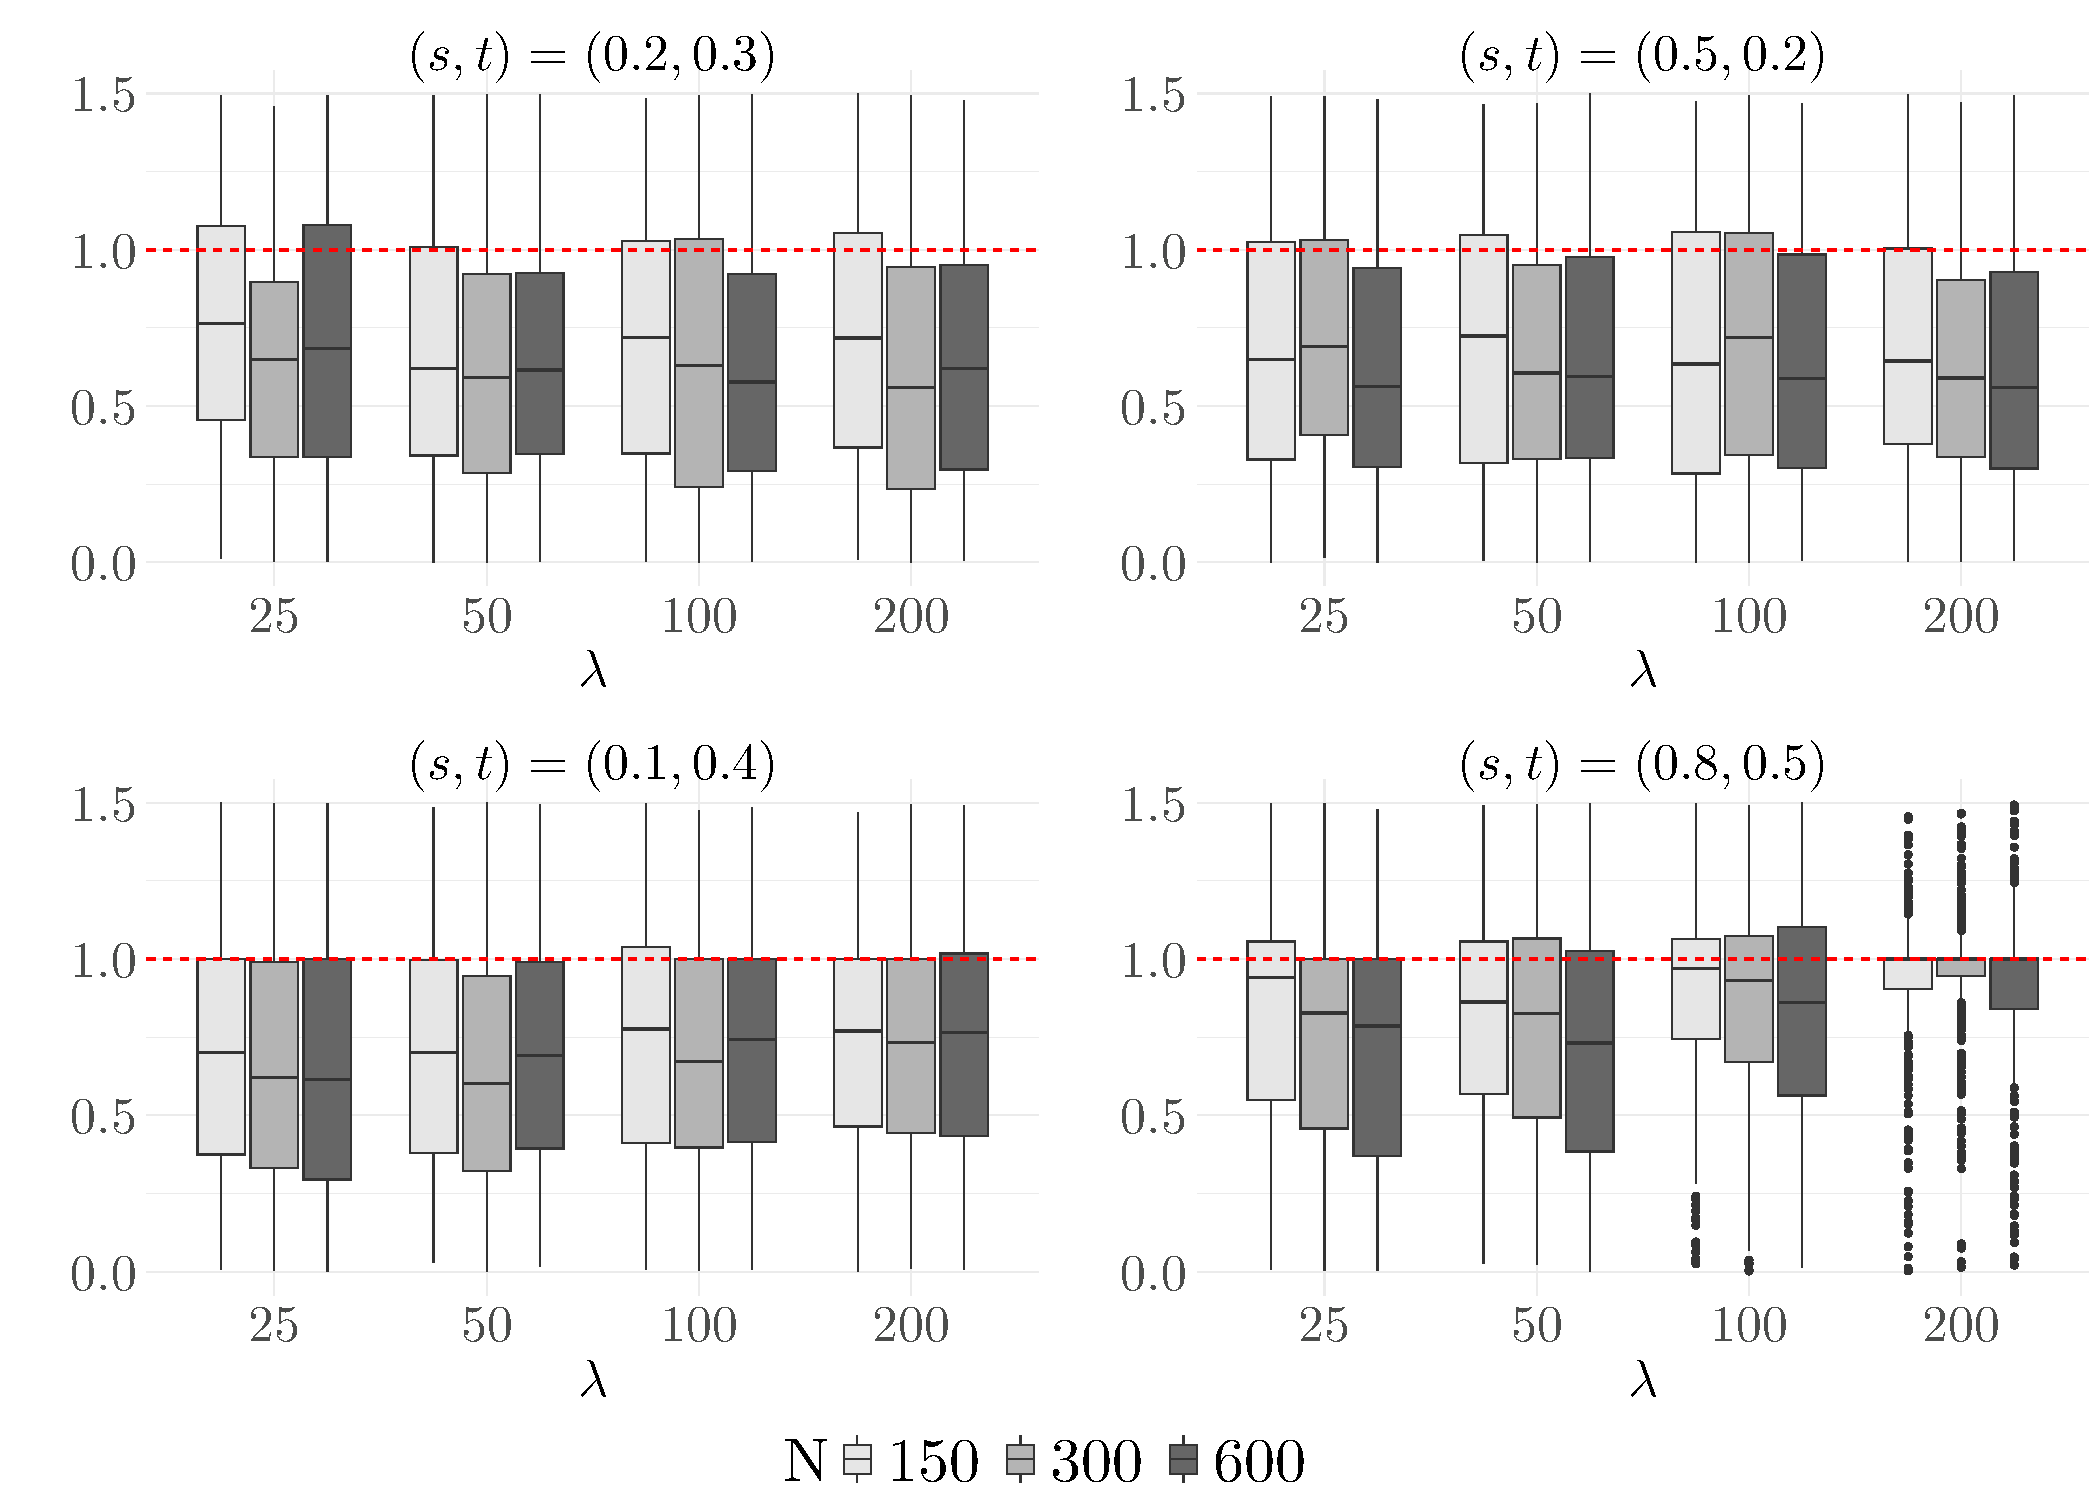
\includegraphics[width=0.9\textwidth]{./figures/cov/boxplot_conso_cov_ratio_new_desing_lag=0_all_bis.pdf}
	\caption{\small Boxplot of the error ratio \eqref{eq:error_ratio_autocov} of the covariance estimator for four pairs $(s, t) \in \{(0.2, 0.3)$, $(0.5, 0.2)$, $(0.1, 0.4)$, $(0.8, 0.5)\}$. For each pair, the corresponding values of the local exponent function are $(H_{0.2}, H_{0.3}) = (0.199, 0.844)$, $(H_{0.5}, H_{0.2}) = (0.784, 0.199)$, $(H_{0.1}, H_{0.4}) = (0.529, 0.527)$, and $(H_{0.8}, H_{0.5}) = (0.445, 0.784)$.} 
	\label{fig:cov_ratio_FTS_Conso}
\end{figure}

\subsection{Adaptive curve prediction}
In this section, we study the performance of the adaptive BLUP through Monte Carlo simulations. Since the adaptive BLUP leverages information from both the current curve and the lagged curve, we first examine the empirical autoregressive effect and then present the Monte Carlo results.

\subsubsection{Empirical autoregressive effect}

Recall that the adaptive BLUP depends on adaptive estimates of the mean, covariance, and lag-$1$ autocovariance functions. To describe the strength of dependence between the current and lagged curves, we compute a functional analogue of the autocorrelation function for real-valued time series. The Functional Autocorrelation Function (FACF) at lag~$\ell$, considered by \citet{horovath_2016}, is defined as
\begin{equation}\label{eq:blup:facf}
	\widehat{\rho}_\ell = 
	\|\widehat{\Gamma}_{N,\ell}\|\left[\int \widehat{\Gamma}_{N,0}(t,t)dt\right]^{-1},
\end{equation}
where $\widehat{\Gamma}_{N,\ell}$ estimates $\Gamma_\ell$, and $\|\cdot\|$ denotes the standard norm in $\mathbb{L}^2_\mathcal{H}$. Moreover, $0 \leq \widehat{\rho}_\ell \leq 1$. The FACF also serves as an empirical check for the presence of an autoregressive effect in the FTS. In fact, if there were no autoregressive effect, the FACF would equal zero, implying that the autocovariance-related top-right and bottom-left blocks in the matrix $\VV_{n_0}$ would be nil and thus contribute nothing to the adaptive BLUP.

\begin{figure}[h]
	\centering
	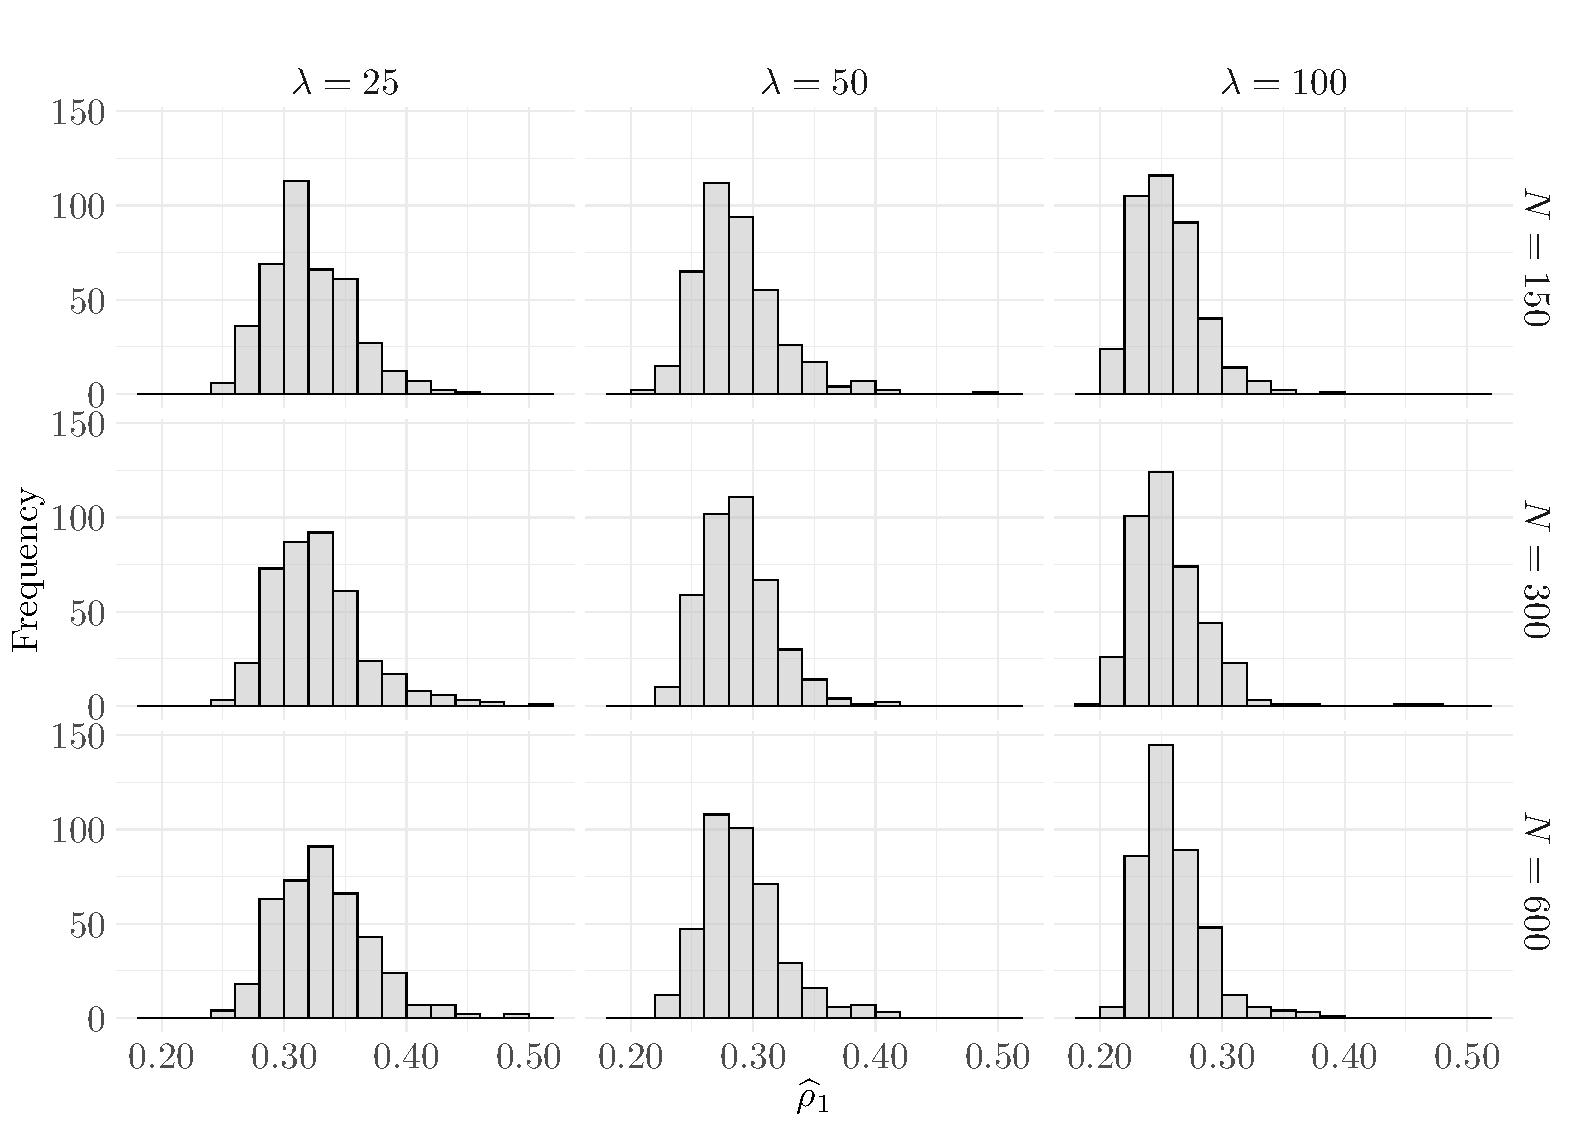
\includegraphics[width=\textwidth]{./figures/blup/hist_lag-1_facf_conso.pdf}
	\caption{\small Histograms of estimated lag-$1$ FACF values for different $(N, \lambda)$ configurations.}
	\label{fig:conso_lag1_facf}
\end{figure}

We use the same generated sample of FTS as in the study of the autocovariance function, estimate the lag-$1$ FACF for each of the $400$ FTS replications using \eqref{eq:blup:facf}, and display the resulting histograms in Figure~\ref{fig:conso_lag1_facf} for different sample sizes $(N, \lambda)$. The plots provide empirical evidence that the autocovariance-related blocks in $\VV_{n_0}$ are not nil. Moreover, for our simulated FAR(1) model, most of the lag-$1$ FACF values are concentrated between $0.2$ and $0.4$.

\subsubsection{Monte Carlo study}

We now turn to the study of the predictive performance of the adaptive BLUP through Monte Carlo simulations. Given a sample of FTS, the objective is to assess the prediction performance of its final curve, that is, $n_0 = N$, under various scenarios depending on the available observation points for that curve. To this end, we adopt a simulation setup that differs slightly from the one used in the study of the (auto)covariance function. 
We consider the pairs $(N, \lambda) \in \{150, 300, 600\} \times \{25, 50, 100\}$, generate a single sample of FTS, and regenerate its final curve $R = 400$ times.
The prediction accuracy of each regenerated final curve is then evaluated, given all or only a subset of its observed points, while maintaining the other curves of the FTS sample unchanged.

Table~\ref{tab:blup_fts_conso} shows the bias and standard deviation of the estimates of $\widehat{\mathfrak{X}}_{n_0}(t)$ obtained for the prediction of the last curve, when all observation points $\{(Y_{n_0, i}, T_{n_0,i}),\; 1\leq i \leq M_{n_0}\}$ are available. As expected, both the bias and the variance of the adaptive BLUP decrease as the sample size increases. Notably, the estimated standard deviation tends to increase with $t$. This is partly due to the sample paths becoming rougher towards the right end of the domain $I$, as illustrated by the shape of the local exponent function in Figure~\ref{fig:simu_param}-(a). Moreover, larger values of $t$ are associated with higher marginal variance $\operatorname{Var}(X_t)$, as shown in Figure~\ref{fig:var_FTSConso}. These factors lead to less accurate estimates of the mean and (auto)covariance functions, and consequently to less accurate predictions by the adaptive BLUP.

\begin{table}[!tbp]
	\begin{center}
		{\small 	
			\begin{tabular}{cccccccccccccc}
				\hline
				&&&\multicolumn{2}{c}{\bfseries $t = 0.2$}&&\multicolumn{2}{c}{\bfseries $t = 0.4$}&&\multicolumn{2}{c}{\bfseries $t = 0.7$}&&\multicolumn{2}{c}{\bfseries $t = 0.8$}\\
				\cline{4-5} \cline{7-8} \cline{10-11} \cline{13-14}
				\multicolumn{1}{c}{$N$}&\multicolumn{1}{c}{$\lambda$}&&\multicolumn{1}{c}{Bias}&\multicolumn{1}{c}{Sd}&&\multicolumn{1}{c}{Bias}&\multicolumn{1}{c}{Sd}&&\multicolumn{1}{c}{Bias}&\multicolumn{1}{c}{Sd}&&\multicolumn{1}{c}{Bias}&\multicolumn{1}{c}{Sd}\tabularnewline
				\hline
				$150$&$ 25$&&0.0229&0.1173&&-0.0187&0.1209&&0.0331&0.1404&&0.0001&0.1275\\
				$150$&$ 50$&&0.0430&0.1033&&0.1017&0.1293&&-0.0050&0.1194&&-0.0093&0.1285\\
				$150$&$100$&&-0.0085&0.1006&&0.0672&0.0994&&0.0232&0.1326&&-0.0207&0.1005\\
%				$300$&$ 25$&&0.0076&0.0885&&-0.0272&0.1052&&-0.0367&0.1036&&0.0078&0.1315\\
%				$300$&$ 50$&&0.0247&0.1392&&0.0482&0.1316&&0.0305&0.1376&&-0.0505&0.1403\\
%				$300$&$100$&&0.0192&0.1018&&0.0076&0.1291&&0.0235&0.1223&&-0.0638&0.1221\\
%				$600$&$ 25$&&0.0097&0.0932&&0.0044&0.1114&&-0.014&0.1418&&0.0019&0.1292\\
%				$600$&$ 50$&&-0.0030&0.1047&&0.0656&0.1055&&0.0457&0.1344&&-0.0243&0.1245\\
%				$600$&$100$&&-0.0437&0.1052&&0.0102&0.1222&&0.0190&0.1408&&0.0773&0.1238\\
				\hline
		\end{tabular} }
		\caption{\small Bias and standard deviation (SD) of adaptive BLUP estimates for the last curve, based on $400$ independent replications.}
		\label{tab:blup_fts_conso}
	\end{center}
\end{table}

We now compare our prediction procedure to that of \citet{rubin2020sparsely}, referred to as \texttt{RP20}, as well as to the Nadaraya–Watson (NW) estimator using a cross-validated bandwidth as defined in \eqref{eq:NW_bw_cv}. The comparison with the NW estimator is limited to the scenario where all observation points on the last curve are available. For the comparison with \texttt{RP20}, we also consider three additional scenarios in which the available observation points for the last curve lie within the subdomains $(0, 1/4]$, $(0, 1/2]$, and $(0, 3/4]$.

\begin{figure}[ht!]
	\centering
	\begin{tabular}{c}
		ISE ratio w.r.t. \texttt{NW} estimator\\
		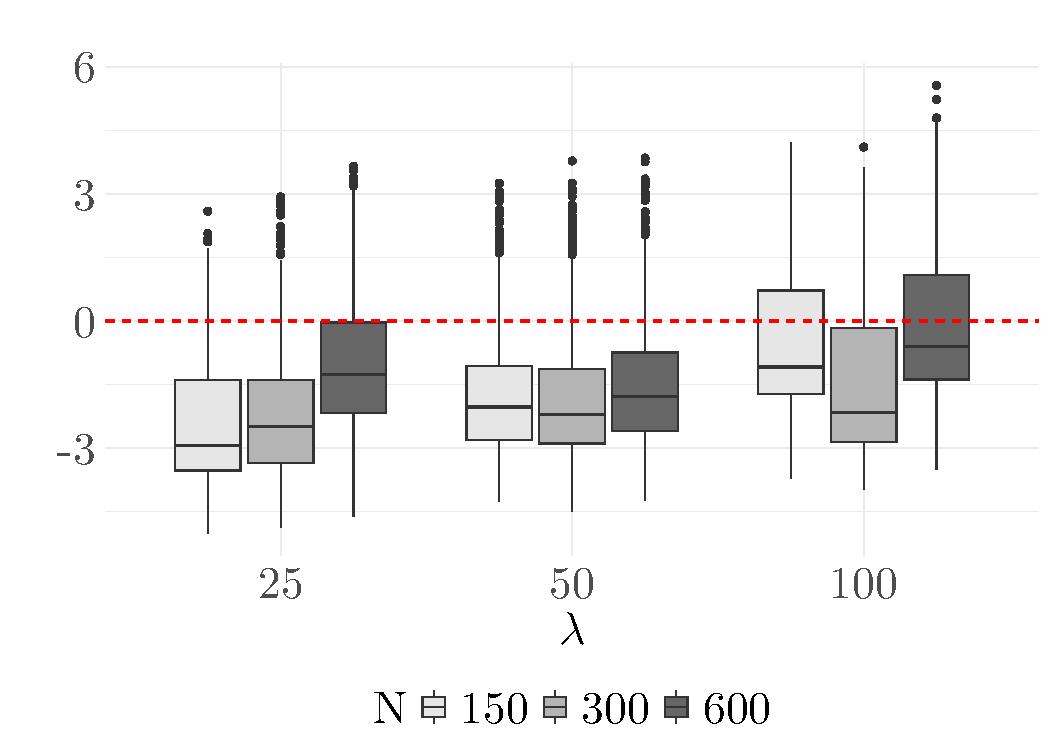
\includegraphics[width=0.5\textwidth]{./figures/blup/plot_log_ise_ratio_blup_2bw_over_nw.pdf}
	\end{tabular}
	\caption{\small Boxplots of the $\log$ ISE ratios of the adaptive BLUP relative to the NW estimator, in the scenario where all observation points of the last curve to be predicted are available.}
	\label{fig:ise_ratio_blup_nw}
\end{figure}

Let us denote by
\begin{equation}
	\mathcal{T}_{n_0}^\alpha = \{ (Y_{n,i}, T_{n, i}) \; : \; T_{N, i} \in (0, \alpha], \; 1 \leq i \leq M_{n}, \; 1 \leq n \leq N\}, \qquad \alpha=1/4, 1/2, 3/4,
\end{equation}
the set of all available observation points in the FTS, with the last curve observed only over $(0, \alpha]$. Predictions based on the data $\mathcal{T}_{n_0}^\alpha$ are compared using the ratio of integrated squared errors (ISE). Let the superscript $(k)$ denote the $k$-th replication of the last curve. Then, the ISE ratio of the adaptive BLUP relative to a given method $\texttt{Meth}$ (either NW or \texttt{RP20}) is defined as
\begin{equation}
	\text{Ratio}^{(k)}(\texttt{Meth}) = \dfrac{\int_0^1 \left(\widehat{\mathfrak{X}}_{n_0}^{(k)}(t) - X_{n_0}^{(k)}(t)\right)^2 dt}{ \int_0^1 \left(\widehat{\mathfrak{X}}_{\texttt{Meth}}^{(k)}(t) - X_{n_0}^{(k)}(t)\right)^2 dt}.
\end{equation}

\begin{figure}[h!]
	\centering
	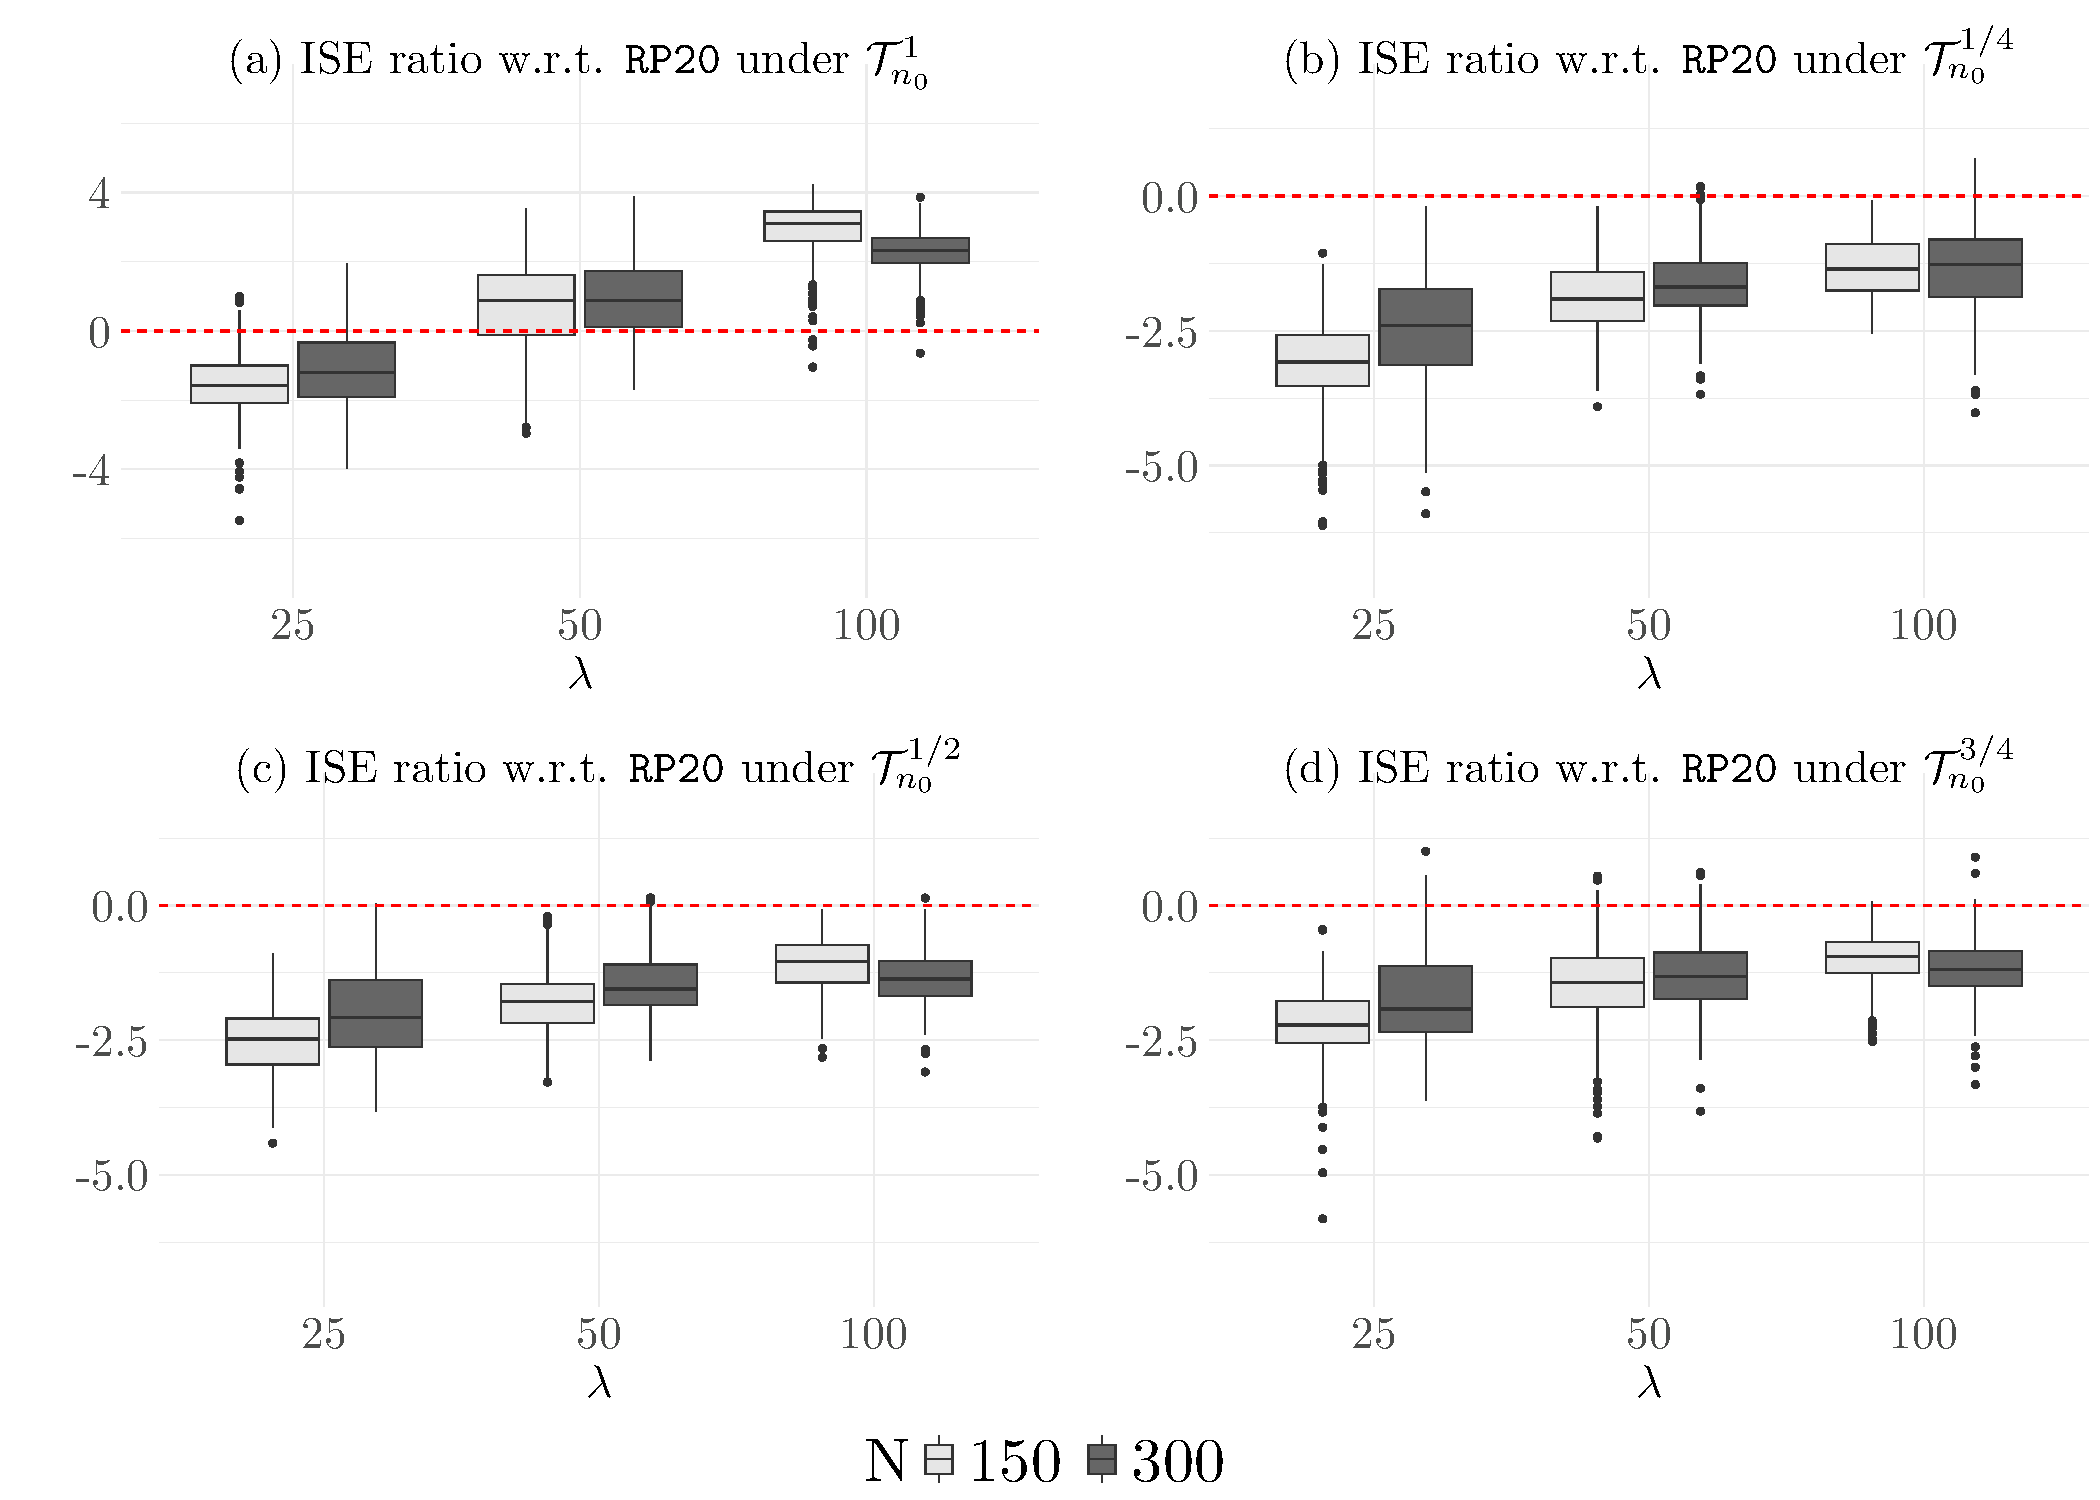
\includegraphics[width=0.9\textwidth]{./figures/blup/log_ise_ratio_blup_over_RP20_new_design_all.pdf}
	\caption{\small Boxplots of the $\log$ ISE ratios of the adaptive BLUP relative to \texttt{RP20} for predicting the last curve, with available observations in $(0, 1]$, $(0, 1/4]$, $(0, 1/2]$, and $(0, 3/4]$, respectively.}
	\label{fig:ise_ratio_blup_rp}
\end{figure}

Recall that the \texttt{RP20} method is a BLUP-based approach, where the mean is estimated using a local linear smoother and the lag-$\ell$ (auto)covariance function is estimated using a local linear surface smoother (off-diagonal, when $\ell = 0$) and a local quadratic smoother (on the diagonal, when $\ell = 0$). Smoothing bandwidths are selected via $K$-fold cross-validation coupled with Bayesian optimisation (implemented in MATLAB). Observations are randomly sampled on a regular grid of 241 points, and B-spline projections are used to reduce the computational time during optimisation.

Figure~\ref{fig:ise_ratio_blup_nw} presents boxplots of the logarithm of the ISE ratios of the adaptive BLUP relative to the NW estimator. These plots show that the adaptive BLUP generally outperforms the NW estimator, with the $\log$-relative gain tending to zero as $\lambda$ increases. When $\lambda \in \{25, 50\}$, the adaptive BLUP clearly provides better performance. However, for $\lambda = 100$, the NW estimator becomes more accurate and tends to perform similarly to the adaptive BLUP. This is likely due to the decrease in the mean squared error of the NW estimator as $\lambda$ increases, which improves its ability to reconstruct the curves effectively.

Figure~\ref{fig:ise_ratio_blup_rp} shows the boxplots of the $\log$ ISE ratios of the adaptive BLUP relative to the \texttt{RP20} method under the four scenarios $\alpha = 1, 1/4, 1/2$, and $3/4$. In the full-observation case ($\alpha = 1$), the adaptive BLUP outperforms \texttt{RP20} when $\lambda = 25$, although this advantage diminishes as $N$ increases. However, for $\lambda \in \{50, 100\}$, \texttt{RP20} yields better performance than the adaptive BLUP (see Figure~\ref{fig:ise_ratio_blup_rp}-(a)). In contrast, in the partial-observation scenarios with $\alpha \in \{1/4, 1/2, 3/4\}$, the adaptive BLUP consistently outperforms \texttt{RP20} across all considered combinations of $(N, \lambda)$, as illustrated in Figures~\ref{fig:ise_ratio_blup_rp}-(b), (c), and (d), respectively.


%\FloatBarrier

\subsection{Real data application}
We consider the prediction of daily Facebook stock volume curves. The dataset, available at \url{https://firstratedata.com/}, contains one-minute time-frame records of the stock price and volume. We extract observations from 1 January 2021 to 31 March 2022, using only the market’s regular trading hours, from 9:30~a.m to 4:00~p.m.

We construct daily stock return curves as the difference between the logarithm of the price at each time during the day and the opening price at 9:30~a.m. We are interested in predicting the traded volume when the absolute value of the return exceeds 0.5\%. Thus, for each day, we retain only the stock volume observations where the absolute return is greater than 0.5\%. The resulting daily volume curves are observed at random times between 9:30~a.m. and 4:00~p.m., with a maximum of 390 points per curve, corresponding to the total number of minutes during regular trading hours. The observation times are normalised to the interval $(0,1]$. It is worth noting that traded volume is typically very high near the market’s close; to mitigate the impact of extreme values, we exclude any volume observations above the 97.5th percentile of the entire sample.

Figure~\ref{fig:facebook_volume_last_curves} shows the last four curves in the time series. Note that, due to the return threshold, a curve may have no observations satisfying the condition on a given day. Such cases account for fewer than 10\% of all days and, therefore, we neglect the effect of this missingness. The final dataset consists of 284 curves with an average of 282 points per curve.

\begin{figure}[h]
	\centering
	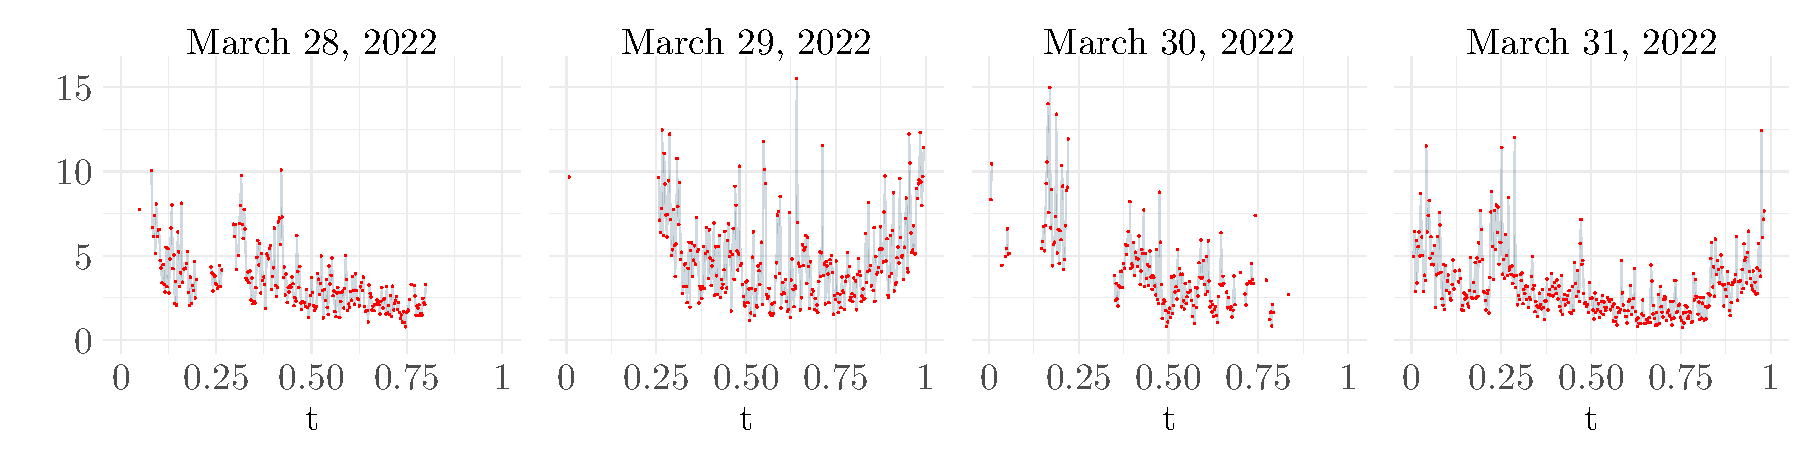
\includegraphics[width=\textwidth]{./figures/blup/Facebook_volume_4last_curves.pdf}
	\caption{\small Observation points for the last four daily Facebook stock volume curves in the dataset, with values normalised by $10^4$. Dots indicate the observation points, while the shaded lines illustrate the pattern between them.}   
	\label{fig:facebook_volume_last_curves}
\end{figure}

To assess the empirical autoregressive structure, we estimate the lag-$1$ FACF using \eqref{eq:blup:facf}, obtaining a value of $0.31$. This provides evidence that the autocovariance-related blocks in $\VV_{n_0}$ are non-negligible, indicating that the lagged curve contributes meaningfully to the adaptive BLUP. Moreover, this estimated FACF falls within the empirical distribution of lag-$1$ FACF values observed in our simulation study (see Figure~\ref{fig:conso_lag1_facf}).
 
Figure~\ref{fig:facebook_real_data_blup} presents a comparison between the adaptive BLUP predictions and the true stock volume curve to be predicted, together with a 95\% pointwise confidence interval. The comparison is performed under three scenarios, in which the available observations for the curve to be predicted are restricted to the interval $(0, \alpha]$ with $\alpha \in \{1/4, 1/2, 3/4\}$. Across these scenarios, the adaptive BLUP effectively captures local irregularities and demonstrates satisfactory predictive performance.

\begin{figure}[h]
	\centering
	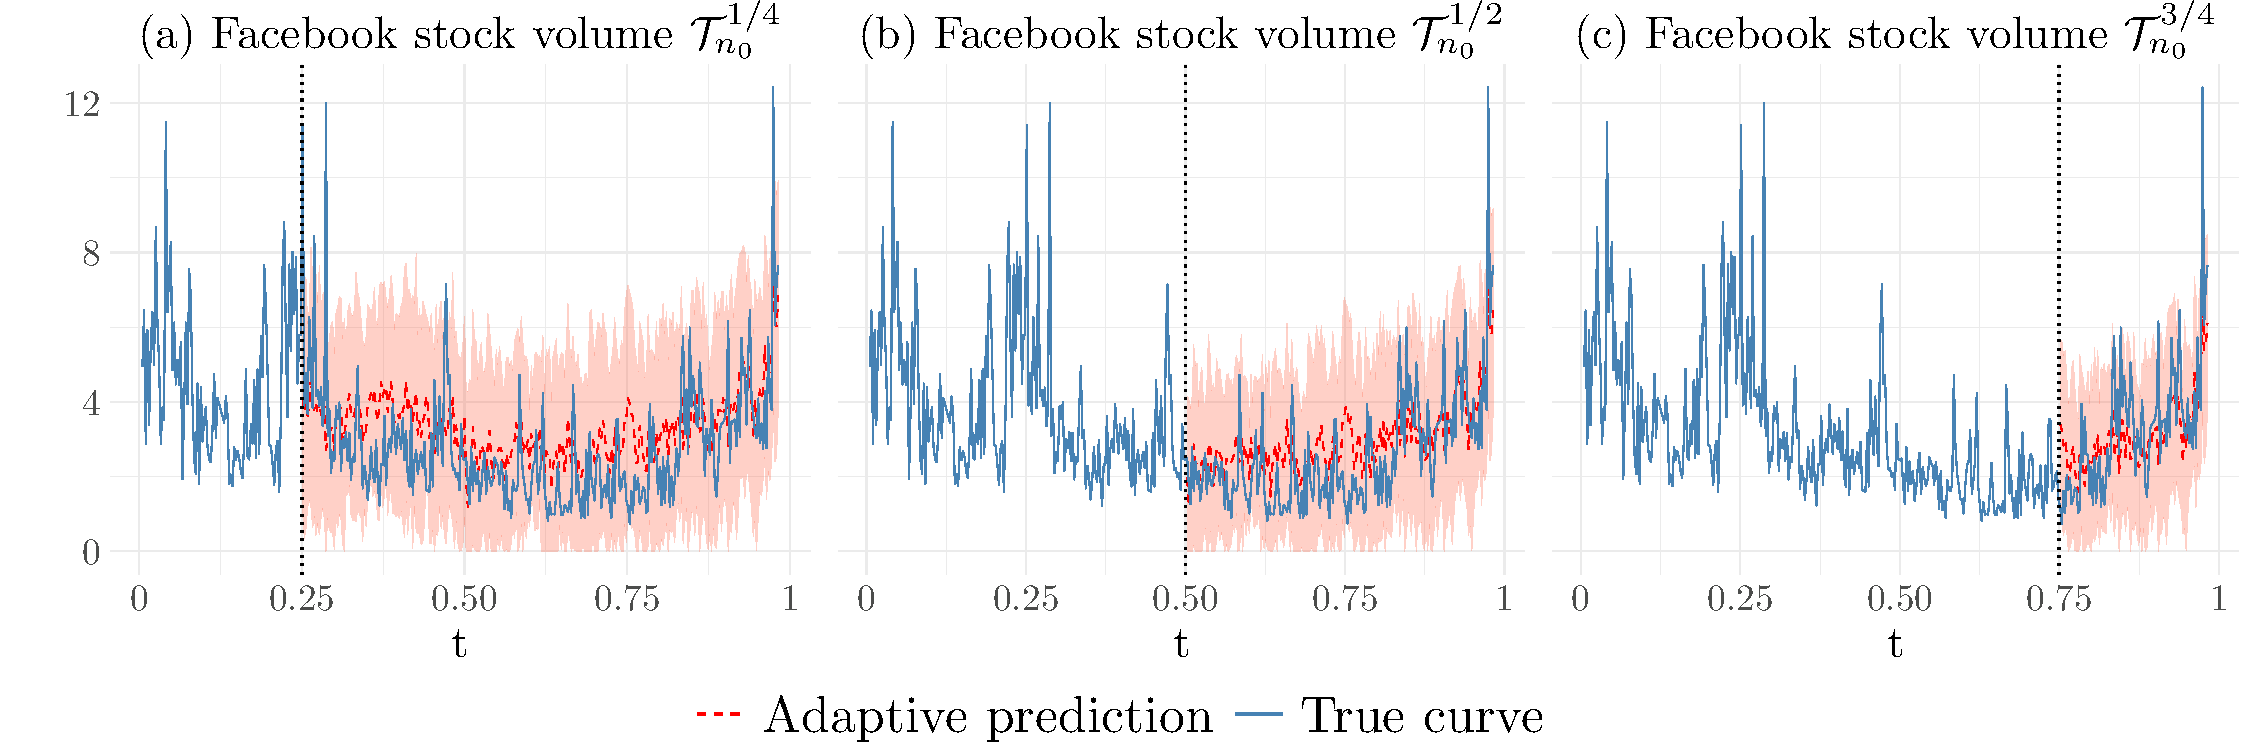
\includegraphics[width=\textwidth]{./figures/blup/Facebook_stock_volume_adaptive_pred_with_conf_band.pdf}
	\caption{\small Predictions of the last Facebook stock volume curve under scenarios where observations are available in $(0, 1/4]$, $(0, 1/2]$, and $(0, 3/4]$, respectively. The solid line shows the true curve, the dashed line shows the predicted curve, and the shaded band indicates the 95\% pointwise confidence interval. Stock volume values are normalised by $10^4$.}   
	\label{fig:facebook_real_data_blup}
\end{figure}



%%%%%%%%
%% Electricity forecasting
%%%%%%%%

%Forecasting electricity consumption and production is essential for maintaining the balance of the electricity system, as it helps to significantly reduce the costs associated with storage and overproduction. Accurate forecasting is therefore a major economic challenge, especially in sectors such as hydropower and photovoltaics, where production varies significantly throughout the day due to weather dependencies. Functional time series provide an effective framework for modelling such trajectories, especially when the forecasting method adapts to the regularity of the underlying process, as in the case of adaptive BLUP. 
%
%\begin{figure}[h]
%	\centering
%	
\includegraphics[width=\textwidth]{Chapitre3/figures/blup/plot_adaptive_blup_energy_with_conf_band.pdf}
%	\caption{\small Electricity curve prediction. The first row shows the results for the consumption curves, the second for the photovoltaic curves, and the third for the hydroelectric curves. Each column corresponds to reconstructing the solid curve with available observations restricted to the intervals $(0, 1/4]$, $(0, 1/2]$, and $(0, 3/4]$, respectively. The shaded bands indicate the 95\% pointwise confidence intervals.}   
%	\label{fig:real_data_blup}
%\end{figure}
%
%To illustrate this approach, we analyse daily curves of national electricity consumption in France, along with daily production curves for photovoltaic and hydroelectric electricity, obtained from the ODRÉ platform \citep{odre_data}. The dataset for consumption spans the period from June to September 2024 and comprises $122$ daily curves. Each consumption curve is recorded at $96$ equally spaced time points, with measurements taken every $15$ minutes. The photovoltaic production dataset also covers the period from June to September 2024 and includes $122$ daily curves. Since photovoltaic output depends on sunlight, observations are restricted to $61$ time points recorded every $15$ minutes between 4~a.m.\ and 7~p.m.\ on the same $122$ days. The hydroelectricity production dataset consists of $152$ daily curves observed at $96$ equally spaced time points every $15$ minutes, collected between November 2023 and March 2024. All values for each type of curve are normalised to the interval $[0,1]$ by scaling them with the maximum observed production value.
%
%To assess the empirical autoregressive structure, we estimate the lag-$1$ FACF using \eqref{eq:blup:facf}, obtaining values of $0.42$, $0.44$, and $0.36$ for the consumption, photovoltaic production, and hydroelectric production curves, respectively. These estimates provide evidence that the autocovariance-related blocks in $\VV_{n_0}$ are non-negligible, which indicates that the lagged curve contributes meaningfully to the adaptive BLUP. Moreover, each estimated FACF falls within the empirical distribution of lag-$1$ FACF values observed in our simulation study (see Figure~\ref{fig:conso_lag1_facf}).
%
%Figure~\ref{fig:real_data_blup} presents a comparison between the adaptive BLUP predictions and the actual curves to be predicted for the three types of curve sets, together with the 95\% pointwise confidence interval. The comparison is conducted under scenarios where the available observations are restricted to the interval $(0, \alpha]$, with $\alpha \in \{1/4, 1/2, 3/4\}$. Across all curve types and observation scenarios, the adaptive BLUP effectively captures local irregularities and demonstrates satisfactory predictive performance.



\FloatBarrier


\newpage


\appendix

\section{Proofs associated to the Regularized linear predictor}

\begin{proof}[Proof of Proposition \ref{prop:tikhonov}]
For simplicity, we write $\mathfrak{X}^{(M_{n_0})}_{n_0+1}(t )$ instead of $\mathfrak{X}^{(M_{n_0})}_{n_0+1}(t;\alpha,\sigma^2 \Dd_{n_0} )$. 
We define the $(M_{n_0}\times M_{n_0})-$matrices 
$$ 
\mathcal A _{M_{n_0}} = \alpha I_{M_{n_0}} +  \sigma^2  \Dd_{n_0}, \qquad  
R_{n_0,M_{n_0}} = \left(\Pi_{n_0,0}\Pi_{n_0,0}^\star + \mathcal A_{M_{n_0}} \right)^{-1},
$$ 
and let $f=X_{n_0}-\mu$ hereafter.  Notice that $R_{n_0,M_{n_0}}$ is symmetric with positive eigenvalues, and the largest one, denoted by $\lambda_{\max} (R_{n_0,M_{n_0}})$  is bounded by $1/\alpha$.
% the spectral norm $\rho(R_{n_0,M_{n_0}})$ of $R_{n_0,M_{n_0}}$ is bounded $1/\alpha$.
We rewrite the Tikhonov regularized predictor as the sum of two terms,
\begin{align*}
	\mathfrak{X}^{(M_{n_0})}_{n_0+1,\alpha}(s)&= \mu(s) + \left\{\Pi_{n_0,1}^\star R_{n_0,M_{n_0}}( \Dd_{n_0}^{1/2}\mathbf{Y}_{n_0}-\Pi_{n_0,0}\mu)\right\}(s) = A_{n_0,\alpha}(s;f) + B_{n_0,\alpha}(s), \qquad s\in I,
\end{align*}
where
$$
A_{n_0,\alpha}(s;f) = \mu(s) + \left[\Pi_{n_0,1}^\star \left\{R_{n_0,M_{n_0}}\Pi_{n_0,0}(X_{n_0}-\mu)\right\}\right](s) =C_{n_0,1}(t)^\top  \Dd_{n_0}^{1/2} R_{n_0,M_{n_0}}  \Pi_{n_0,0}(X_{n_0}-\mu),
$$
and 
$$
B_{n_0,\alpha}(s) = \left[\Pi_{n_0,1}^\star \left\{R_{n_0,M_{n_0}}\epsb_{n_0}\right\}\right](s)=  C_{n_0,1}(s)^\top  \Dd_{n_0}^{1/2} R_{n_0,M_{n_0}}  \Dd_{n_0}^{1/2} \epsb_{n_0} .
$$

First, we derive a bound for $\EEMT(\|B_{n_0}\|_{\infty} )$.
%Let 
%$$
%c_1^{(n_0)}(s)=\mathcal R_n^{1/2}\big(c_1(T_{n_0,1},t),\ldots,c_1(T_{n_0,M_{n_0}},t)\big)^\top\in\RR^{M_{n_0}}.
%$$
Since \assrefH{H:model:epsni}, we get,
\begin{align}\label{bound_Bn0}
\EEMT(\|B_{n_0}\|^2_{\infty}) &= \sigma^2\Big\| C_{n_0,1}(\cdot)^\top \Dd^{1/2}_{n_0} R_{n_0,M_{n_0}} \Dd_{n_0} R_{n_0,M_{n_0}}\Dd^{1/2}_{n_0} C_{n_0,1}(\cdot )\Big\|_\infty \\
&  = \sigma^2 \Big\|  \mathrm{Tr}\left(R_{n_0,M_{n_0}} \Dd_{n_0} R_{n_0,M_{n_0}}\  \Dd^{1/2}_{n_0}C_{n_0,1}(\cdot)C_{n_0,1}(\cdot)^\top \Dd^{1/2}_{n} \right) \Big\|_\infty\\
&\leq  \sigma^2\lambda^2_{\max} (R_{n_0,M_{n_0}} \Dd_{n_0} R_{n_0,M_{n_0}}) \Big\| \mathrm{Tr}\left(\Dd^{1/2}_{n_0} C_{n_0,1}(s)C_{n_0,1}(s)^\top\Dd^{1/2}_{n_0} \right) \Big\|_\infty \\
& \leq \frac{\sigma^2 \max_{i}\varrho_{n_0,i}}{\alpha^2} \Big\|  \sum_{j=1}^n \varrho_{n,j} C_1(s,T_{n_0,j})^2 \Big\|_\infty \\
& \leq  \sigma^2\|c_1\|^2_\infty \frac{\max_{i}\varrho_{n_0,i} }{\alpha^2 }.
%\xrightarrow[M_{n_0}\to\infty]{a.s.} 0.   
\end{align}
For the second inequality in \eqref{bound_Bn0} we use the fact that 
$$
\lambda^2_{\max} (R_{n_0,M_{n_0}} \Dd_{n_0} R_{n_0,M_{n_0}})\leq \max_{i}\varrho_{n_0,i} \lambda^2_{\max} (R_{n_0,M_{n_0}})^2\leq \max_{i}\varrho_{n_0,i} /\alpha^2.
$$ 
Indeed, for any unit vector $u\in\RR^{M_{n_0}}$, $u^\top R_{n_0,M_{n_0}} \Dd_{n_0} R_{n_0,M_{n_0}} u = v^\top  \Dd_{n_0} v$, where $v=R_{n_0,M_{n_0}} u.$ 
Since $ \Dd_{n_0}$ is a diagonal matrix with diagonal terms in $(0,1),$
$$
	u^\top R_{n_0,M_{n_0}} \Dd_{n_0} R_{n_0,M_{n_0}} u = \sum_{i=1}^n \varrho_{n_0,i} v_i^2 \leq \max_{i}\varrho_{n_0,i} \| R_{n_0,M_{n_0}} u \|_2^2 \leq \max_{i}\varrho_{n_0,i} \lambda^2_{\max} (R_{n_0,M_{n_0}})^2 \|u\|_2^2.
$$
The bound on $\lambda^2_{\max}$ follows. As a consequence of \eqref{bound_Bn0}, the rate of convergence to zero for $\EEMT(\|B_{n_0}\|^2_{\LL^2(I)}) $ is bounded by $\alpha^{-2}\max_{i}\varrho_{n_0,i} $. 
In the case of common design, $\max_{i}\varrho_{n_0,i} = M_{n_0}^{-1}$.
\color{red}
With independent design,  $\varrho_{n_0,i} = \{M_{n_0} \,\widehat{g}_{n_0,i}(T_{n_0,i})\}^{-1}$, it holds 
$$
\max_{1\leq i \leq M_{n_0}} \varrho_{n_0,i} = \frac{1}{M_{n_0}} \cdot \max_{1\leq i \leq M_{n_0}} \frac{1}{\widehat{g}_{n_0,i}(T_{n_0,i})}.
$$
By \cite{gine_2002}, the leave-one-out Parzen–Rosenblatt estimator satisfies
$$
\sup_{1\leq i\leq M_{n_0}}|\{g(T_{n_0,i})/\widehat g_{n_0,i}(T_{n_0,i})\} - 1 | \rightarrow 0,\quad \text{almost surely}.
$$
Since $g_{\min} := \inf_{t\in I} g(t) > 0$ by assumption \assrefH{H:model:Tni}, this uniform convergence implies that, almost surely for $M_{n_0}$ large enough, $\widehat{g}_{n_0,i}(T_{n_0,i}) \geq g_{\min}/2$ for all $1\leq i \leq M_{n_0}$
Consequently,$\max_{1\leq i \leq M_{n_0}} \varrho_{n_0,i} \leq \frac{2}{M_{n_0}\, g_{\min}},$ which is of order $\Oo_{\PP}(M_{n_0}^{-1})$, matching the common design case. We conclude that in both cases,
We deduce that 
\begin{equation}\label{error_term_contrib}
	\EEMT(\|B_{n_0}\|^2_{\LL^2(I)})  =  \alpha^{-2}O_{\mathbb P}\big( M_{n_0}^{-1}\big).
\end{equation}
\color{black}

To study $A_{n_0}$, 
let $\boldsymbol{\beta}_{n_0}  = (\beta_{n_0,i})= R_{n_0,M_{n_0}}\Pi_{n_0,0}f \in \RR^{M_{n_0}}$ so that 
$$
A_{n_0}(s;f) - \mu(s) = \left\{\Pi_{n_0,1}^* \boldsymbol{\beta}_{n_0}\right\}(s) .
%= \frac{1}{M_{n_0}}\sum_{i=1}^{M_{n_0}} \alpha_{n_0,i}\,c_1(t,T_{n_0,i}).
$$
By definition, the vector $\boldsymbol{\beta}_{n_0}$ is then the unique solution of 
\begin{equation}\label{eq:proof:tikhonov:alpha0}
\left(\Pi_{n_0,0}\Pi_{n_0,0}^* + \mathcal A_{M_{n_0}}  \right)\boldsymbol{\beta}_{n_0} =  \Dd_{n_0}^{1/2} \big(f(T_{n,1}),\ldots,f(T_{n,M_{n_0}})\big)^\top.
\end{equation}
We prove below that with the continuous random function $\mathfrak h=(C_0+\alpha\,\mathrm{Id})^{-1}f$ we get 
\begin{equation}\label{beta_proba_cvg}
\| \boldsymbol{\beta}_{n_0} - \Pi_{n_0,0} \mathfrak h\|_{2} \to 0 \qquad \text{  in probability}.
\end{equation}
For any $1\leq  i\le M_{n_0}$, let 
$$
\delta_{n_0,i} =  {\beta}_{n_0,i} - \sqrt{\varrho_{n_0,i}}\,  \mathfrak h(T_{n_0,i}) \quad \text{ and } \quad \boldsymbol{\delta}_{n_0} = (\delta_{n_0,i})\in\RR^{M_{n_0}}.
$$ 
such that $\boldsymbol{\delta}_{n_0} = \boldsymbol{\beta}_{n_0} - \Pi_{n_0,0} \mathfrak h $. Recall that, by definition, the function $\mathfrak h$ satisfies,
\begin{equation}\label{eq:proof:tikhonov:h}
\int_0^1 \mathfrak h(s)c_0(s,T_{n_0,i})ds + \alpha \mathfrak h(T_{n_0,i}) = f(T_{n_0,i}), \quad i=1,\ldots,M_{n_0}.
\end{equation}
Let $\mathbf{r}_{n_0}= (r_{n_0,i}):=R_{n_0,M_{n_0}}^{-1}\boldsymbol{\delta}_{n_0}$. Then we have
\begin{align*}
\mathbf{r}_{n_0} = \Pi_{n_0,0}f  - \Pi_{n_0,0}\left[\Pi_{n_0,0}^\star\Pi_{n_0,0} \mathfrak h\right] - \alpha \Pi_{n_0,0} \mathfrak h - \sigma^2  \Dd_{n_0} \Pi_{n_0,0} \mathfrak h,
\end{align*}
\textit{i.e.} for $i=1,\ldots M_{n_0},$
\begin{align*}
r_{n_0,i} =  \sqrt{\varrho_{n_0,i}} \int_0^1 \mathfrak h(s)c_0(s,T_{n_0,i})ds  -  \sqrt{\varrho_{n_0,i}} \int_0^1 \mathfrak h(s)c_0(T_{n_0,i},s)dQ_{n_0}(s) - \sigma^2 \varrho_{n_0,i} \sqrt{\varrho_{n_0,i}} \,\mathfrak h(T_{n_0,i}).
\end{align*}
So we get that,
\begin{align*}
\|\mathbf{r}_{n_0}\|^2_2 &\leq 2\sum_{i=1}^{M_{n_0}} \varrho_{n_0,i} \left(\int_0^1 \mathfrak h(s)c_0(s,T_{n_0,i})ds - \int_0^1 \mathfrak h(s)c_0(s,T_{n_0,i})dQ_{n_0}(s)\right)^2+2 \color{blue} \sigma^2 \color{black}  \sum_{i=1}^{M_{n_0}} \varrho_{n_0,i}^3 \mathfrak h^2(T_{n_0,i})\\
&\leq  2 \sum_{i=1}^{M_{n_0}} \varrho_{n_0,i} \left(\int_0^1 \mathfrak h(s)c_0(s,T_{n_0,i})ds - \int_0^1 \mathfrak h(s)c_0(s,T_{n_0,i})dQ_{n_0}(s)\right)^2+2 \color{blue} \sigma^2  \{\|\mathfrak h\|_\infty \max_i \varrho_{n_0,i} \}^2\color{black}\\
&= :  2 \sum_{i=1}^{M_{n_0}} \varrho_{n_0,i} \left(\widetilde I\big(\varphi_i \big) - I\big(\varphi_i\big) \right)^2+2 \color{blue} \sigma^2  \{\|\mathfrak h\|_\infty \max_i \varrho_{n_0,i} \}^2\color{black},
\end{align*}
where $\varphi_i(\cdot)  = \mathfrak h(\cdot) c_0(\cdot, T_{n_0,i} ) $ and, for any $\varphi :I \rightarrow \RR$,  
$$
\widetilde I(\varphi)  =  \int_0^1 \varphi (s)dQ_{n_0}(s) \qquad\text{and}  \qquad  I(\varphi) = \int_0^1 \varphi (s)ds.
$$
The cases common and independent design have to be treated separately. 


\emph{Independent design}. 
\color{red} 
Using the decomposition of $\widetilde I(\varphi) - I(\varphi)$ as on \citet[p. 2196]{DP2016}, we can write it as
\begin{equation}\label{our_decom}
 \widetilde I(\varphi_i) - I(\varphi_i) =  R_{0,i} + R_{1,i} + R_{2,i}^{(1)} + R_{2,i}^{(2)} + R_{5,i},
\end{equation}
where  $R_{1,i}$, $R_{2,i}^{(1)}$ and $R_{2,i}^{(2)}$ are  the bias terms (with $R_{2,i}^{(1)} + R_{2,i}^{(2)}$ corresponding to  $R_2$ in the decomposition used by \citet[Step 3, p. 2191]{DP2016}). 
In our case, let $R_{2,i}^{(2)}$ be the term with the rate depending on the smoothness of $\varphi_i$, while the rates of $R_{1,i}$ and $R_{2,i}^{(1)}$ depend on the smoothness of the density $g$.
Following the lines of the proof of \citet[Theorem 1-(i)]{DP2016}), the term $|M_{n_0}^{1/2}R_{2,i}^{(2)}|$ can be bounded by a product between a constant depending only on $g$ and the kernel $K$, the Hölder constant of $\varphi_i$ and $h^\beta$, see \citet[Eq. (20) in Lemma 6]{DP2016} and the decomposition in the last display before \emph{Step 4} in \citet[on p. 2192]{DP2016}.
\color{purple}
La régularité est $\min(\beta,r)$~?
\color{red} 
Meanwhile, the sum $|R_{1,i}+R_{2,i}^{(1)}|$ can be written under the form of a product between  $(\|\varphi_i\|_\infty +1)$, the uniform bound of $g^{(r)}$ times $h^r$, and a constant depending only on $g$ and $K$, see \citet[Eq. (18) and (19) in Lemma 6]{DP2016} and the bounds on $R_2$ in \citet[p. 2192]{DP2016}.
Moreover,  the Hölder constant of $\varphi_i$ is bounded by  \textcolor{red}{$ \alpha^{-1} \|c_0\|_\infty \mathfrak L_{n_0} (\beta) + \alpha^{-1} \|f\|_\infty \sqrt{\|c_0\|_\infty}\sqrt{\EE \mathfrak L_{n_0} (\beta)^2}$.} 
Then, since  both $\mathfrak L_{n_0} (\beta) $ and $\|X_{n_0}-\mu\|_\infty$ are independent of the design and have finite expectation, integrating with respect $X_{n_0}$, we deduce 
\begin{equation}\label{CP_bound2a}
\EEMT\left[ \sum_{i=1}^{M_{n_0}} \varrho_{n_0,i} \left( R_{1,i} + R_{2,i}^{(1)} + R_{2,i}^{(2)} \right)^2 \right] = \alpha^{-2}O_{\mathbb P}(h^{2r}+M^{-1}_{n_0}h^{2\beta}).
\end{equation}

To bound the last term $\mathcal{V}_{M_{n_0}} (\varphi_i)=R_0+R_5$ in the decomposition \eqref{our_decom}, we first note that by the definition of the terms in the decomposition, 
$$
\forall i,\quad |\mathcal V_{M_{n_0}} (\varphi_i)|\leq \alpha^{-1}  \|f \|_\infty \sup_{\phi\in \mathcal S(\mathfrak h)} \left| \mathcal V_{M_{n_0}}(\phi)\right|,
$$
where 
$$
\mathcal S (\mathfrak h)= \{\phi= \alpha \mathfrak h \|f \|_\infty ^{-1}c_0(\cdot,t), t\in I\}.
$$
\color{black}
Note that $\|\phi\|_\infty \leq \|c_0\|_\infty$, $\forall \phi\in \mathcal S (\mathfrak h)$. 
\cite{DP2016} derive the rate $O_{\mathbb P}(M_{n_0}^{-1} h^{-1})$ for $\mathcal V_{M_{n_0}}(\phi)$ with a single $\phi$.
In a closely related context, \cite{CP2018} extended the result and derived the  bound $O_{\mathbb P}(\textcolor{red}{\sqrt{M_{n_0}^{-1} h^{-1}\log(1/h)}})$ for $\mathcal V_{M_{n_0}}(\cdot)$ uniformly over a countable VC class. The arguments of \cite{CP2018}, based on exponential bounds (depending only on the complexity and the envelope of the class, and not on the class itself) for deviations of  empirical processes and degenerate $U$-processes, can also be applied in our case.
\color{red}
Taking $\mathcal{S}_{\mathbb{Q}}(\mathfrak{h}) = \{\alpha\mathfrak{h}\|f\|_\infty^{-1}c_0(\cdot,t),\, t\in\mathbb{Q}\cap(0,1)\}$ as a countable subset of $\mathcal{S}(\mathfrak{h})$, $\mathcal{S}(\mathfrak{h})
S(h)$ is countably approximable in the sense of \citet{major2006estimate}.
Indeed $t\mapsto c_0(s,t)$ is continuous uniformly in $s$, the map $t\mapsto \mathcal{V}_{M_{n_0}}(\phi_t)$ is p.s. continuous, so that the supremum over $t\in I$ equals p.s. the supremum over $t\in\mathbb{Q}\cap(0,1)$.
Moreover, by the uniform Hölder continuity of $c_0(s,\cdot)$ (uniformly in $s$), the class $\mathcal{S}_{\mathbb{Q}}(\mathfrak{h})$ is of VC-type with complexity constants independent of $M_{n_0}$ and $X_{n_0}$ (see Lemma~\ref{lem:vc_bounded_mult}).
Applying the nonasymptotic bound of \citet[Lemma 3]{CP2018}, which extends the concentration inequality of Major (2006) to degenerate $U$-processes indexed by VC-type classes, we obtain
$$
\sup_{\phi \in \mathcal{S}(\mathfrak{h})} |\mathcal{V}_{M_{n_0}}(\phi)| = O_{\mathbb{P}}\!\left(\sqrt{M_{n_0}^{-1}h^{-1}\log(1/h)}\right)
$$
Since $\|X_{n_0}-\mu\|_\infty$ is integrable and the exponential deviation bound for the supremum above depends on $X_{n_0}$ only through $\|f\|_\infty$ (via the envelope of the class), we may integrate with respect to $X_{n_0}$ to deduce
\begin{equation}\label{CP_bound2b}
\EEMT\left[ \sum_{i=1}^{M_{n_0}} \varrho_{n_0,i} \mathcal V_{M_{n_0}}(\varphi_i) ^2 \right] \leq \alpha^{-2} O_{\mathbb P}\big(\{M_{n_0}^{-1} h^{-1}\log(1/h)\}^2\big).
\end{equation} 
\color{black}
 
%In a closely related context, \cite{CP2018} extended the result and derived the  bound $O_{\mathbb P}(\textcolor{red}{\sqrt{M_{n_0}^{-1} h^{-1}\log(1/h)}})$ for $\mathcal V_{M_{n_0}}(\cdot)$ uniformly over a countable VC class. The arguments of \cite{CP2018}, based on exponential bounds (depending only on the complexity and the envelope of the class, and not on the class itself) for deviations of  empirical processes and degenerate $U$-processes, can also be applied in our case. Using the Hölder continuity of the functions $c_0(s,\cdot)$ (uniformly with respect to $s$), it is easy to check that the set of functions $\{ c_0(s,\cdot), s\in I\}$ is a VC class.  Next, it is easy to check the VC preservation for the class  $\mathcal S (\mathfrak h)$; see Lemma \ref{lem:vc_bounded_mult}. Moreover, the complexity of  $\mathcal S (\mathfrak h)$ does not depend on  $X_{n_0}-\mu$. 
%Since $\|X_{n_0}-\mu\|_\infty$ is integrable and the deviations of $\sup_{\phi\in \mathcal S(\mathfrak h)} \left| \mathcal V_{M_{n_0}}(\phi)\right|$ admit an exponential bound which does not depend on $X_{n_0}$, we deduce that 
%\begin{equation}\label{CP_bound2b}
%\EEMT\left[ \sum_{i=1}^{M_{n_0}} \varrho_{n_0,i} \mathcal V_{M_{n_0}}(\varphi_i) ^2 \right] \leq \alpha^{-2} O_{\mathbb P}\big(\{M_{n_0}^{-1} h^{-1}\log(1/h)\}^2\big).
%\end{equation}


\emph{Common design}. In this case we simply have to bound the error of a standard Riemann sum when the integrand is Hölder continuous. The details are omitted. 


Now, using the bound on the spectral norm of $R_{n_0,M_{n_0}}$, we get 
\begin{equation}
\|\boldsymbol{\delta}_{n_0}\|_2^2 = \| \boldsymbol{\beta}_{n_0} - \Pi_{n_0,0} \mathfrak h\|^2_{2}  \leq \alpha^{-2} \|\mathbf{r}_{n_0}\|_2^2 .
\end{equation}
Finally, by Cauchy-Schwarz inequality, for any $s\in I$ we get 
\begin{align}\label{A_bound_fin}
\left|\{A_{n_0}(s;f) - \mu(s)\} - \Pi_{n_0,1}^\star \Pi_{n_0,0} h(s)\right| &= \left|C_{1,n}(s)^\top  \Dd_{n_0}^{1/2}(\boldsymbol{\beta}_{n_0} - \Pi_{n_0,0} h)\right|\\ 
&\leq \| \Dd_{n_0}^{1/2}C_{1,n}(s)\|_2 \| \boldsymbol{\beta}_{n_0} - \Pi_{n_0,0} h\|_{2},\\
&\leq \|c_1\|_\infty \| \boldsymbol{\beta}_{n_0} - \Pi_{n_0,0} h\|_{2},
\end{align}
and the last bound does not depend on $s$. 
Combining \eqref{CP_bound2a}, \eqref{CP_bound2b} and \eqref{A_bound_fin}, we get \eqref{beta_proba_cvg}.
\end{proof}




\begin{lemma}	\label{lem:vc_bounded_mult}
	Let $\Theta \subset \mathbb{R}^d$ be compact and let $\mathcal{F} = \{f_\theta : \theta \in \Theta\}$
	be a class of uniformly bounded functions on $[0,1]$ satisfying, for some $L > 0$
	and $\alpha \in (0,1]$,
	\begin{equation}
		\label{eq:holder_param}
		\|f_{\theta_1} - f_{\theta_2}\|_\infty \leq L\,|\theta_1 - \theta_2|^\alpha,
		\qquad \theta_1, \theta_2 \in \Theta.
	\end{equation}
	Let $\mathfrak g : [0,1] \to \mathbb{R}$ be measurable with $\|\mathfrak g\|_\infty \leq M$. Then, for all
	$\varepsilon > 0$ and all probability measures $Q$ on $[0,1]$,
	\begin{equation}
		\label{eq:covering_gF}
		N\!\left(\varepsilon,\; \mathfrak g\mathcal{F},\; L^2(Q)\right)
		\;\leq\;
		\left(\frac{c_\Theta\, ML}{\varepsilon}\right)^{d/\alpha},
	\end{equation}
	where $c_\Theta := \bigl(2\,\mathrm{diam}(\Theta)\bigr)^\alpha$ depends only on
	$\alpha$ and $\Theta$.
	In particular, $\mathfrak g\mathcal{F}$ is a VC class with metric entropy exponent $d/\alpha$,
	equal to that of $\mathcal{F}$.
\end{lemma}

\begin{proof}[Proof of Lemma \ref{lem:vc_bounded_mult}]
	Set $\delta := \bigl(\varepsilon/(ML)\bigr)^{1/\alpha}$.
	A standard volumetric argument yields a $\delta$-net
	$\{\theta_1,\ldots,\theta_N\} \subset \Theta$ with
	\[
	N \;\leq\; \left(\frac{2\,\mathrm{diam}(\Theta)}{\delta}\right)^d
	\;=\; \left(\frac{c_\Theta\,ML}{\varepsilon}\right)^{d/\alpha}.
	\]
	For any $\theta \in \Theta$, pick $\theta_i$ with $|\theta - \theta_i| \leq \delta$. Then
	\[
	\|gf_\theta - gf_{\theta_i}\|_\infty
	\;\leq\; M\,\|f_\theta - f_{\theta_i}\|_\infty
	\;\leq\; ML\,\delta^\alpha
	\;=\; \varepsilon.
	\]
	Hence $\{\mathfrak gf_{\theta_1},\ldots,\mathfrak gf_{\theta_N}\}$ is an $\varepsilon$-cover of $\mathfrak g\mathcal{F}$
	in $L^\infty$, and \eqref{eq:covering_gF} follows since
	$\|\cdot\|_{L^2(Q)} \leq \|\cdot\|_\infty$ for any probability measure $Q$.
\end{proof}

\begin{proof}[Proof of Proposition \ref{prop:unif:conv}]
We can decompose $\widehat{\Xf}_{n_0}-{\Xf}_{n_0}$ as the sum of four terms,
$$
\widehat{\Xf}_{n_0}-{\Xf}_{n_0}=A+B+C+D
$$
where
\begin{align*}
A&= \widehat{\mu}-\mu,&\qquad
B&= \widehat{\Pi}_{n_0,1}^\star \widehat{R}_{n_0}^{-1} \Pi_{n_0,0}(\widehat{\mu}-\mu),\\
C&= (\widehat{\Pi}_{n_0,1}^\star-{\Pi}_{n_0,1}^\star) \widehat{R}_{n_0}^{-1} (\Dd^{1/2}_{n_0}\Yb_{n_0}-\Pi_{n_0,0}\mu),&\qquad
D&= {\Pi}_{n_0,1}^\star (\widehat{R}_{n_0}^{-1}- {R}_{n_0}^{-1}) (\Dd^{1/2}_{n_0}\Yb_{n_0}-\Pi_{n_0,0}\mu).
\end{align*}

\medskip

Remark that,
\begin{align*}
\|\Pi_{n_0,0}(\widehat{\mu}-\mu)\|_2^2= \sum_{i=1}^{M_n}\rho_{n,i}\left(\widehat{\mu}(T_{n,i})-{\mu}(T_{n,i})\right)^2 \leq \|A\|_\infty^2.
\end{align*}
Since the largest eignevalue of $\widehat{R}_{n_0,M_{n_0}}$  is bounded by $1/\alpha$, and according to Theorem \ref{thm:mean_unif_cv} and \ref{thm:cov_unif_cv}, we have,
\begin{align*}
\|A+B\|_\infty&= \|\widehat{\mu}-\mu\|_\infty \left(1 + \alpha^{-1}(\|c_1\|_\infty + \|\widehat{c}_1-c_1\|_\infty\right).
\end{align*}

\medskip

Furthermore, we can establish that,
$$
\|\Dd^{1/2}_{n_0}\Yb_{n_0}-\Pi_{n_0,0}\mu\|_2 \leq \sqrt{2}\sqrt{\|X_{n_0}-\mu\|_\infty^2 +\sigma^2 \left(1 + \Oo_\PP\left(\max_{i}\rho_{n_0,i}\right)\right)}
$$ 
Indeed, using that $(a+b)^2\leq 2 a^2+b^2$ for $a,b\in\RR,$ we have,
\begin{align*}
\|\Dd^{1/2}_{n_0}\Yb_{n_0}-\Pi_{n_0,0}\mu\|_2^2 \leq 2 \sum_{i=1}^{M_n}\rho_{n_0,i}(X_{n_0}(T_{n_0,i})-\mu(T_{n_0,i}))^2 + 2\sigma^2\sum_{i=1}^{M_n} \rho_{n_0,i}\epsilon_{n,i}^2. 
\end{align*}
Since $\rho_{n_0,1}+\ldots+\rho_{n_0,M_{n_0}}=1,$
\begin{align*}
\sum_{i=1}^{M_n}\rho_{n_0,i}(X_{n_0}(T_{n_0,i})-\mu(T_{n_0,i}))^2 &\leq \|X_{n_0}-\mu\|_\infty^2\\ 
\EEMT\left(\sum_{i=1}^{M_n} \rho_{n_0,i}\epsilon_{n,i}^2\right)&=1 \quad\text{and}\quad
\Var_{M,T}\left(\sum_{i=1}^{M_n} \rho_{n_0,i}\epsilon_{n,i}^2 \right) \leq \max_{i} \rho_{n_0,i}.
\end{align*}
By Tchebychev inequality, we deduce that, 
$$
\sigma^2\sum_{i=1}^{M_n} \rho_{n_0,i}\epsilon_{n,i}^2 =\sigma^2\left(1 + \Oo_\PP(\max_{i} \rho_{n_0,i})\right).
$$
Then the Cauchy-Schwarz inequality implies that,
\begin{align*}
|C(t)| &\leq \|\widehat{c}_1-c_1\|_{\infty}\left\| \widehat{R}_{n_0}^{-1} (\Dd^{1/2}_{n_0}\Yb_{n_0}-\Pi_{n_0,0}\mu) \right\|_2\\
	  &\leq  \alpha^{-1}\|\widehat{c}_1-c_1\|_{\infty} \sqrt{2\|X_{n_0}-\mu\|_\infty^2 +2\sigma^2 \left(1 + \Oo_\PP\left(\max_{i}\rho_{n_0,i}\right)\right)} 
\end{align*}

\medskip

Remark that $D$ can be rewritten as,
\begin{align*}
D &= {\Pi}_{n_0,1}^\star \widehat{R}_{n_0}^{-1} ({R}_{n_0}- \widehat{R}_{n_0}) {R}_{n_0}^{-1} (\Dd^{1/2}_{n_0}\Yb_{n_0}-\Pi_{n_0,0}\mu).
\end{align*}
Using the same argument than the term $C$, we deduce that,
\begin{align*}
|D(t)| &\leq \|c_1\|_\infty \|\widehat{R}_{n_0}^{-1}\|_2 \| \Pi_{n_0,0}(\widehat{\Pi}_{n_0,0}^\star - {\Pi}_{n_0,0}^\star) + (\widehat{\sigma}-\sigma^2)\Dd_{n_0}\|_2 \| {R}_{n_0}^{-1}\|_2 \|\Dd^{1/2}_{n_0}\Yb_{n_0}-\Pi_{n_0,0}\mu\|_2\\
&\leq \|c_1\|_\infty \sqrt{2\|X_{n_0}-\mu\|_\infty^2 +2\sigma^2 \left(1 + \Oo_\PP\left(\max_{i}\rho_{n_0,i}\right)\right)} \left(\|\widehat{c}_0-c_0\|_\infty + |\widehat{\sigma}-\sigma| \max_{i}\rho_{n,i}  \right)\alpha^{-2}.
\end{align*}
\end{proof}



\section{Uniform consitent estimators}


\begin{theorem}\label{thm:mean_unif_cv}
	Assume the conditions \assrefH{H:model:stationarity} to \assrefH{H:model:ind} and \assrefH{H:polynomelocaux} to \assrefH{H:densityT} hold true. For any $\underline{H}\in[2/(p-4),\inf H_t)$, we have:
	\begin{equation}
		\sup_{t\in I}|\widehat{\mu}_N(t;h) - \mu(t)| = 
		\Oo_\PP\left(h^{\underline{H}} + \sqrt{\frac{\log(N\lambda)}{N\min(1,(\lambda h)^{2-2/p})}} + \sqrt{\frac{\log(N \lambda)}{N}}\right),
	\end{equation}
	which is minimized by 
	\begin{equation}
		\underline{h}^* = \Oo_\PP\left( \max\left\{\{\log(N \lambda) / (N\lambda^{2-2/p})\}^{1 / \{2 \underline{H}+2-2/p\}}, \{{\log(N \lambda)} / (N)\}^{1 / \{2\underline{H}\}}\right\}\right),
	\end{equation}
	and the estimator $\widehat{\mu}_N^*(t) = \widehat{\mu}_N(t; \underline{h}^*) $ of $\mu(t)$ satisfies
	\begin{equation}
		\sup_{t\in I}|\widehat{\mu}_N^*(t) - \mu(t)| = \Oo_\PP\left( \{{\log(N \lambda)} / (N \lambda^{2-2/p})\}^{\underline{H} / \{2\underline{H} + 2 -2/p\}} + \{{\log(N \lambda)} / N\}^{1 / 2}\right).
	\end{equation}
\end{theorem}

\medskip

\begin{theorem}\label{thm:autocov_unif_cv}
	Assume the conditions \assrefH{H:model:stationarity} to \assrefH{H:model:ind} and \assrefH{H:polynomelocaux} to \assrefH{H:densityT},  hold true. 
	Then, for any $\underline{H}\in[2/(p-4),\inf H_t)$, we have:
	\begin{multline}
	\sup_{s,t \in I} \left|\widehat c_{N,\ell} (s,t;h_s,h_t) -  c_\ell (s,t)\right| =  \Oo_\PP\Biggl\{h_s^{\underline{H}} + h_t^{\underline{H}} +\sqrt{\log(N\lambda) / N} \\ + \sqrt{\log(N \lambda) /\{N\min(1, (\lambda h_s)^{2-2/p})\min(1, (\lambda h_t)^{2-2/p})\}}  \Biggr\},
	\end{multline}
	which is minimised by $h_s^*$ and $h_t^*$ which have the same rate,
	\begin{multline*}
		\Oo_\PP\Bigl( \max\Bigl\{\{\log(N \lambda) / N\}^{ 1 / \{2 \underline{H}\}}, \{\log(N \lambda) / (N\lambda^{2-2/p})\}^{ 1 / \{2 \underline{H}+2-2/p \}}, \\ \{\log(N \lambda) / (N\lambda^{4-4/p})\}^{1 / \{2 \underline{H}+4-4/p \}} \Bigr\} \Bigr), \qquad\qquad
	\end{multline*}
	and the estimator $\widehat{\Gamma}_{N,\ell}^*(s,t) = \widehat \Gamma_{N,\ell}(s, t;h_s^*,{h_t}^*) $ of $\Gamma_\ell (s,t)$ satisfies 
	\begin{multline*}
		\sup_{s,t \in I} \left|\widehat c_{N,\ell}^*(s,t) - c_\ell(s,t)\right|
		= \Oo_\PP\Bigl( \{\log(N \lambda) / (N\lambda^{2-2/p})\}^{\underline{H} / \{2 \underline{H}+2-2/p \}} \\ + \{\log(N \lambda) / (N\lambda^{4-4/p})\}^{\underline{H} / \{2 \underline{H}+4-4/p \}} + \sqrt{\log(N\lambda)/N} \Bigr). \qquad
	\end{multline*}
\end{theorem}

\medskip

\begin{theorem}\label{thm:cov_unif_cv}
	Assume the conditions \assrefH{H:model:stationarity} to \assrefH{H:model:ind} and \assrefH{H:polynomelocaux} to \assrefH{H:densityT} hold true. Let $\ell=0$. Then, for any $\underline{H}\in[2/(p-4),\inf H_t)$:
	\begin{enumerate}
		\item \label{eq:thm:cov_unif_cv_out_diag} Outside the diagonal set, we have
			\begin{multline}
				\sup_{\substack{s, t \in I\\ |s - t| > 2\max\Hh_N}} \left|\widehat c_{N,0} (s,t;h_s,h_t) -  c_0 (s,t)\right| =  \Oo_\PP\Biggl\{h_s^{\underline{H}} + h_t^{\underline{H}} +\sqrt{\log(N\lambda) / N} \\ + \sqrt{\log(N \lambda) /\{N\min(1, (\lambda h_s)^{2-2/p})\min(1, (\lambda h_t)^{2-2/p})\}}  \Biggr\},
			\end{multline}
			which is minimised by $h_s^*$ and $h_t^*$ which have the same rate,
			\begin{multline*}
				\Oo_\PP\Bigl( \max\Bigl\{\{\log(N \lambda) / N\}^{ 1 / \{2 \underline{H}\}}, \{\log(N \lambda) / (N\lambda^{2-2/p})\}^{ 1 / \{2 \underline{H}+2-2/p \}}, \\ \{\log(N \lambda) / (N\lambda^{4-4/p})\}^{1 / \{2 \underline{H}+4-4/p \}} \Bigr\} \Bigr), \qquad\qquad
			\end{multline*}
			and the estimator $\widehat{c}_{N,0}^*(s,t) = \widehat c_{N,0}(s, t;h_s^*,{h_t}^*) $ of $\Gamma_0 (s,t)$ satisfies 
			\begin{multline*}
				\sup_{\substack{s, t \in I\\ |s - t| > 2\max\Hh_N}} \left|\widehat c_{N,0}^*(s,t) - c_0(s,t)\right|
				= \Oo_\PP\Bigl( \{\log(N \lambda) / (N\lambda^{2-2/p})\}^{\underline{H} / \{2 \underline{H}+2-2/p \}} \\ + \{\log(N \lambda) / (N\lambda^{4-4/p})\}^{\underline{H} / \{2 \underline{H}+4-4/p \}} + \sqrt{\log(N\lambda)/N} \Bigr). \qquad
			\end{multline*}
	
	\item \label{eq:thm:cov_unif_cv_diagonal} On the diagonal line $s=t$, we have
	 	\begin{equation}
	 		\sup_{s\in I} \left|\widehat c_{N,0} (s,s;h_s,h_s) -  c_0 (s,s)\right| =  \Oo_\PP\Biggl\{h_s^{\underline{H}} + \sqrt{\log(N \lambda) /\{N\min(1,\lambda h_s)^{2-2/p}\}} + \sqrt{\log(N\lambda) / N} \Biggr\},
	 	\end{equation}
	 	which is minimised by 
	 	\begin{equation}
	 		h_s^*  = \Oo_\PP\left( \max\left\{\{{\log(N \lambda)} / (N \lambda^{2-2/p})\}^{1 / \{2\underline{H} + 2 -2/p\}}, \{{\log(N \lambda)} / (N)\}^{1 / \{2\underline{H}\}}\right\}\right),
	 	\end{equation}
	 	and the estimator $\widehat c_{N,0}^* (s,s) = \widehat c_{N,0} (s,s;h_s^*,h_s^*) $ of $\Gamma_0(s,s)$ satisfies
	 	\begin{equation}
	 		\sup_{s\in I}|\widehat c_{N,0}^* (s,s) - c_0(s,s)| = \Oo_\PP\left( \{{\log(N \lambda)} / (N \lambda^{2-2 /p})\}^{\underline{H} / \{2\underline{H} + 2 -2/p\}} + \{{\log(N \lambda)} / N\}^{1 / 2}\right).
	 	\end{equation}
	 	
	 	\item \label{eq:thm:cov_unif_cv_diagonal_band} On the diagonal band, for any $(s, t) \in I^2$ such that $|s - t| \leq 2\max\Hh_N$, we have
	 	\begin{multline}
	 		\sup_{\substack{s, t \in I\\ |s - t| \leq 2\max\Hh_N}}\left|\widehat{c}_{N, 0}^*\left(s,t\right) - c_0(s,t)\right| =\Oo_\PP\Bigl( \{\log(N \lambda) / (N\lambda^{2-2/p})\}^{\underline{H} / \{2 \underline{H}+2-2/p \}} \\ + \{\log(N \lambda) / (N\lambda^{4-4/p})\}^{\underline{H} / \{2 \underline{H}+4-4/p \}} + \sqrt{\log(N\lambda)/N} \Bigr).
	 	\end{multline}
	\end{enumerate}
\end{theorem}





\bibliographystyle{apalike}
\bibliography{references_clean}

\end{document}







\qquad



\color{red} 
Note that 
\begin{equation}\label{eq:proof:tikhonov:alpha}
\frac{1}{M_n} \sum_{j=1}^{M_n} \boldsymbol{\alpha}_{n_0,j}\,c_0(T_{n,i},T_{n,j}) + \alpha\, \boldsymbol{\alpha}_{n_0,i} = f(T_{n,i}), \quad i=1,\ldots,M_{n_0}.
\end{equation}
By substracting \eqref{eq:proof:tikhonov:alpha} and \eqref{eq:proof:tikhonov:h}, we have an expression for  
\begin{align*}
 r_{n,i} &= \frac{1}{M_n}\sum_j \delta_{n,j} c_0(T_{n,i},T_{n,j}) + \alpha_n \delta_{n,i}\\
         &= \int_0^1 h(s)c_0(T_{n_0,i},s)ds - \frac{1}{M_{n_0}}\sum_{j=1}^{M_{n_0}} h(T_{n_0,j})c_0(T_{n_0,i},T_{n_0,j}) + (\alpha - \alpha_{n_0})h(T_{n_0,i}).
\end{align*}
Using the spectral norm of $R_{n_0,M_{n_0}}$, then
\begin{align*}
\|\boldsymbol{\delta}_{n_0}\|_{\LL^2(Q_{n_0})}^2 &= \frac{1}{M_{n_0}}\sum_{i=1}^{M_{n_0}} \delta_{n_0,i}^2 \leq \frac{1}{\alpha^2 M_{n_0}}\sum_{i=1}^{M_{n_0}} r_{n_0,i}^2\\
&\leq \frac{2}{\alpha^2 M_{n_0}}\sum_{i=1}^{M_{n_0}} \left(\int_0^1 h(s)c_0(T_{n_0,i},s)ds - \frac{1}{M_{n_0}}\sum_{j=1}^{M_{n_0}} h(T_{n_0,j})c_0(T_{n_0,i},T_{n_0,j})\right)^2 + \frac{2\sigma^4}{\alpha^2 M_{n_0}^2} 
\end{align*}
Then we get,
\begin{align*}
\EE(\|\boldsymbol{\delta}_{n_0}\|_{L^2(Q_{n_0})}^2 |\, X_{n_0}, M_{n_0}) &\leq \frac{4}{\alpha^2 M_{n_0}^2}\sum_{i=1}^{M_{n_0}} \EE(\Var(h(T)c_0(T_{n_0,i},T) | T_{n_0,i},X_{n_0},M_{n_0})|X_{n_0},M_{n_0})\\
		& + \frac{4}{\alpha^2 M_{n_0}^3}\sum_{i=1}^{M_{n_0}} \EE(h(T_{n_0,i})^2 c_0(T_{n_0,i},T_{n_0,i})^2 |X_{n_0},M_{n_0}) + \Oo_\PP(1/M_{n_0}^2)\\
		&\leq  \frac{4}{\alpha^2 M_{n_0}}\|h\|_\infty^2 \|c_0\|_\infty^2 + \Oo_\PP(1/M_{n_0}^2)  
\end{align*}
So we get that $\| \boldsymbol{\alpha}_{n_0} - \Pi_{n_0,0} h\|_{\LL^2(Q_n)} \to 0$ in probability. 
We remark by Cauchy Schwarz that,
$$
\{A_{n_0}(s;f) - \mu(s)\} - \Pi_{n_0,1}^\star \Pi_{n_0,0} h(t) = \left< \boldsymbol{\alpha}_{n_0} - \Pi_{n_0,0} h, c_1^{(n_0)}(t)\right>_{\LL^2(Q_n)} \leq \|c_1\|_\infty \| \boldsymbol{\alpha}_{n_0} - \Pi_{n_0,0} h\|_{\LL^2(Q_n)}.
$$
i.e.
$$
  A_{n_0}(t) = \mu(t) + \Pi_{n_0,1} \Pi_{n_0,0} h(t) +o_\PP(1) = \mu(t) + C_1 h (t) + o_\PP(1).
$$
\end{proof}


%%%%%%%%%%%%%%%
%%%%%%%%%%%%%%%
%%%%%%%%%%%%%%%



\color{olive}
Si on veut maintenant prendre en compte l'information sur la courbe $X_{n_0+1}$, on doit changer nos opérateurs fonctionnels.
\begin{align*}
\MM_{n_0} &= (\Pi_{n_0-1,0} \mu^\top, \Pi_{n_0,0} \mu^\top )^\top\\
\VV_{n_0} &= \left(\begin{array}{c}
\Pi_{n_0-1,0}\\ \Pi_{n_0,0}
\end{array}\right)
\left(\begin{array}{cc}
M_{n_0-1}\Pi_{n_0-1,0}^\star & M_{n_0}\Pi_{n_0,1}^\star\\ M_{n_0-1}\Pi_{n_0-1,1}^\star & M_{n_0}\Pi_{n_0,0}^\star
\end{array}\right) + \sigma^2 I_{M_{n_0}+M_{n_0-1}}\\
\mathfrak{X}_{n_0}(t) &=\mu(t) + \left(\begin{array}{cc}
M_{n_0-1}\Pi_{n_0-1,1}^\star& M_{n_0}\Pi_{n_0,0}^\star
\end{array}\right) \VV_{n_0}^{-1} \left(\begin{array}{c}
\Yb_{n_0-1}-\Pi_{n_0-1,0} \mu\\ \Yb_{n_0}-\Pi_{n_0,0} \mu
\end{array}\right)
\end{align*}
Pour dériver un opérateur fonctionnel, il faudrait avoir une hypothèse sur la limite de : 
$$
\lim \frac{M_n}{M_n+M_{n+1}} = \frac{1}{2}
$$
Notons, qu'il est difficile de trouver un opérateur fonctionnel qui soit pertinent. Si on observe continuement $X_{n_0},$ on n'a pas besoin de prédire $X_{n_0}$.
Moralement, la version fonctionnelle serait : 


\begin{align*}
\mathfrak{X}_{n_0}(t) &=\mu(t) + \left(\begin{array}{cc}
C_1 & C_0
\end{array}\right) 
\left\{ \left(\begin{array}{cc}
C_0 & C_1\\ C_1 & C_0
\end{array}\right) + \alpha \mathrm{Id}_{\LL^2[0,1]^2}\right\}^{-1} \left(\begin{array}{c}
X_{n_0-1}- \mu\\ X_{n_0}-\mu
\end{array}\right)
\end{align*}
\color{red}

%\color{blue}
%Si on choisit $h_n\in\Hh_0$, on introduit un biais !
%Let $h_n\in \LL^2([0,1])$ defined as,
%$$
%h_n = \Pi_{n,0}^\star\boldsymbol{\alpha}_n = \frac{1}{M_n}\sum_{i=1}^{M_n}(\boldsymbol{\alpha}_n)_i\,c_0(\cdot,T_{n,i}) \in \Hh_0
%$$
%We can rewrite the system in $\Hh_0$ as,
%$$
%(\Pi_{n,0}^\star\Pi_{n,0} + \lambda_n\,\mathrm{Id})h_n = \Pi_{n,0}^\star\Pi_{n,0}f
%$$
%Then the limit equation is $(C_0 + \lambda\,\mathrm{Id})h = C_0 f$  i.e. $h = (C_0+\lambda\,\mathrm{Id})^{-1}C_0f$.
%We consider the error term $e_n = h_n - h$,
%\begin{align*}
%(\Pi_{n,0}^\star\Pi_{n,0} + \lambda_n\,\mathrm{Id})e_n &= (\Pi_{n,0}^*\Pi_{n,0}-C_0)(f-h) + C_0f - (C_0+\lambda_n\,\mathrm{Id})h \\
%&= (\Pi_{n,0}^*\Pi_{n,0} - C_0)(f-h) + \frac{\sigma^2}{M_n}h 
%\end{align*}
%Then,using that $(\Pi_{n,0}^*\Pi_{n,0}+\lambda_n\,\mathrm{Id})^{-1}\| \leq \lambda_n^{-1} \leq (2\lambda)^{-1}$ for large enough $M_n$,
%$$
%\EE(\|e_n\|_{\LL^2}^2)  \xrightarrow{M_n\to\infty} 0.
%$$
%So we get that, 
%$$A_n(t) \to \mu(t) + \left(C_1(C_0+\lambda\mathrm{Id})^{-1}C_0(X_n-\mu)\right)(t).$$
%\color{blue}
%It is not $\mu+C_1(C_0+\lambda\,\mathrm{Id})^{-1}(X_n-\mu)$. We may rewrite it as,
%$$
%\mu + C_1(X_n-\mu) - \lambda C_1(C_0+\lambda\,\mathrm{Id})^{-1}(X_n-\mu)
%$$
%It comes from the choice of $h_n\in\Hh_0.$
%We consider another way.


\color{black}


Let $t \in I$ and $n_0 \in \{\rouge{2}, \ldots, N\}$ be fixed. Our aim is to construct a predictor for the curve $\{X_{n_0}(u),\ u \in [0, 1]\}$ using the observations of the $L$ lagged curves, starting from $n_0$, where $L < n_0$. 
To simplify the presentation, we set $L=1$.
We start out this section with basic notations.
The stacked observation vector associated with the curves $X_{n_0-1}$ and $X_{n_0}$ is
\begin{equation}
	\YY_{n_0} = (Y_{n_0-1,1}, \ldots, Y_{n_0-1,M_{n_0-1}}, Y_{n_0,1}, \ldots, Y_{n_0,M_{n_0}})^\top.
\end{equation}
The expectation and variance of $\YY_{n_0}$ are given respectively by $\MM_{n_0}$ and $\VV_{n_0}$,
\begin{align*}
	\MM_{n_0} &= \EE_{M,T}(\YY_{n_0})\\
	          &= (\mu(T_{{n_0-1},1}),\ldots, \mu(T_{{n_0-1},M_{n_0-1}}),\mu(T_{n_0,1}),\ldots, \mu(T_{n_0, M_{n_0}}))^\top,\\
	\VV_{n_0} &= \Var_{M,T} \left(\YY_{n_0}\right)\\ 
	          &= \left(\begin{array}{cc}
		G_0^{(n_0-1,n_0-1)}+\Sigma^{(n_0-1)} & G_1^{(n_0-1,n_0)} \\				 
		G_1^{(n_0,n_0-1)} & G_0^{(n_0,n_0)}+\Sigma^{(n_0)}		
	\end{array}\right),
\end{align*}
where $G_\ell^{(n,n+\ell)}$ is the covariance matrix of the $n$-th and the $(n+\ell)$-th curves, conditionally given $M$ and $T$,
\begin{equation}
	G_\ell^{(n,n+\ell)} = \{\Gamma_\ell(T_{n,i},T_{n+\ell,j}),\ i=1\ldots M_n,\ j=1\ldots M_{n+\ell}\},
\end{equation}
and the diagonal matrix, $\Sigma^{(n)}=\mathrm{diag}\left(\sigma^2(T_{n,1}),\ldots,\sigma^2(T_{n,M_n})\right),$ is the variance of the measurement errors associated to the $n$-th curve. 
The Best Linear Unbiased Predictor (BLUP) of $X_{n_0}(t)$ given $\YY_{n_0}$ is stated in the following proposition.

\begin{proposition}\label{prop:blup}
	Assume \assrefH{H:model:stationarity} to \assrefH{H:model:ind} hold true.
	Then, following \cite{Robinson1991blup}, the Best Linear Unbiased Predictor of $X_{n_0}(t)$ given $\YY_{n_0}$, denoted as $\mathfrak{X}_{n_0}(t)$, is given by
	\begin{equation}
		\mathfrak{X}_{n_0}(t) =\mu(t)+ {B}^\top (\YY_{n_0} - \MM_{n_0}),
	\end{equation}
	where $B = \VV_{n_0}^{-1} \Cov_{M,T}\left(\YY_{n_0}, X_{n_0}(t)\right)$, and $\Cov_{M,T} \left(\mathbb{Y}_{n_0}, X_{n_0}(t)\right)$ is the conditional covariance vector between $\YY_{n_0}$ and $X_{n_0}(t)$, given $M$ and $T$,
$$
	\Cov_{M,T} \left(\mathbb{Y}_{n_0}, X_{n_0}(t)\right)=\left(		\Gamma_1(T_{n_0-1,1},t),\ldots,\Gamma_1(T_{n_0-1,M_{n_0-1}},t),		\Gamma_0(T_{n_0,1},t),\ldots,\Gamma_0(T_{n_0,M_{n_0}},t) \right)^\top.
$$	
	Moreover, its mean square error is $\Sigma(t,t)$, where
	\begin{equation}
		\Sigma(s,t)
		= \Gamma_0(s,t) - \Cov_{M,T}\left(\mathbb{Y}_{n_0}, X_{n_0}(t)\right)^\top \VV_{n_0}^{-1} \Cov_{M,T}\left(\mathbb{Y}_{n_0}, X_{n_0}(s)\right).
	\end{equation}
\end{proposition}

Let us point out that $\mathfrak{X}_{n_0}(t)$ reduces to the PACE predictor when $L=0$, as shown by \citet{yao2005functional}. 
Our goal is to propose an adaptive estimator of $\mathfrak{X}_{n_0}(t)$,
\begin{equation}\label{eq:adaptive_estim_blup}
	\widehat{\mathfrak{X}}_{n_0}(t) =\widehat\mu(t)+ \widehat{B}^\top (\YY_{n_0} - \widehat\MM_{n_0}),
\end{equation}
where $\widehat\mu(t)$, $\widehat\MM_{n_0}$ and $\widehat{B}$ are estimators of $\mu(t)$, $\MM_{n_0}$ and ${B}$ respectively, designed to adapt to the regularity of the curves and to accommodate both sparse and dense data designs.   
%In what follows, we assume that the sample paths $X_n$ are almost surely non-differentiable, and we introduce our assumptions on local regularity and weak dependence.

\medskip

